% This must be in the first 5 lines to tell arXiv to use pdfLaTeX, which is strongly recommended.
\pdfoutput=1
% In particular, the hyperref package requires pdfLaTeX in order to break URLs across lines.

\documentclass[11pt]{article}

% Remove the "review" option to generate the final version.
\usepackage[]{acl}

% Standard package includes
\usepackage{times}
\usepackage{latexsym}
\usepackage{amsmath}

% Emojiis
% \usepackage{emoji}

% For proper rendering and hyphenation of words containing Latin characters (including in bib files)
\usepackage[T1]{fontenc}
% For Vietnamese charactershttps://www.overleaf.com/project/6546c8a52c26a3b6897c971d
% \usepackage[T5]{fontenc}
% See https://www.latex-project.org/help/documentation/encguide.pdf for other character sets

% This assumes your files are encoded as UTF8
\usepackage[utf8]{inputenc}

% This is not strictly necessary, and may be commented out.
% However, it will improve the layout of the manuscript,
% and will typically save some space.
\usepackage{microtype}

% This is also not strictly necessary, and may be commented out.
% However, it will improve the aesthetics of text in
% the typewriter font.
\usepackage{inconsolata}

\usepackage{pdfpages}

\usepackage{csquotes}

\usepackage{listings}
\lstset{
  basicstyle=\ttfamily,
  breaklines=true,
}

\usepackage{multirow}

\usepackage{pifont}
\usepackage{xcolor}
\newcommand{\cmark}{\textcolor{green!80!black}{\ding{51}}}
\newcommand{\xmark}{\textcolor{red}{\ding{55}}}
\setlength{\fboxsep}{1pt}

\usepackage{makecell}

\usepackage{float}

\usepackage{colortbl}

\usepackage{graphicx}

\usepackage{enumitem} % Include this package

\usepackage{booktabs} % For formal tables
\usepackage{siunitx} % For aligning numbers by decimal point


% If the title and author information does not fit in the area allocated, uncomment the following
%
%\setlength\titlebox{<dim>}
%
% and set <dim> to something 5cm or larger.

\usepackage{ifthen}
 \newboolean{showcomments}
 \setboolean{showcomments}{true} % Set to false to hide all comments
\newcommand{\ryan}[1]{\ifthenelse{\boolean{showcomments}}{\textcolor{orange}{[#1 —ryan]}}{}}
\newcommand{\ananjan}[1]{\ifthenelse{\boolean{showcomments}}{\textcolor{green}{[#1 —ananjan]}}{}}
\newcommand{\will}[1]{\ifthenelse{\boolean{showcomments}}{\textcolor{pink}{[#1 —will]}}{}}
\newcommand{\cheng}[1]{\ifthenelse{\boolean{showcomments}}{\textcolor{purple}{[#1 —cheng]}}{}}
\newcommand{\raj}[1]{\ifthenelse{\boolean{showcomments}}{\textcolor{purple}{[#1 —raj]}}{}}
\newcommand{\emma}[1]{\ifthenelse{\boolean{showcomments}}{\textcolor{red}{[#1 —emma]}}{}}
\newcommand{\diyi}[1]{\ifthenelse{\boolean{showcomments}}{\textcolor{blue}{[#1 —diyi]}}{}}

% \title{Roleplay-doh: Empowering Counselors To Design LLM-based \\AI patients for Realistic Practice}

\title{Roleplay-doh: Enabling Domain-Experts to Create LLM-simulated\\ Patients via Eliciting and Adhering to Principles}

% One sentence:
% Improve the realism of LLM-prompted simulations of patients via a tool supporting domain-experts to define principles upon which LLM-simulations can adhere to.
\makeatletter
\def\thanks#1{\protected@xdef\@thanks{\@thanks
        \protect\footnotetext{#1}}}
\makeatother

\author{\bf \hypersetup{linkcolor=black}
Ryan Louie, Ananjan Nandi, William Fang \\
\bf \hypersetup{linkcolor=black}
Cheng Chang, Emma Brunskill, Diyi Yang \\
Stanford University\\ 
\thanks{Email: \{rylouie, diyiy\}@stanford.edu, }
        }
        

        
% \thanks{Email IDs of the authors: \{rylouie, arnow, diyiy\}@stanford.edu, rajsanjayshah@gatech.edu, robert.kraut@cmu.edu}\thanks{* These authors contributed equally to this work}


\begin{document}
\maketitle
% abstract feedback from NLP: 
% https://docs.google.com/document/d/16lBQaHNkCCgsH9peqCy7sirOJ_xemdGe353SCoWyITM/edit
\begin{abstract}
% Recent work has aimed to use LLMs to roleplay personas for settings in which realistic social simulations can offer valuable practice opportunities for novices learning social skills. 
% However, faithfully simulating social dialogues with LLMs is difficult in sensitive settings like mental health, where data is difficult to obtain due to privacy concerns; and human feedback data from domain-experts is necessary but tedious to collect. 
Recent works leverage LLMs to roleplay realistic social scenarios, aiding novices in practicing their social skills. However, simulating sensitive interactions, such as in mental health, is challenging. Privacy concerns restrict data access, and collecting expert feedback, although vital, is laborious.
To address this, we develop Roleplay-doh, a novel human-LLM collaboration pipeline that elicits qualitative feedback from a domain-expert, which is transformed into a set of principles, or natural language rules, that govern an LLM-prompted roleplay. 
We apply this pipeline to enable mental health supporters to create customized AI patients for simulated practice partners for novice counselors. After uncovering issues in GPT-4 simulations not adhering to expert-defined principles, we also introduce a novel principle-adherence prompting pipeline which shows 30\% improvements in response quality and principle following for the downstream task.  Via a user study with 25 counseling experts, we demonstrate that the pipeline makes it easy and effective to create AI patients that more faithfully resemble real patients, as judged by creators and third-party counselors.

% Training novice counselors effectively requires realistic practice environments. Traditional use of role-play or standardized patients—trained actors—is often impractical due to high costs and limited availability. This work explores the creation of AI patients via large language models (LLMs) as an accessible alternative.
% We introduce a generalizable human-LLM collaboration pipeline that refines an LLM-prompted patient's behavior to more accurately reflect real patient interactions, by converting qualitative feedback into a set of expert-defined principles (i.e. a constitution) governing a customized simulation. We additionally contribute a principle-adherence pipeline, which shows up to 30\% improvements in response quality and principle following compared to direct GPT-4 prompting. User study results show that our pipeline empowers counselors to customize AI patients that faithfully resemble patient scenarios from their past experiences. 
% \raj{Is it possible to reframe line 1 as Effectively training novice counselors (from training novice counselors effectively)? Furthermore, can we change the following framings: - "creation" -> "simulation"; - refines -> create and refine; remove "more" in "more accurately"; "direct" to "out of the box"; remove "more" from "more faithfully"?}
\end{abstract}

\section{Introduction}
% \raj{The acronym LLM is defined at multiple stages. I would recommend to define it at the first occurance and use it throughout.} % Ryan: Fixed 06/07
\if 0
% BAD ATTEMPTS AT REWORKING THE 1st paragraph, trying to submit to reviewers "over specific" comments at the harm of not telling the counseling story accurately
% - NLP technologies are meant to make a difference in mental health, one area is in the training of counselors
% - Traditional non tech techniques.
% - But with technology..

% Realistic practice and personalized feedback are key integredients for novices to effectively learning clinical skills
% Traditionally, counselors can practice their counseling skills on a partner who roleplays the patient. However, partners may not be available when a novice counselor wants to practice.
% Others have proposed to design authentic yet low-risk mock practices to help novice counselors practice and develop their conversational skills~\cite{}
% cite: Learning to Become a Volunteer Counselor: Lessons from a Peer-to-Peer Mental Health Community
% Training software that simulates a dialogue with a digital partners can also offer interactive practice opportunities. However, most digital partners operate using tailored, dialogue trees~\cite{othlinghaus2020seriousroleplaying}, which limits the diversity of dialogue scenarios that can be practiced. 
% With the arrival of LLMs that can generate more varied and coherent dialogues than hard-coded or retrieval-based methods, recent work has recognized the transformative potential for LLMs to power AI partners that can be used for practicing many types of social skills~\citep{yang2024social}. We focus on counselor training, where novices could roleplay with an AI patient seeking mental health support as preparation for learning to give effective support to real patients.  
\fi

% Ananjan: attempt at introduction sketch
% LLM simulations are necessary (social skill training, understanding human-computer interaction) but hard (not realistic). Finetuning/DPO to elicit desired behavior is hard because of lack of data. Experts-in-the-loop is the obvious solution, but experts often are not able to prompt LLMs to elicit desired behavior. This motives a solution that can use subjective expert feedback directly to improve quality of simulations (no mention of mental health in this para)

% Actual - Ryan Eit
The application of LLMs in simulations holds great potential for a variety of interactive applications, ranging from social skill training systems as AI practice partners \cite{yang2024social} to prototyping tools that use them as believable proxies of human behavior~\cite{park2022social}. However, achieving realistic and reliable simulations remains a significant challenge, due to issues such as caricature \cite{cheng-etal-2023-compost}, bias, and limited domain knowledge. 
Existing methods for improving LLM simulations such as finetuning~\cite{demasi-etal-2020-multi} can help, but such methods typically require the use of application-specific datasets. In sensitive application domains like mental health, privacy concerns with obtaining the required data can restrict the feasibility of such methods. This suggests that \textit{experts-in-the-loop} may be a powerful alternative to guide the evaluation and refinement~\cite{chen2023llmempowered} of LLM-powered simulations. 

However, how to involve experts when improving simulations is an open challenge. Collecting sufficient amounts of binary or preference data from experts for post-training~\cite{christiano2017deep, rafailov2024direct} can be tedious and expensive. Experts can guide the prompting of LLM simulations, directly by editing their own prompts or indirectly through testing and think-aloud sessions. However each prompting method has its limitations: domain-experts may not know how to prompt simulations for desired behaviors~\cite{whyjohnnycantprompt}; and indirect methods are inefficient as it requires a designer or researcher to translate qualitative insights into prompt-design changes. 

As a focal example, we consider the problem of creating AI patients that serve as roleplay partners to enable varied and interactive practice opportunities for novice therapists and counselors~\cite{yao2022learning}. 
Creating realistic simulations by fine-tuning on mental health data is infeasible because therapy transcripts with real patients is difficult to obtain due to privacy concerns.
Naively prompting LLMs fail to resemble typical behaviors of real-patients—for example, mental health experts report that patients use colloquial language and can show resistance to help~\cite{chen2023llmempowered}.  
% Past methods for designing prompts with counseling expert feedback is not a scalable solution to creating customized AI patients, since it relies on researchers to translate insights into effective prompts. 
To date, no system supports counseling experts, who are familiar with real-patient behaviors but are unlikely to have the technical expertise to write effective prompts, to customize an AI patient themselves.

% On the other hand, while experts can provide think-aloud and qualitative feedback to guide the prompt iteration, this method is inefficient and not scalable as it requires a prompt engineer to translate these insights into prompt design changes.  
% However, domain experts often struggle to effectively prompt LLMs to elicit desired behavior~\cite{petridis2023constitutionmaker}. Therefore, a system is required that can \textit{directly} use \textit{subjective} expert feedback to improve the simulation realism.  

% [Increasing recognition that domain-expert feedback is essential to guide refinement and evaluation of LLM-simulations.  Something about how there is a desire to empower domain-experts to customize their LLM-simulation applications for their domains --- teachers designing simulation tools that help them ]



\if 0
% Actual - Ananjan's Copy
The application of LLMs in simulations holds great potential for a variety of interactive applications, ranging from social skill training systems \cite{yang2024social} for domains such as counseling, to prototyping tools that use them as believable proxies of human behavior. However, achieving realistic and reliable simulations remains a significant challenge for most application domains, due to issues such as caricature \cite{cheng-etal-2023-compost}, bias, and domain knowledge limitations. Existing methods for improving LLM simulations such as finetuning ~\cite{demasi-etal-2020-multi} and preference-tuning ~\cite{rafailov2024direct} are often not feasible due to the cost and privacy concerns involved in obtaining the required data. This then necessitates \textit{experts-in-the-loop} to guide the evaluation and refinement~\cite{chen2023llmempowered, stapleton2023seeing} of the simulations. However, domain experts often struggle to effectively prompt LLMs to elicit desired behavior~\cite{petridis2023constitutionmaker}. Therefore, a system is required that can \textit{directly} use \textit{subjective} expert feedback to improve the simulation realism. 
\fi

% One domain that can especially benefit from good simulations is mental health. Shorten and include first para regarding why roleplay is important for mental health training, and how existing methods do not use LLMs.

\if 0
% RYAN cutting this paragraph and jumpting to the research solution first
One domain that can substantially benefit from such a system is mental health counseling. For counselors learning clinical skills, simulated roleplay with a human partner is an effective method for practicing and receiving feedback in a hands-on setting~\cite{oh2015effects}. % \raj{maybe remove the word safe here; someone might question if practicing with AI is safe?}
However, roleplay with peers can be inauthentic without the proper training~\cite{ay2023can}; and trained Standardized Patients are costly to hire and limited in access ~\cite{kuhne2020standardized}. 
% \raj{Alternative framing to the following statement: Technology-based simulations of digital patients can offer inexpensive and accessible alternatives to human roleplay for practice;}
Technology-based simulations of digital patients can offer inexpensive and accessible alternatives to human roleplay for practice; however, most digital patients operate using tailored, dialogue trees~\cite{shorey2019virtual, othlinghaus2020seriousroleplaying}, which limit the diversity of practice scenarios.
More varied and expressive LLM simulations of roleplay partners may overcome these limitations.
% Last short para: mental health has all of the problems mentioned in the first para (data concerns, experts that are not literate in using LLMs). Initial exploration points out key limitations in existing simulation methods when used in the domain of mental health: colloquial language etc. 
This domain is also representative of many of the challenges associated with achieving realistic LLM simulations. Counseling data is difficult to obtain due to privacy concerns, and counselors are not expected to be able to align LLM outputs via prompting~\cite{whyjohnnycantprompt}. Initial exploration finds that naive LLM simulations fail to resemble typical behaviors of real-patients such as using colloquial language and showing resistance to help, when evaluated by mental health experts. 
\fi

% For counselors learning clinical skills, simulated roleplay with a human partner is an effective method for practicing and receiving feedback in a hands-on setting~\cite{oh2015effects}. % \raj{maybe remove the word safe here; someone might question if practicing with AI is safe?}
% However, roleplay with peers can be inauthentic without the proper training~\cite{ay2023can}; while Standardized Patients are costly to hire and limited by access to specially trained actors~\cite{kuhne2020standardized}. 
% \raj{Alternative framing to the following statement: Technology-based simulations of digital patients can offer inexpensive and accessible alternatives to human roleplay for practice;}
% Technology-based simulations of digital patients can offer inexpensive and accessible alternatives to human roleplay for practice; however, most digital patients operate using tailored, dialogue trees~\cite{shorey2019virtual, othlinghaus2020seriousroleplaying}, which limit the diversity of practice scenarios.
% Using LLMs to simulate roleplay partners might overcome these limitations: since LLM-simulations are more varied and expressive than hard-coded or retrieval-based methods, they can enable new social skill training systems~\citep{yang2024social} in domains like counseling, offering varied and accessible practice opportunities that enhance novice counselors readiness and confidence~\cite{yao2022learning}. % \raj{"potential to revolutionize social skill" is maybe too grandiose.}

% Realistic practice and personalized feedback is key for novice counselors to effectively learn clinical skills~\cite{oh2015effects, nurse2024influence}. 
% Simulation-based education methods, such as roleplay with peers~\cite{ay2023can} or Standardized Patients~\cite{kuhne2020standardized} and simulations with digital patients~\cite{shorey2019virtual}, can offer interactive practice opportunities that complement theoretical knowledge. However, each method has its limitations: peer roleplay can be inauthentic without proper training and less immersive amongst familiar peers; Standardized Patients can be costly to hire and are limited by access to specially trained actors; 
% % are used mostly for evaluation rather than practice due to the cost and limited availability of trained, human actors; 
% and most digital patients operate using tailored, dialogue trees~\cite{othlinghaus2020seriousroleplaying}, which limits the diversity of dialogue scenarios that can be practiced. 
% % Without appropriate practice opportunities, counselors may be underprepared or lack confidence for giving effective counseling support to real patients. 
% Therefore, innovating beyond traditional methods by developing versatile, AI-powered simulation tools has the potential to revolutionize the training landscape for counselors, making practice opportunities more varied and readily available~\citep{yang2024social}.

\begin{figure*}[t]
    \centering
    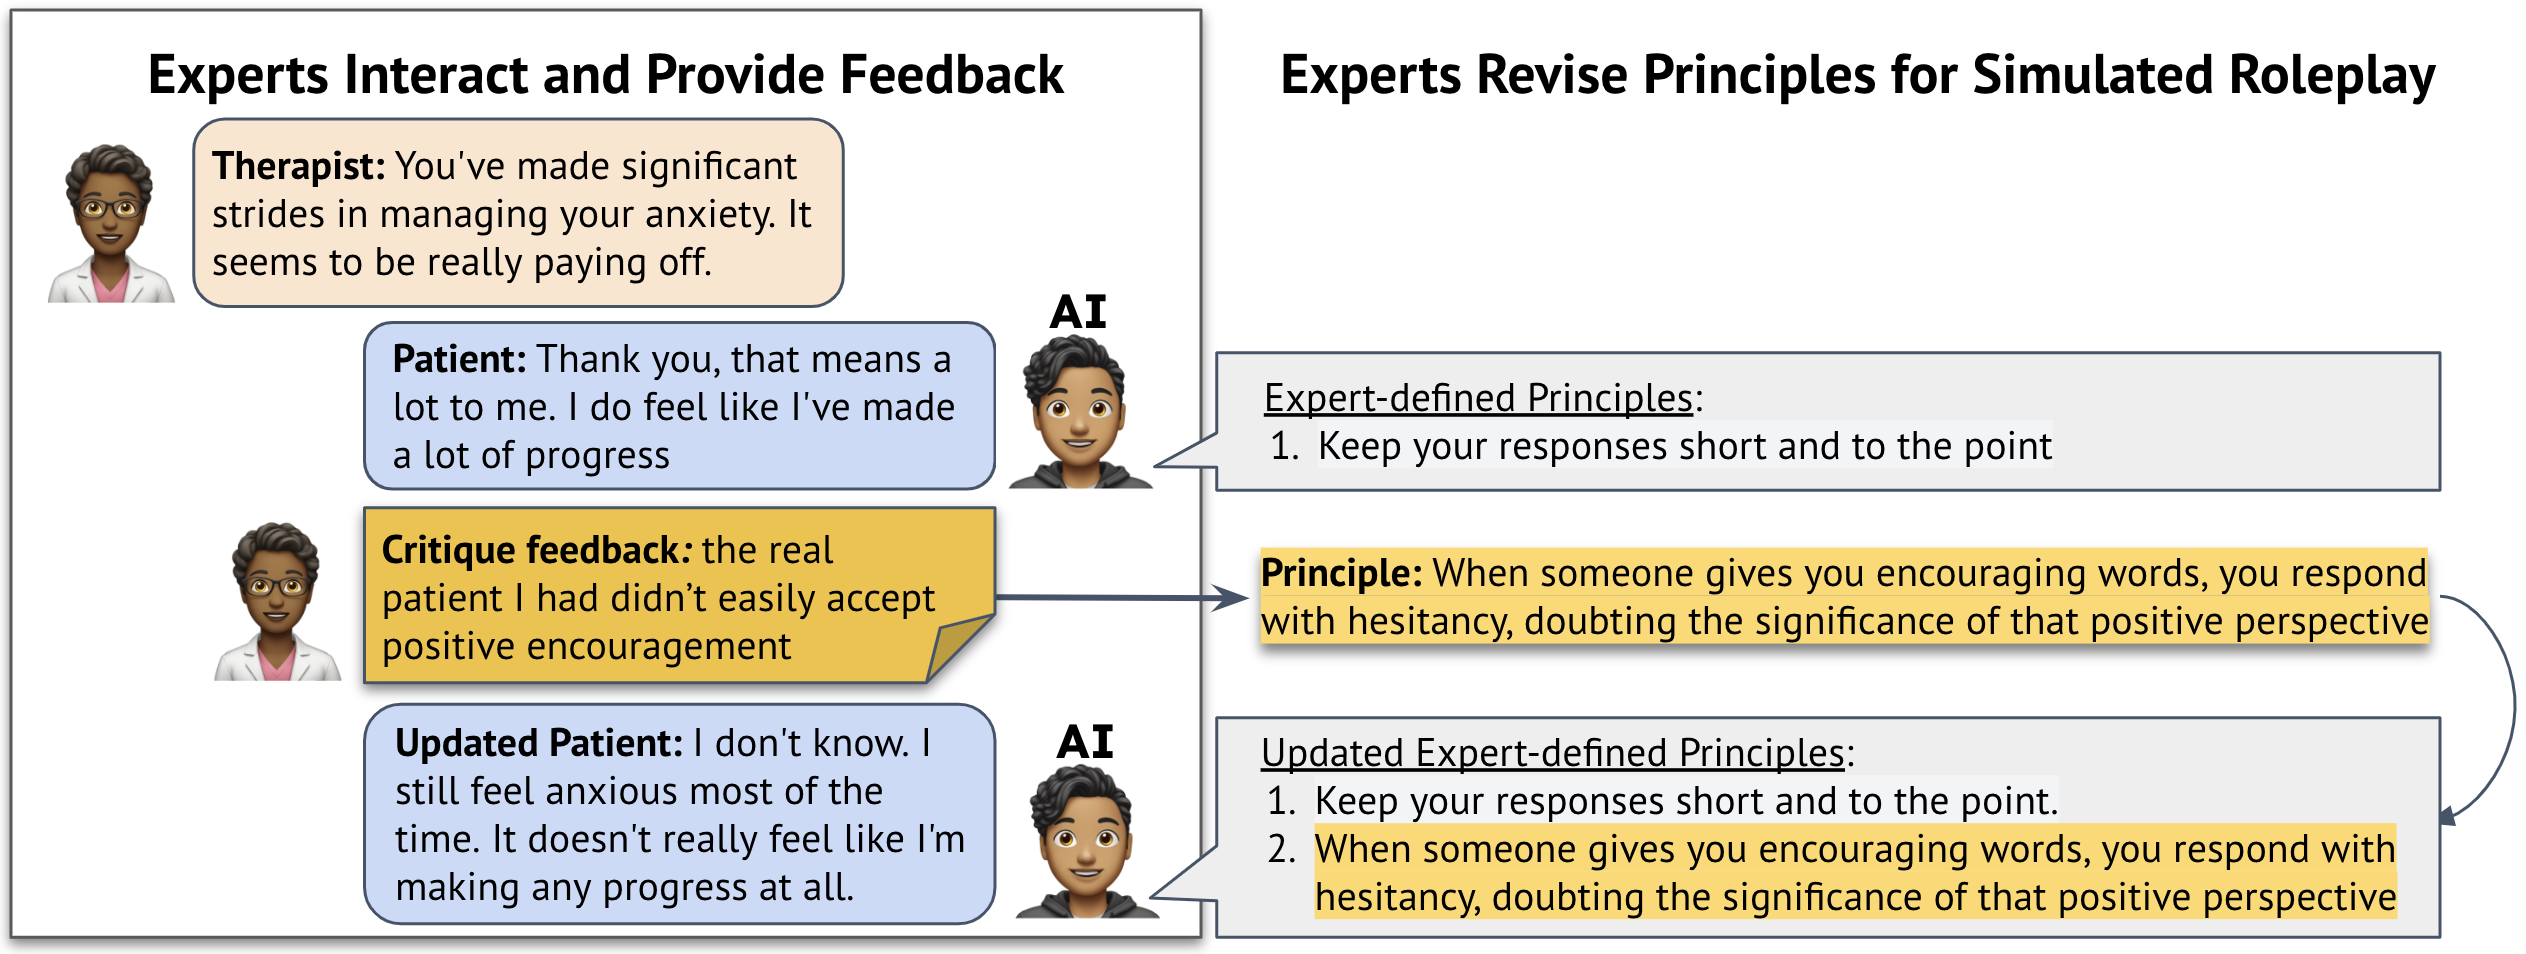
\includegraphics[width=0.98\textwidth]{figures/rpdteaser-clean.png}
    \caption{Roleplay-doh empowers an expert counselor to create a customized AI patient intended for other novice counselors to use as a practice partner. While interacting with the AI patient, the expert counselor can provide qualitative feedback which is converted by an LLM into a principle, or a custom rule governing desired roleplay behavior. The principle is appended to the AI Patient's Constitution }
    \label{fig:rpdteaser}
\end{figure*}
% that governs the patient's roleplay. The AI patient references the latest AI Patient Constitution to generate responses that follow the expert-defined principles.

% \raj{The following paragraph appears as something you would want in related works. Maybe replace this paragraph with "Simulation of AI patient personas is an open challenge in the space... While previous works have tried different prompting approaches, they have failed to resemble typical behaviors of real-patients such as using colloquial language and showing resistance to help. Such AI patients are less useful roleplay partners for novice counselors if they make practice artificial and easy by not faithfully simulating challenges encountered in real-world counseling sessions.}

% Faithful LLM simulations of social scenarios in domains like counseling is an open-challenge. Fine-tuning methods~\cite{demasi-etal-2020-multi} are less viable since mental health data is difficult to obtain due to privacy concerns. While previous works have tested best prompting practices for LLM simulations, they have failed to resemble typical behaviors of real-patients such as using colloquial language and showing resistance to help when first evaluated by mental health experts. Thus, LLM-prompted simulations of AI patients need \textit{experts-in-the-loop} to guide their evaluation and refinement~\cite{chen2023llmempowered, stapleton2023seeing}. However, it remains an open question of how to obtain feedback from domain-experts in a manner that is less tedious and expensive than collecting verbal feedback for prompt iteration, or ranked responses for preference-tuning~\cite{rafailov2024direct}. 

% Recent studies have explored the use of LLMs to create AI patients 
% ~\citep{tanana2019development, demasi-etal-2020-multi, chen2023llmempowered}. While past methods fine-tuned models to clone multiple persona~\cite{demasi-etal-2020-multi}, this approach cannot create custom personas without a dataset and therefore is limited when data is difficult to obtain due to privacy concerns. More recent techniques involve directly prompting LLMs to emulate a patient persona~\cite{chiu2024computational, tu2024conversational}. 
% However, direct persona prompting, when evaluated by experienced counselors, failed to resemble typical behaviors of real-patients such as using colloquial language and showing resistance to help~\cite{chen2023llmempowered}. 
% Such AI patients are less useful roleplay partners for novice counselors if they make practice artificially easy by not faithfully simulating challenges encountered in real-world counseling sessions. 

% \raj{In the next line, can we just say that Realistic simulation of AI patient needs a "Domain expert in the loop"? I am not sure about the word "enhance" here}

% Thus, incorporating domain-expert feedback is essential for enhancing the realism of LLM-simulations. Domain experts, such as psychiatrists~\cite{chen2023llmempowered} or patients with lived experiences~\cite{stapleton2023seeing}, can provide verbal feedback to researchers that guides prompt development. Popular methods for aligning models with human feedback involve collecting preference feedback for model re-training~\cite{christiano2017deep, rafailov2024direct} but can be tedious and time-consuming especially for domain-experts.
% In settings like mental health where expert feedback is costly, there is a need for more efficient methods that allow expert counselors to provide qualitative feedback to refine AI simulations to better mimic realistic patient behavior. 

% In response, we propose RolePlaydoh .... . We perform pilot tests to validate its performance in the domain of mental health.... Our work both points out limitations in existing simulation systems when used in highly specialized domains, and proposes an effective and performant solution (backed by in-depth expert validation studies).... We believe RolePlaydoh can be used to build effective simulation systems for a wide variety of domains, with appropriate expert feedback.

% \raj{the following paragraph can be shortened: describe how we wish to enable human AI collaboration for the realistic simulation by creating an interactive tool that puts therapists in the drivers seat. This is done with the help of constitutions and incremental AI principle building.}
% In response, we aim to enable human-LLM collaboration for realistic simulation by developing an interactive tool, called Roleplay-doh, that empowers therapists to create and refine AI patients on their own.
% \ryan{In previous paragraph, need some help transitioning and building up the idea of roleplay simulations, and distinguishing them from chat/task-oriented assistants}
To address this limitation, we aim to enable human-LLM collaboration for realistic simulation by developing a novel interactive tool, called Roleplay-doh, that empowers domain experts to \textit{directly} guide the creation of simulations by providing \textit{qualitative feedback without any explicit prompting}. 
%We perform pilot tests to validate RolePlay-doh's effectiveness for the task of creating AI patients as roleplay partners for counselors.
% patient that could eventually be used by a novice counselor for realistic practice. 
% \raj{For clarification, do you study how to design or do you design a collaboration pipeline? Which one is the contribution?}
% Explain design goals for roleplay? Then we can say why a recent paradigm would be applicable?
% Since counselors may not know how to prompt LLMs to simulate desired personas and behaviors~\cite{whyjohnnycantprompt}, 
% the pipeline should give them the ease and flexibility of giving feedback in their own words while still effectively steering the simulation. Second, since counseling experts may have multiple behaviors to customize, its useful to be able to rapidly test and iterate on different aspects of their simulation, which rules out methods requiring model re-training. Towards these design goals,
% \raj{Recency in the next line is not a research goal and may not be a good adjective}
Our initial tool design adopts an intuitive and effective paradigm for user-driven chatbot assistant design~\cite{petridis2023constitutionmaker}: experts customize a set of \textit{principles}, or rules written in natural language that govern its behavior \cite{bai2022constitutional}--by (1) interactively critiquing responses in natural language that then (2) gets transformed by an LLM into well-formulated principles describing how the LLM simulation should act from now on \textit{for example, "Respond to encouraging words with hesitation, doubting their significance"} (Fig~\ref{fig:rpdteaser}). The principles are then used along with a persona description to generate roleplay responses. 
% customize LLM chatbots by providing qualitative feedback that gets converted into \textit{a principle} or natural language rule that is added to a \textit{constitution} governing the chatbot's behavior~\cite{bai2022constitutional}. 
% \raj{Why say instantiate here?}
% We instantiate our human-LLM collaboration pipeline in \textbf{Roleplay-doh}
% , a tool that allows counselor experts to mold the behavior of a customized, LLM-powered AI patient
% (Fig~\ref{fig:rpdteaser}), a system for expert counselors to create an AI patient by describing its scenario and customizing its roleplay behaviors by providing free-form or gold-response feedback while interacting. An LLM module helps to convert expert feedback into a well-specified principle that the AI patient should follow when generating future responses, \textit{i.e., "Respond to encouraging words with hesitation, doubting their significance".} 
% Then, the LLM-simulation generates the patient's future responses according to a constitution consisting of these expert-defined principles. 

% \raj{Would be helpful to note the research questions or key results. Can we highlight how roleplaydoh is x\% better than out of the box gpt 4? I feel like at this point, the paper should say we design a principle adhering module and stay tuned for other sections to know more about it.}
% From our process testing Roleplay-doh with expert counselors creating AI patients, we also identified obstacles in LLM-simulations reliably producing high-quality responses after expert customization. 
In our initial tests of the tool with expert-counselors, we found that even with expert refinement via principles, the LLM- simulations had difficulty delivering high-quality responses consistently.
Our analysis of GPT-4 prompted simulation revealed that in 20\% of responses, the simulation had difficulty adhering to multipart principles and misapplying those principles that are only applicable in specific contexts e.g., \textit{only when the therapist provides encouraging words}.
To resolve these issues, we introduce a novel \textbf{principle-adherence pipeline} in the final tool design. The first stage in the pipeline decomposes multipart and contextual principles into a set of yes/no questions that are easier to judge, and the second stage assesses the applicability of each simplified principle to the current scenario before self-refining~\cite{madaan2023selfrefine} the AI patient response as required.
% \ryan{Not exactly accurate, since the first stage also adds principle questions regarding conventions like dialogue coherence and consistency.}
%following the expert-defined principles or conventions like dialogue coherence and consistency.

\if 0
% OLD VERSION WRITTEN BY ANANJAN
Via formative studies with expert counselors,
% Via pilot testing with expert counselors, 
% we uncover that directly prompting GPT-4 to simulate the AI patient's scenario and expert-defined principles results in poor
we uncover that this design results in poor responses in 20\% of cases; an error case analysis showed that the simulation had difficulty adhering to multipart principles and misapplying those principles that are only applicable in specific contexts e.g., \textit{only when the therapist provides encouraging words}.
% , primarily due to errors in adhering to multipart principles and misapplying those that are only applicable in specific contexts e.g., \textit{only when the therapist provides encouraging words}.
% due to errors in adhering to \textit{all} principles, \textit{only in applicable situations}, and \textit{without violating persona or dialogue consistency}.
To resolve these issues, we introduce a novel 
% \textbf{principle-adherence prompting chain
\textbf{principle-adherence pipeline
} in the final tool design. The first step in the pipeline decomposes multipart and contextual principles into a set of yes/no questions that are easier to judge, and the second step assesses the applicability of each simplified principle to the current scenario before self-refining~\cite{madaan2023selfrefine} the AI patient response as required.
\fi

% within the dialogue-simulation pipeline which \textit{critiques} a candidate response for principle-adherence and \textit{revises} the response according to the critique. While similar to recent methods for self-refining LLM outputs~\cite{madaan2023selfrefine}, our principle-adherence pipeline is specifically designed to (1) decompose multipart and contextual principles into a set of yes/no questions that are easier to judge and (2) assess the applicability of principles to the dialogue context (Fig~\ref{fig:principle-adherence-pipeline}). 

% \raj{First time in the paper I feel the word rapidly has popped up, there is no notion of time in as a positive of roleplaydoh before this. I also feel like I know what a scenario only method is but making it explicit will be really helpful.}
% Our evaluation of Roleplay-doh studies the effectiveness of its human-LLM collaboration pipeline in using expert feedback to create and refine AI patients that are more authentic and ready for training. 
% We perform an in-depth evaluation of Roleplay-doh to study the effectiveness of its human-LLM collaboration pipeline in using expert feedback to create and refine AI patients that are more authentic and ready for training. 
We conducted a detailed evaluation of Roleplay-doh to assess its human-LLM collaboration pipeline, focusing on how expert feedback helps develop more authentic AI patients for training. 
% We conduct a within-subjects study with 25 expert counselor, in which they created AI patients by describing a challenging scenario with a real-patient versus using Roleplay-doh to define principles to refine the simulation. 
In a within-subjects study involving 25 expert counselors, participants created AI patients either by describing real-patient scenarios or by using Roleplay-doh to refine simulation principles. 
% We find that Roleplay-doh empowers counselors to create AI patients that are more authentic, greater resemble real-patient cases, and perceived as more ready to be used and recommended as practice partners.  
% Our findings indicate that Roleplay-doh enables counselors to generate AI patients that are not only more authentic and closely mirror real cases, but are also better prepared for use and recommended as practice partners.
The results show that Roleplay-doh enables counselors to produce AI patients that are more authentic, closely resemble real cases, and are better prepared for training use, as judged by creators and third-party counselors.
% --as judged by counselor self-report and 5 counselor's acting as a third-party annotator. 
Further, our principle-adherence pipeline achieves the highest principle following (W: 35\%; L: 5\%) and dialogue consistency (W: 35\%; L: 10\%) compared to all ablations, where preferences are made against a baseline that does not self-refine its output. 
% method performs better than [$\texttt{No Critique}$] on \textbf{M1} (W: 35\%; L 10\%) and on \textbf{M3} (W: 35\%; L 5\%), where it has the highest win/loss rates compared to all ablations.
This work highlights the limitations of existing LLM simulation systems in specialized, data-scarce domains like mental health counseling, and designs and validates a tool that enables expert counselors to directly customize LLM simulations of AI patients.
%Our work thus points out limitations in existing LLM simulation systems when used in the highly specialized domain of mental health counseling, and proposes an effective and performant tool as a solution that is validated by in-depth user studies involving domain experts.
Since Roleplay-doh does not contain any components specifically tailored for the domain of mental health, we hypothesize that the tool can be used to build realistic LLM simulations for a wide variety of domains, with appropriate expert feedback.
% Though we focus on creating AI patients for counseling training, the insights from Roleplay-doh's human-LLM collaboration pipeline and domain-expert evaluation can be applicable to other areas where the LLMs-simulations can benefit from customization through expert feedback. 
%Through this human-LLM collaboration pipeline, experts in various domains are empowered to create custom LLM simulations via the incorporation of qualitative feedback.

 \vspace{-0.05in}
\section{Related Work}\vspace{-0.05in}
\paragraph{Utility of Simulated Partners}
Simulated partners are used to give social skill learners the needed practice opportunities that textbook knowledge cannot provide. % Trained partners, however, may not always be available to practice, or may not be equipped to simulate a diversity of scenarios. 
Past education software develops digital patient simulations to make simulated partners more accessible~\cite{othlinghaus2020seriousroleplaying} but their tailored dialogue trees limit the contexts for practice. LLMs can overcome this issue by being flexibly configured to convincingly simulate a diverse set of personas~\cite{park2022social} and characters~\cite{park2023generative} and generate responses in a range of contexts. Researchers have thus explored their application for simulation training for teaching~\cite{markel_opferman_landay_piech_2023}, conflict resolution~\cite{rehearsal}, and counseling~\cite{demasi-etal-2020-multi,tanana2019development}. 
Previous work has proposed methods to simulate diverse personas and scenarios, but to make practice more useful and transferable~\cite{alinier2022simulation}, they must ensure simulations are faithful to what is encountered in real-world social situations.

\paragraph{Aligning Simulation with Domain Experts}
Feedback from domain experts is crucial to evaluating and improving the realism of LLM simulations. Recent approaches for aligning to human feedback, like \citet{christiano2017deep} or \citet{rafailov2024direct} depend on large amounts of preference data which requires lots of expert time to collect. A more efficient approach is through alignment to qualitative or natural language feedback \cite{shi2022life}. 
Constitutional AI offers a specific alignment strategy involving natural language principles, which are rules that an LLM should follow~\cite{bai2022constitutional}. 
% A constitution's principles can be used to alter an LLM's prompt, or generate new training data for further fine-tuning as in the original ConstitutionalAI work. 
Since constitutions are an explainable and effective method for customizing model behavior, our tool supports expert counselors in defining constitution principles to customize an AI patient simulation. \citet{petridis2023constitutionmaker} studied the human process for writing principles while interactively critiquing model outputs and discovered that there are many cognitive challenges converting critiques into principles. To address these challenges, they developed a tool that allows the user to provide qualitative feedback on responses which gets converted into constitution principles, which are used to alter the LLM's prompt to steer chatbot responses. Our initial tool design adopts this paradigm to support counseling experts to create and customize AI patients, and the final version extends it with a novel principle-adherence prompting pipeline.
In the mental health area, researchers are involving therapy experts when prompting LLMs for simulation~\cite{chen2023llmempowered, lin2024imbue}. 
% In this way, qualitative feedback is gathered during testing sessions with experts, which informs how a researcher engineers the LLM prompts. 
However, requiring a researcher-in-the-loop to refine prompts hinders the speed of iterative design. Our aim is to enable counseling experts to customize the AI patient's constitution simulations that  to eliminate through our work.
% upon a customized LLM-simulation. 
% In our work, we use a principle elicitation approach to rapidly incorporate a domain experts feedback into customized LLM-simulations.


% \raj{Are there other papers on simulating virtual patients, if yes, you can consider creating a section for that}
\paragraph{Text Generation with LLMs}
Generating dialogue responses that adhere to user-defined principles is a type of constrained text generation problem. Recent work has shown that constrained text generation poses challenges when directly prompting GPT-4~\cite{madaan2023selfrefine, bubeck2023sparks, yao2023collie}. To improve outputs, \citet{yao2023collie} propose a self-refine method and conduct evaluation experiments on a dialogue simulation task where responses are constrained by a general set of criteria such as relevance, consistency, informativeness, and helpfulness. A difference in our setting is responses are constrained by expert-defined principles that are multi-faceted and do not apply in all dialogue contexts. This necessitates new modules that breakdown principles into multiple, consise questions and check theapplicability of principles prior to evaluating them.
% ultimately improving the ability of self-refine to adhere to such criteria. 
\vspace{-0.05in}
\section{Designing for Simulated Roleplay}\vspace{-0.05in}
We take a human-centered design approach to developing a
tool for expert counselors to create and customize an AI patient for eventual use as a simulated training partner. After designing an initial version of our tool, we pilot test it with experienced peer counselors to understand any remaining challenges to effective human-LLM collaboration when creating and customizing an AI patient.

\subsection{Initial Tool Design Rationale} \label{sec:initialtooldesignrationale}
% the tool should give them the ease and flexibility of giving feedback in their own words while still effectively updating the Constitution to steer the simulation. Second, since counseling experts may have multiple behaviors to customize, its useful to be able to rapidly test and iterate on different aspects of their simulation, which rules out methods requiring model re-training. Towards these design goals, 
% We aimed to make it simple for counselors to create and customize an AI patient that is faithful to how a real patient would respond in a real conversation. 

Our initial version of Roleplay-doh 
% without the principle-adherence prompting pipeline. The initial tool 
adopted several of the design features of ~\citet{petridis2023constitutionmaker}'s tool for customizing task-oriented chatbots through interactive feedback. 

\textbf{Principle Elicitation:} Counselors can manually write or edit the AI patient's constitution. However, since users often struggle to formulate their thoughts into principles, our tool helps the counselor transform their feedback into specific principles to make principle writing easier. As counselors interact with an AI patient, for each generated response, they have the option to leave feedback in the form of a "kudos" explaining behavior they want to reinforce, a "critique" explaining any undesirable behavior, or a "rewrite" that demonstrates a more desirable response. Then an LLM is prompted (\S\ref{sec:principle-elicitation-prompts}) to translate qualitative feedback into concrete principles that specify what should happen and when, and that generalize beyond the specifics of the dialogue context in which they are generated (Fig~\ref{fig:rpdteaser}).
% , e.g. \textit{when first asked how you are doing, respond with a general description of your emotions and refrain from sharing your entire background story}. 
% As prior work does not reveal the exact prompts for principle elicitation, we develop our own prompts and include them in Appendix \ref{sec:principle-elicitation-prompts}. 
Early testing revealed that GPT-3.5 was sufficient at translating kudos and critique feedback into principles, while prompting GPT-4 to explain differences in initial and rewrite responses helped with inferring a principle.  

\textbf{Testing Principles:} Likewise, to enable easier testing of principles, our tool supports rewinding the last response of the conversation, and generating a new response based on the updated AI Patient constitution. 
% However, our design differs from ConstitutionMaker that we are supporting domain-experts such as experienced counselors to create AI patients that exhibit behaviors that resemble real patients rather than general chatbots.
One feature that we change is generating a single dialogue response, rather than multiple responses, at a time. We reasoned that counselors can identify ways in which a response does not resemble a real-patient's without needing to see multiple, and that generating a response at a time would make the testing process more manageable and similar to having a normal dialogue. 

\textbf{Simulating AI Patient:} We prompt the LLM to follow the most recent set of constitution principles as in~\citet{petridis2023constitutionmaker} rather fine-tuning the LLM weights as in~\citet{bai2022constitutional}'s constitutional AI framework. Since the tool supports defining and testing principles in an iterative fashion, prompting can make steering model behavior quicker and less expensive. 
% Although we did not explore fine-tuning in this work, fine-tuning open-source models using the final AI patient constitution could be a promising line of future work to achieve cheaper inference costs for a production system.
Our prompt (Appendix~\ref{sec:llmprompts-vanilla}) instructs GPT-4 to simulate a patient's next response in a dialogue as opposed to asking the LLM to roleplay as the patient using a system prompt~\cite{zhou2024real}, as early testing revealed that this can mitigate role consistency issues in which the LLM responds as an AI assistant rather than as a patient. 

\if 0
% \paragraph{D1: \textit{Support an active feedback loop for shaping authentic roleplay in AI patients.}} \raj{would be better to say simulate instead of shape; in the following statement make users and counselors consistent}
% Counselors start by writing a description of a patient scenario, or users can equivalently refer to or select from a list of example scenarios. Then, they can begin chatting with an LLM-powered AI patient whose responses are conditioned on the patient's description and conversation history. To support rapid prototyping of the AI patient's behaviors, the tool adopts a recent paradigm for user-driven chatbot design~\cite{petridis2023constitutionmaker}, in which users can provide qualitative feedback on the AI patient chatbot's response which gets converted by an LLM call into a constitution made of {\em principles} that govern desired chatbot behavior (Fig~\ref{fig:rpdteaser}). \raj{Cna we say "...feedback on the AI patient's response to build a constitution". Why specify LLM call here?}

% \paragraph{D2: \textit{Consistent and Customizable Simulation of Patient Scenario.}} \raj{The following statement is not very clear:} To simulate an AI patient's response, we prompt the LLM as a dialogue simulator as opposed to a system prompt asking the LLM to roleplay as the patient~\cite{zhou2024real}, as we found this can mitigate issues where the LLM produces responses as a chat assistant, rather than as a patient. To support rapid customization of the simulation, we prompt the LLM to follow the most recent set of constitution principles as in~\citet{petridis2023constitutionmaker}, rather than fine-tuning the LLM weights as in~\citet{bai2022constitutional}'s constitutional AI framework. We provide the prompt we used in Appendix~\ref{sec:llmprompts-vanilla}.
\fi

\subsection{Pilot Testing} \label{sec:formative-tests}

% \raj{Would it make sense to say this is a pilot study, and we learn the following two things from it? Potentially cut down on some of the text here, it may be too verbose and can be brought down to half column.}
We pilot tested the tool with 5 counselors who had experience giving support to real patients on an online peer support platform; refer to Appendix \ref{sec:participant-background} and \ref{sec:appendix_formative} for participant backgrounds and the pilot procedure. 
% During a 90-minute session, expert counselors created and customized 2 AI patients on average, as time allowed. 
Additionally, four of the co-authors each conversed with four AI patients created and assessed how well the simulation adhered to the expert-defined principles; refer to Appendix~\ref{appendix-sec:principle-adherence-testing} for details on the procedure and qualifications of the co-authors. Overall, the pilot tests and principle-adherence analysis helped uncover two obstacles to effective simulated roleplay. 

\paragraph{O1: \textit{Defining "realistic" patient behavior is ambiguous}} \label{sec:pilot-o1} 
Counselors felt the tool was easy to use and effective at guiding the AI patient's behavior, as indicated by moderate to high agreement scores on a tool usage questionnaire as shown in Table~\ref{tab:tooluse-formative} in Appendix~\ref{sec:appendix_formative}. % Counselors  noted that they liked that there were multiple ways to provide feedback, and the system could help them formulate them into principles. 
However, the task of creating a 'realistic' AI patient for an imagined scenario was confusing, as counselors have interacted with many types of patients who respond in various, yet equally realistic ways. 
% Determining what constitutes a typical response was difficult. 
This insight helped us re-frame the task in later sessions as recreating a challenging scenario from one's past, which removed the ambiguity of what behaviors are realistic by having them refer to a specific case from memory. 


\paragraph{O2: \textit{20\% of responses produced by GPT-4 don't satisfy expert principles or dialogue conventions.}} \label{sec:pilot-o2}
Specifically, 20\% (55/276) of cases were rated as moderately (3), slightly (2), or not at all satisfying (1) at following all principles and being appropriate to the dialogue context. Further analysis of these cases helped to uncover three sources of error.
% \ryan{TODO: In the appendix, we could show a table of the ratings, broken down by AI patients. Each AI patient was complex, but the very complex AI patient would likely break lots of principles!}
% or \textit{"Sometimes, you ask for advice on how to overcome your concerns such as saing "what should I do"}. 
 \textit{\textbf{Not satisfying multiple principles at once:}} Generated responses could struggle to follow all the principles when there was a large number of principles, or when the provided principles were a complex composition of simpler principles. 
 \textit{\textbf{Awkwardness for Dialogue Context:}} Some responses were also identified as awkward or unnatural given conventions in the dialogue context,  despite not violating the defined principles. For example, in the middle of a conversation, saying
\textit{"Hi, A. Yes that's exactly what I mean. There's a voice that is always critical of myself"} is unnatural because of the use of 'Hi'.
\textit{\textbf{Misapplying Situational Principles:}} While generating a response, the model sometimes incorrectly applied principles, such as \textit{Respond with hesitancy when someone gives you encouraging words}, even when the conditions for their use—receiving encouraging words—were not met.
% We discovered that the model sometimes generated responses based on principles that are only applicable under specific conditions. For instance, consider the principle: \textit{Respond with hesitancy when someone gives you encouraging words.} The model inappropriately applied this rule in situations where the required conditions—receiving encouraging words—were not present. 


\begin{figure*}[t]
    \centering
    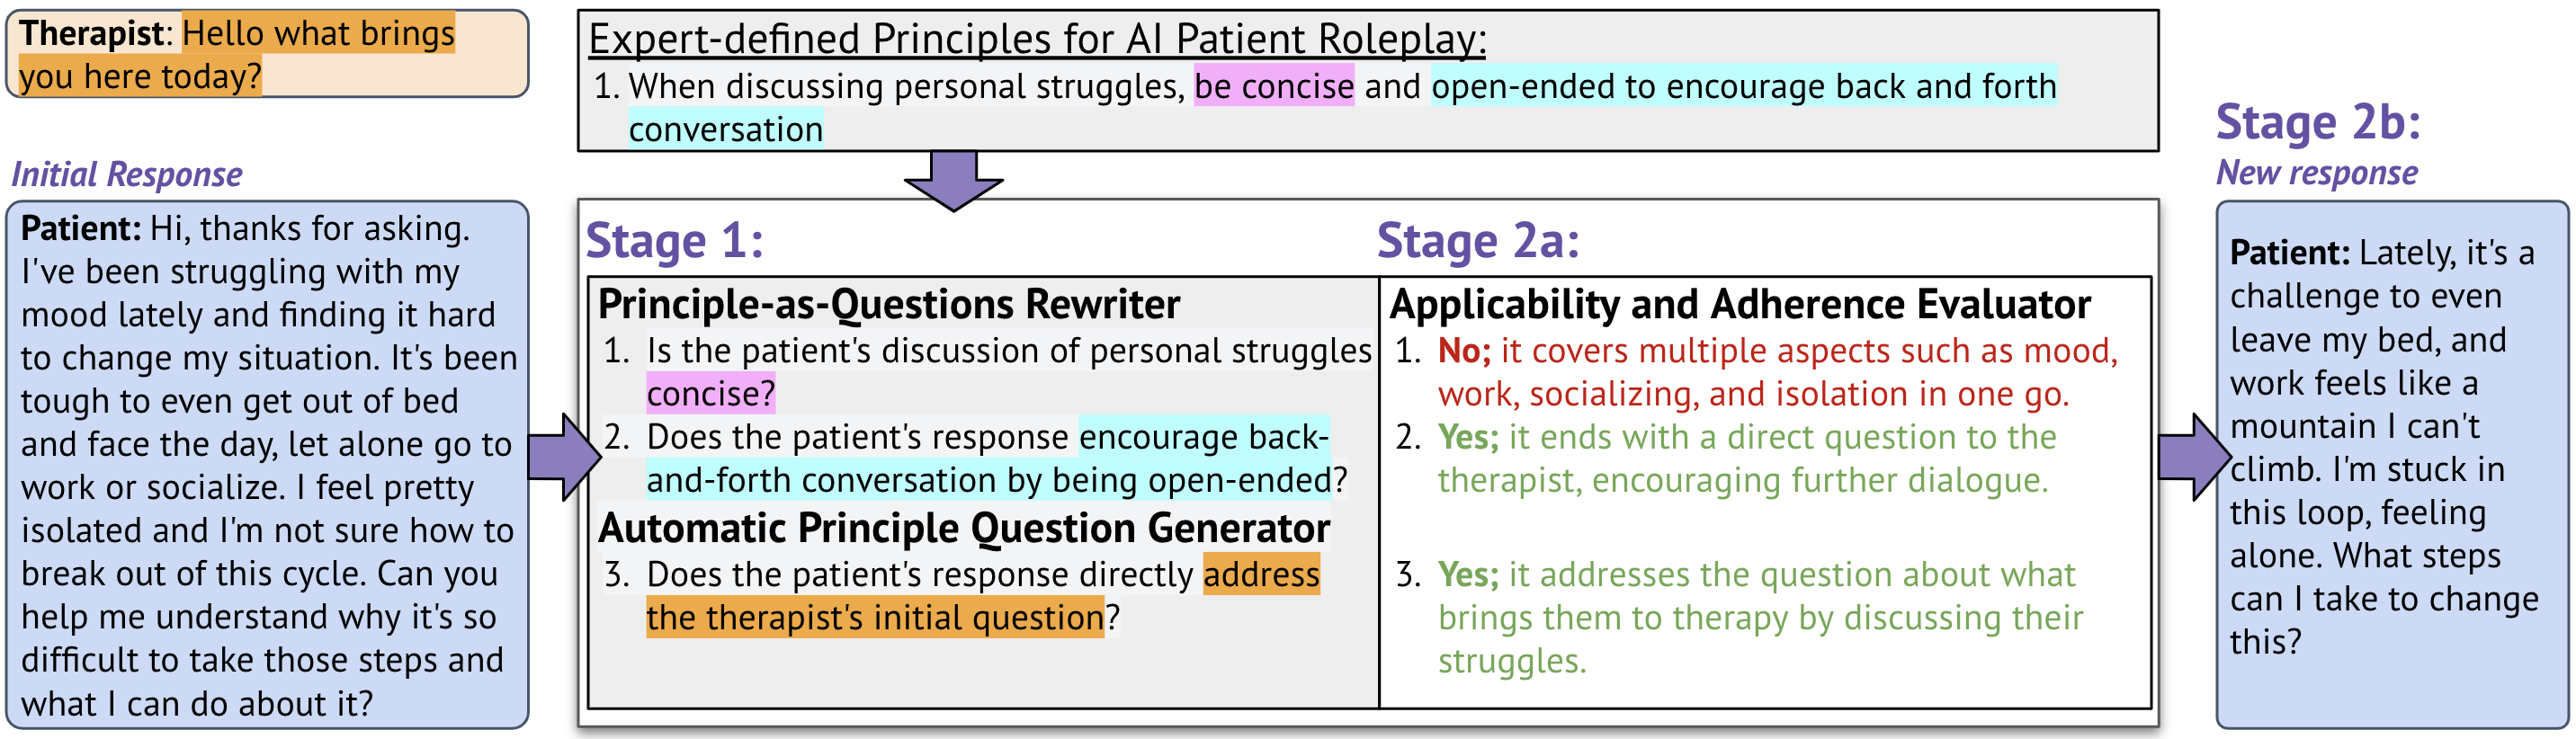
\includegraphics[width=\textwidth]{figures/principle-adherence-stages-colorpop.png}
    \caption{\small{Principle-adherence prompting pipeline for mitigating errors in satisfying expert principles and dialogue conventions. In Stage 1, expert-defined principles are rewritten into several \texttt{Yes/No} questions; and the LLM generates additional principle questions that are relevant to ensure adherence to dialogue conventions such as coherence and consistency. In Stage 2, the LLM (a) evaluates whether the questions are applicable to the context and the answers to the principle-adherence questions; and (b) refines the response to ideally receive \texttt{Yes} on all question.}
    \label{fig:principle-adherence-pipeline}}
\end{figure*}
\vspace{-0.05in}
\section{Roleplay-doh} \vspace{-0.05in}
 \label{sec:roleplaydoh-final-tool}
Roleplay-doh helps counseling experts create customized AI patients based on scenarios from their past experiences. Roleplay-doh uses LLMs in two ways: \emph{Principle Elicitation} and \emph{Response Generation with Principle-Adherence}, which we describe in more detail below: 
% once a counselor gives qualitative feedback on a response, their feedback gets converted into a well-written principle; (2) : as counselors continue chatting, the AI patient uses a principle-adherence pipeline to simulate responses that better adhere to the defined principles. We now describe the methods for performing these tasks.

\paragraph{Principle Elicitation} % 
Roleplay-doh enables counselors to customize an AI patient to resemble a real-patient case by eliciting their qualitative feedback and transforming it into constitution principles that dictate behavior. We provide some examples of principles defined by expert counselors in Table \ref{tab:principle_table}. Since our initial tool design includes the principle elicitation features, we refer the reader to \S\ref{sec:initialtooldesignrationale} for details.

\paragraph{Generation with Principle-Adherence}
We prompt GPT-4 conditioned on patient description, list of principles and conversation history to generate an initial patient response at each conversation turn. Since initial patient responses can fail in 20\% of cases to satisfy expert principles or dialogue conventions, we propose a principle-adherence pipeline that prompts the LLM to generate principle-adherence questions (Stage 1) and employs these questions to assess and refine the initial patient response (Stage 2). 
Our principle-adherence pipeline features three modules to mitigate the identified issues in \S\ref{sec:pilot-o2}. 
% a \textbf{question rewrite} module breaks down the principles into easier-to-evaluate questions, an \textbf{automatic principle generator} identifies additional principles that are relevant for a specific dialogue context, and a \textbf{context-relevant evaluator} ensures only principles that apply to the dialogue context are assessed. Further details on the pipeline's prompt designs can be found in Appendix~\ref{sec:llmprompts}.

\textbf{\textit{Principle-as-Questions Rewriter:}} This module transforms each expert-defined principle into a set of concise yes/no questions that are easier to evaluate for principle-following. Multifacted principles (e.g. “\emph{You should respond in short sentences and avoid using terms like ‘anxious’}”), are divided into separate questions (e.g. “\emph{Does the patient’s response employ short sentences?}” and “\emph{Is the patient’s language devoid of terms like ‘anxious’?}”). % Moreover, this module instructs the LLM to phrase questions to elicit a “Yes” response for proper adherence. For example, the principle “Avoid using metaphors.” is transformed to “Does the response avoid metaphors?” This provides uniformity in assessment of principles with logical negations.

\textbf{\textit{Automatic Principle Generator:}}
This module adds additional principle questions that capture criteria essential for ensuring that the LLM simulation's responses follow general dialogue conventions, such as coherence and consistency. This helps correct cases where there is awkwardness in the generated responses not captured by the defined principles. The LLM is instructed not to make assumptions about the patient or therapist's personality when generating criteria: for example, "\emph{The patient should be appreciative of the therapist's help"} is not an appropriate criterion.

\textbf{\textit{Applicability and Adherence Evaluator:}} % \raj{Can you say this is an NLI task for measuring adherence to the criteria? I feel context-relevance is hard to follow.}
This module determines if each principle is applicable in a given situation, returning \texttt{N/A} if the question is not relevant to answer; otherwise, it evaluates the response using the questions, returning \texttt{Yes} if the response adheres to the principle questions; and \texttt{No} otherwise. For an example of situational applicability, the principle \textit{Show willingness to engage in a suggested activity by affirming the proposal} is evaluated only if the therapist suggests an activity. In situations where the therapist is asking something else and no activity is proposed, the module would appropriately return \texttt{N/A} recognizing that the principle does not apply.

Our pipeline first uses the \textbf{principle-as-questions rewriter} and \textbf{automatic principle generator} modules to generate a set of criteria for evaluating the initial generated response. Then, the response is evaluated using the question by the \textbf{applicability and adherence evaluator}. If the model returns a "No" response for any of the questions, we then perform a rewrite of the response conditioned on the evaluation results, that ideally passes all questions (Fig~\ref{fig:principle-adherence-pipeline}). We detail the prompts used and the procedure used to develop the prompts (\S\ref{sec:principle-adherence-prompts}) and the results of a performance evaluation against ablations (\S\ref{sec:evalpap}). 
\vspace{-0.05in}
% \raj{In this section, was there a part that tries to ablate on the quality of each module? Like the quality of the automatic principle re-writer/ generator?}
\section{User Study using Roleplay-doh}\vspace{-0.05in}
% Transition, and Goals of Study
% To evaluate how Roleplay-doh can aid counseling experts in creating AI patients, we conducted a within-subjects study with 25 participants. We compared two methods for constructing a simulated patient seeking help: (1) a \emph{Scenario-only} dialogue simulation, where the counselor writes a patient scenario description, and (2) a \emph{Scenario+Expert-principles} dialogue simulation, where the counselor uses Roleplay-doh to add interactive principles.
To evaluate how Roleplay-doh can aid counseling experts in creating AI patients, we conducted a within-subjects study with 25 counseling experts, comparing: (1) a \emph{Scenario-only} dialogue simulation, where the counselor writes a patient scenario description, and (2) a \emph{Scenario+Expert-principles} simulation, where the counselor uses Roleplay-doh to define principles. See \S\ref{sec:userflow} for full study setup.

We evaluate the AI patients created by counselors on criteria inspired by prior work evaluating Standardized Patients, who are trained human actors, on their ability to roleplay a case~\cite{himmelbauer2018standardized}. Counselors rated the two AI patients based on 6 dimensions (Table~\ref{tab:measures-roleplay}).
% the \textit{authenticity} and \textit{consistency} in playing the role, their ability to closely \textit{resemble a past case} and mirror its \textit{challenging aspects}, and finally their \textit{role readiness} for usage in peer counselor training. 
We also surveyed each counselor about their experience using the tool for defining principles. 
% Roleplay-doh's features should make it easy and efficient to create expert principles which guide the LLM-simulated patient. 
% As Roleplay-doh's principle elicitation features take inspiration from 
Following \newcite{petridis2023constitutionmaker}, we include four measures for evaluating principle elicitation features (Table~\ref{tab:measures-tooluse}).
% :  which ask about the \textit{ease} and \textit{efficiency in defining principles}, whether participants could write rules to \textit{effectively guide} the AI patients behaviors, and whether the process was \textit{mentally demanding}. 

We recruit 25 counseling experts with real-world experience in mental health support to perform the evaluation, categorized by their primary expertise: 1) those who are pursuing or have completed degrees in counseling or clinical psychology with practicum experience; 2) those who provided online counseling to over 30 clients on the 7 Cups platform; and 3) peer counselors who have provided in-person or virtual support. 

% N = 17
    % \begin{tabular}{|l|c|l|} \hline 
    %       \textbf{Measure}&\textbf{Scenario Only}&\textbf{+ Principles}\\ \hline 
    %       Authenticity&5.00&+0.94 ** \\ \hline 
    %       Stayed in Role&6.18&+0.12\\ \hline 
    %       Resembled Past Case&4.82&+0.94 * \\ \hline 
    %       Mirrored Hard Aspects &4.35&+1.24 * \\ \hline 
    %       Ready as Training Partner&4.94&+1.12 ***  \\ \hline 
    %       Recommend to Novices&5.52&+0.88 ** \\ \hline
    % \end{tabular}

% Colab: https://colab.research.google.com/drive/1xjLde7Ag9sxaOSZm1W3TB6Qmrmzfngtv#scrollTo=Q-03EAvKWOc0
% multiple hypothesis calculation: https://docs.google.com/spreadsheets/d/1e_qhwnNqj4P467n52Yn5EmHt1d_8g4CuFHNH3vQhExE/edit#gid=510140482
\begin{table}[t]
    \centering
    \resizebox{0.485\textwidth}{!}{
    \begin{tabular}{|l|c|l|} \hline 
          \textbf{Measure}&\textbf{Scenario Only}&\textbf{+ Principles}\\ \hline 
          Authenticity&5.24&+0.80 ** \\ \hline 
          Stayed in Role&6.32&+0.08\\ \hline 
          Resembled Past Case&4.8&+0.76 * \\ \hline 
          Mirrored Hard Aspects &4.52&+1.00 * \\ \hline 
          Ready as Training Partner&5.16&+0.64 *  \\ \hline 
          Recommend to Novices&5.76&+0.52 * \\ \hline
    \end{tabular}
    }
    \caption{\small{Creators (N=25) rated their own \textit{Scenario-Only} vs \textit{Scenario+Expert Principles} AI patients along six measures using a 7-point Likert-scale. After refining the AI patient simulation with Expert Principles, creators rate the patient significantly higher on all measures except for \textit{stayed in role}, for which both AI patients score highly. 
    %Results remain significant after using the ~\citet{benjamini1995controlling} method to correct for multiple comparisons ($Q=0.05$). 
    (***:$p<.001$, **:$p<0.01$, *:$p<0.05$., .:$p<0.1$)}}
    \label{tab:creatorstudy-comparison}
\end{table}

% \begin{figure}[t]
%     \centering
%     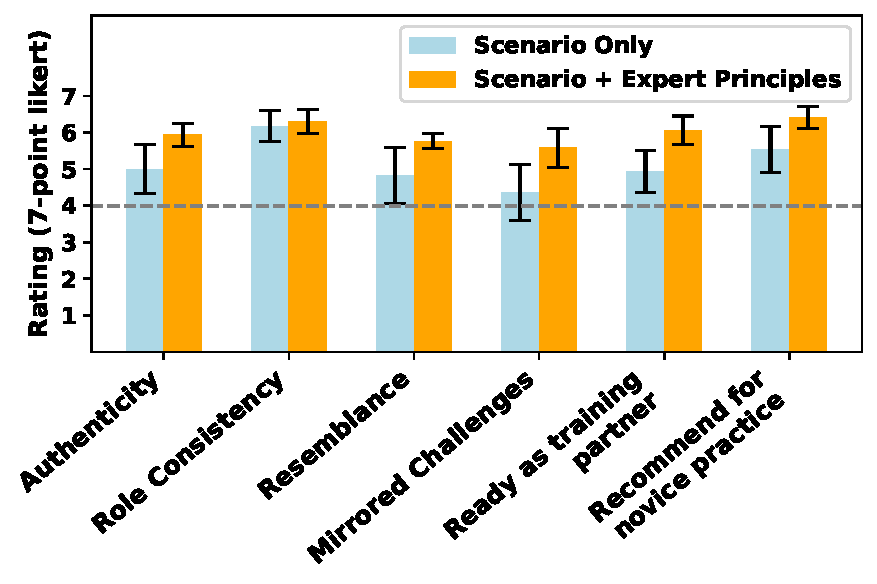
\includegraphics[width=\columnwidth]{figures/creatorstudy-ratings.pdf}
%     \caption{\small{Creator ratings of AI patients. \emph{Scenario+Expert Principles} shows a significantly higher score than \emph{Scenario Only} on authenticity ($\mu_2=5.9$, $\mu_1=5.0$, **, $d=.66$), resemblance to past case ($\mu_2=5.8$, $\mu_1=4.8$, *, $d=.59$), mirroring challenging aspects ($\mu_2=5.6$, $\mu_1=4.4$, *, $d=.76$), readiness as training partner ($\mu_2=6.0$, $\mu_1=4.9$, ***, $d=.93$), and recommendation for novices ($\mu_2=6.4$, $\mu_1=5.5$, **, $d=.66$). No difference was found for role consistency ($\mu_2=6.3$, $\mu_1=6.2$, $d=.13$). Results remain significant after using the ~\citet{benjamini1995controlling} method to correct for multiple comparisons ($Q=0.05$). (***:$p<.001$, **:$p<0.01$, *:$p<0.05$. $d$: Cohen's $d$ calculated by dividing by $\sigma_1$ of control group.}}
%     \label{fig:creatorstudy-comparison}
% \end{figure}


\begin{table}[t]
    \centering
    \resizebox{0.485\textwidth}{!}{
    \begin{tabular}{|l|c|l|} \hline 
          \textbf{Measure}&\textbf{Scenario Only}&\textbf{+ Principles}\\ \hline 
          Authenticity&5.32&+0.31 * \\ \hline 
          Stayed in Role&6.29&+0.09\\ \hline 
          Resembled Typical Cases&4.91&+0.49 ** \\ \hline 
          Challenged the Counselor&2.13&+0.22 \\ \hline 
          Ready as Training Partner&5.05&+0.39 **  \\ \hline 
          Recommend to Novices&5.03&+0.38 * \\ \hline
    \end{tabular}
    }
    \caption{\small{Third-party counselors (N=5) provided 125 total comparisons of the \textit{Scenario-Only} vs \textit{Scenario+Expert Principles} AI patients along six measures using a 7-point Likert-scale. The treatment effect of adding expert principles was estimated using using the following linear mixed-effect model: \lstinline[]!Rating\~Treatment+CreatorID+(1|AnnotatorID)!}. (***:$p<.001$, **:$p<0.01$, *:$p<0.05$., .:$p<0.1$)}
    \label{tab:thirdpartystudy-comparison}
\end{table}
  
\subsection{Creator Perceptions}\label{sec:firstparty}
% Quantitative - Authenticity, Challenge, Readiness
% Table~\ref{tab:creatorstudy-comparison} shows the results of counselors' ratings of the two AI patients they created. 
The AI patients prompted with \textit{Scenario+Expert Principles} were rated significantly higher than \textit{Scenario-Only} on all measures except for role consistency, for which both methods score highly (Table~\ref{tab:creatorstudy-comparison}).
Counselors mentioned the \textit{Scenario-Only} AI patient \textbf{lacked emotional depth in expression}. As one noted, \textit{"patients don't state a feeling such as 'I feel hopeless'. They display their current emotional state in their manner of speech."} \textit{Scenario-only} was also \textbf{too articulate and forthcoming} when describing issues, where encouraging real patients to share is \textit{"as challenging as pulling teeth"}. It was characterized as \textbf{too cooperative}, too willing to accept. Despite counselors writing behavioral traits such as \textit{"not talkative"} and \textit{"reluctant"} in the patient scenario, \textit{Scenario-only} did not exhibit these behaviors.
% \raj{Raj pass ends here}
\begin{table*}
    % \small
    \footnotesize
    % \tiny
\centering
\resizebox{0.98\textwidth}{!}{%
    \begin{tabular}{|p{0.1cm}|p{.1cm}|p{.1cm}|c|p{5cm}|p{8cm}|} \hline 
          \multicolumn{3}{|c|}{\textbf{Stages}}
          &\textbf{\# AI patients} &  \textbf{Theme} &  \textbf{Example Principle}\\ \hline     \cellcolor{gray!60}&\cellcolor{gray!60}&\cellcolor{gray!60}&14 & Keep responses concise and do not share too much. & When discussing personal struggles, be more concise and open-ended to encourage a back-and-forth conversation.\\ \hline 
           \cellcolor{gray!60}&\cellcolor{gray!60}&\cellcolor{gray!60}&7&  Use colloquial and realistic langauge language.&  Incorporate natural speech patterns, improper grammar and punctuation, including the use of slang and less structured sentences, to convey a more authentic and relatable character.\\ \hline 
           \cellcolor{orange!40}&&&14& Show initial mistrust and hesitation with the idea of seeking help.& When expressing feelings of overwhelm and doubt, provide limited information and express skepticism towards the effectiveness of seeking help. \\ \hline 
          \cellcolor{orange!40}&\cellcolor{blue!30}&&19& Show emotions in detail, elaborating with examples as needed.\colorbox{yellow!30}{*} &  When describing personal struggles, provide specific details and symptoms to help the listener understand the situation better.\\ \hline 
          \cellcolor{orange!40}&\cellcolor{blue!30}&&9&  Be less self-aware of emotions, thoughts, and needs. Articulate thoughts in a more disorganized way.&  When expressing reluctance or uncertainty about seeking help or accepting praise, it's important to convey the internal struggle and conflicting emotions, rather than presenting a clear-cut decision or emotion.\\ \hline 
           &\cellcolor{blue!30}&\cellcolor{green!60}&3&Do not seek out solutions, but rather just share thoughts and feelings. \colorbox{yellow!30}{*}&When expressing feelings of being stuck or defeated, focus on sharing emotions rather than seeking a resolution.  \\ \hline
          &&\cellcolor{green!60}&12& Proactively seek out solutions and show reflective insight over time. \colorbox{yellow!30}{*} &  When discussing personal struggles, provide reflective insights into your situation and propose actionable steps for improvement to continue the conversation effectively. \\ \hline 

    \end{tabular}}
    \caption{\small{Themes taken from qualitative analysis of principles and representative examples. We discover several novel (\colorbox{yellow!30}{*}) principles compared to those defined in prior work on AI patients~\cite{chen2023llmempowered, stapleton2023seeing}. Themes are categorized into stages of conversation taken from \cite{DBLP:journals/corr/abs-2106-01144}: \colorbox{orange!40}{exploration}, \colorbox{blue!30}{comforting}, and \colorbox{green!60}{action}; those relating to the overall conversation are categorized as \colorbox{gray!60}{stage-agnostic}.}}
    \label{tab:principle_table}
\end{table*}


\subsection{Creating Principles with Roleplay-doh}
% \diyi{are these new or novel principles we discovered? if so, lets highlight it in Table}
% \textit{\textbf{Analysis of Principles:}} 
% Counselors defined principles with Roleplay-doh to mould a more realistic AI patient. 
Across the 25 \textit{Scenario+ExpertPrinciple} AI patients, 123 total principles were created (min=1, max=10, median=5). Two authors did a qualitative coding of these principles following a thematic analysis approach~\cite{braun2006thematicanalysis} where codes were initially defined and revised during the process.
% Groupings in each stage
Besides \colorbox{gray!60}{stage-agnostic} themes dictating a \textbf{concise} (14 patients) and \textbf{colloquial} (7 patients) speaking style, counselors created principles related to the stages of an emotional support conversation \cite{DBLP:journals/corr/abs-2106-01144}: 1) \colorbox{orange!40}{exploration}: identifying the patient's problems, 2)\colorbox{blue!30}{comforting}: using empathy and understanding to comfort the patient, and 3) \colorbox{green!60}{action}: formulating solutions to the patient's problems. For instance, we find a common theme of instructing the AI patient to \textbf{show initial skepticism with the idea of seeking help} (14 patients), corresponding to the style of interaction in the \colorbox{orange!40}{exploration} stage of conversation. Table \ref{tab:principle_table} provides a full list of principle themes, examples, and corresponding conversation stages. 

While we observe overlaps in the types of principles defined, we also observe some contradictory themes. For example, the call for being \textbf{disorganized and conflicted} (9 patients) contrasts calls to make responses \textbf{concise and direct} (14 patients). In the \colorbox{green!60}{action} stage of conversation, several counselors added principles to make the AI patient \textbf{proactively ask for advice} (12 patients); nonetheless, other counselors added an opposing principle to \textbf{not seek out solutions} but rather just share their thoughts and feelings (3 patients). These opposing principles highlights the need for different principles to describe diverse patient behavior, which challenges the notion of defining AI patients based on a single set of principles. 

\paragraph{Tool User Experience} Counselors found the tool helpful for writing principles that \textbf{effectively guided} the AI patient to recreate their past case ($\mu=6.04$, $\sigma=1.06$). With the tool, most found it \textbf{easy} to convert their thoughts and feedback on the AI patient's behavior into principles ($\mu=6.12$, $\sigma=1.13$). Counselors felt they could \textbf{efficiently} write principles ($\mu=6.3$, $\sigma=1.29$), without requiring much \textbf{mental demand} ($\mu=3.20$, $\sigma=1.70$). 
Many counselors liked how the tools \emph{"organized their thoughts into rules"}, without \emph{"needing to word it perfectly."}
%, [they] just had to say the general idea of what [they] meant."} 
% These ratings and comments are similar to what ~\citet{petridis2023constitutionmaker}'s participants report, which validates the utility of these principle-elicitation features. 
Yet, principle-elicitation did not work perfectly in all cases: 11.4\% of principles required manually editing. 
% Some counselors remained optimistic about the assistance an imperfect LLM could provide: \textit{"having AI there to help write the principles made me think more about what I was writing to make sure it captured everything I wanted it to, and when it didn't, I could just overwrite what it put"} (P5).
Via a worse-case analysis of creators' tool use, we uncover scenarios where Roleplay-doh's human-LLM collaboration pipeline can still be improved (\S\ref{sec:worst-case-tool-experience}). 
% To aid future research aimed at improving the human-LLM collaboration pipeline of customized constitutions, we release a dataset of counselor's fine-grained interactions with Roleplay-doh's principle-elictation features\footnote{https://github.com/SALT-NLP/roleplay-doh}. 
% As the human-centered NLP community has advocated for the sharing of datasets capturing fine-grained interactions in human-LLM co-authoring~\cite{lee2022coauthor}, we release a dataset of counselors defining AI patients constitutions via principle-elicitation so future research can improve the co-authoring of constitutions\footnote{https://github.com/SALT-NLP/roleplay-doh}.



% \begin{figure}[t]
%     \centering
%     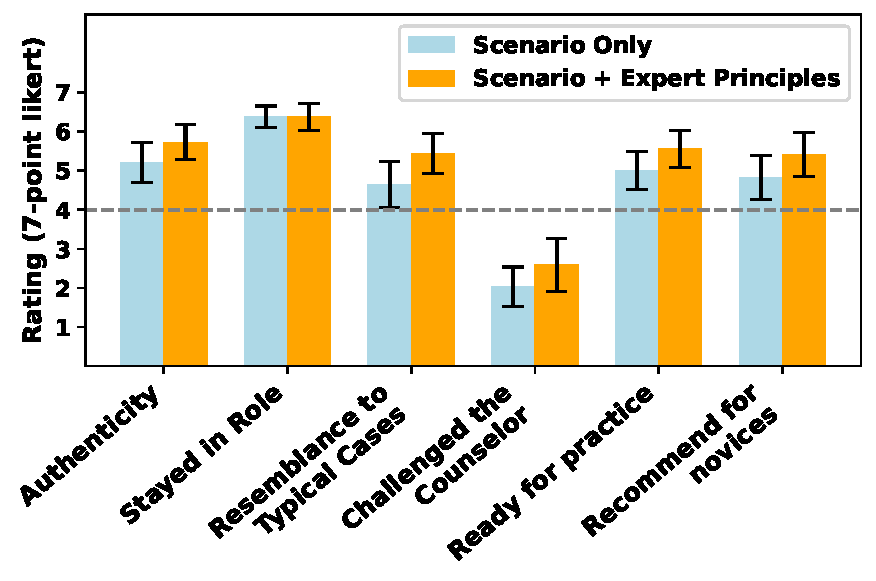
\includegraphics[width=\columnwidth]{figures/thirdparty-ratings.pdf}
%     \caption{\small{Third-party ratings for AI patients. After correcting for multiple hypothesis testing, we report no significant differences on authenticity ($\mu_2=5.7$, $\mu_1=5.2$, p=0.06., $d=.34$), resemblance to typical cases ($\mu_2=5.4$, $\mu_1=4.6$, p=0.01, $d=.45$), challenged the counselor ($\mu_2=2.58$, $\mu_1=2.0$, p=0.049, $d=.37$), readiness as training partner ($\mu_2=5.5$, $\mu_1=5.0$, p=0.03, $d=.39$), and recommendation for novices ($\mu_2=5.4$, $\mu_1=4.8$, p=0.06, $d=.35$). No difference was found for role consistency. }}%  ($\mu_2=6.38$, $\mu_1=6.38$, $d=0$). ($d$: Cohen's $d$ calculated by dividing by $\sigma_1$ of control group.}
%     \label{fig:thirdpartystudy-comparison}
% \end{figure}


% With percentage increase
% \begin{table}[t]
%     \centering
%     \resizebox{0.48\textwidth}{!}{
%     \begin{tabular}{|l|c|l|l|} \hline 
%           \textbf{Measure}&\textbf{Scenario Only}&\textbf{+ Principles}&\textbf{\% increase}\\ \hline 
%           Authenticity&5.28&+0.39 ** &7.4\%\\ \hline 
%           Stayed in Role&6.35&+0.03&0.5\%\\ \hline 
%           Resembled Typical Cases&4.88&+0.64 *** &13.1\%\\ \hline 
%           Challenged the Counselor&2.09&+0.37 . &17.7\%\\ \hline 
%           Ready as Training Partner&5.00&+0.52 **  &10.4\%\\ \hline 
%           Recommend to Novices&5.03&+0.48 * &9.5\%\\ \hline
%     \end{tabular}
%     }
%     \caption{\small{Third-party counselors rated the \textit{Scenario-Only} vs \textit{Scenario+Expert Principles} AI patients along six measures using a 7-point Likert-scale. The treatment effect of adding Expert Principles was estimated using using the following linear mixed-effect model: \lstinline[]!Rating\~Treatment+CreatorID+(1|AnnotatorID)!}. Results are based on 5 annotators providing ratings for both AI patients made by 17 creators.  (***:$p<.001$, **:$p<0.01$, *:$p<0.05$., .:p<0.1)}
%     \label{tab:thirdpartystudy-comparison}
% \end{table}

\subsection{Third-Party Comparison} \label{sec:third-party}
% RQs/Claims/Goal

% The dialogues between counselors and AI patients collected during the creator study allowed us to further investigate our hypothesis about the benefits of roleplay simulations shaped by Expert Principles. 
%While we found in \S\ref{sec:firstparty} that AI patients with expert principles were rated more realistic and useful, 
%One limitation of our creator study in \S\ref{sec:firstparty} is that creators knew which patient had their principles, and thus could be inherently biased to the patient that they spent effort to customize. Thus, we conducted a third-party study in which an external counselor acts as an unbiased judge of the AI patients made by each creator. Judges were shown AI patient transcripts in a randomized order to make judges blind to the condition. We decided to recruit 5 counselors from the creator study whom were similarly qualified to judge the realism of AI patients. Through a power-analysis, we concluded that our statistical test could achieve 80\% power  using 5 third-party judges; see Appendix~\ref{appendix-sec:third-party-power-analysis} for details of the power-analysis.
A limitation of our creator study (\S\ref{sec:firstparty}) is the potential bias from creators who knew which AI patient embodied their principles. To address this, we conducted a third-party study where external counselors served as impartial judges. These judges evaluated AI patient transcripts presented in randomized order to ensure blindness to the condition. We invited five counselors from the creator study to serve as judges, all equally qualified of assessing AI patient realism. A power analysis confirmed that five judges would provide 80\% statistical power (Appendix \S\ref{appendix-sec:third-party-power-analysis}).
% We chose to hide the patient's scenario description; this required judges to rate the AI patient based solely on their responses in the transcript so it could mitigate any bias in knowing what scenario the AI patient was prompted with. % ounselors. 
The third-party counselors rated the same six dimensions as the creator study, with questions reworded for the perspective of external judge (Appendix \S\ref{appendix-sec:thirdparty-detailed-measures}). 
% COMMENTING OUT TO SHORTEN
% Some modifications did not directly translate because a third-party judge does not have the first-hand experience of supporting the real patient upon which the past-case is based. For example, rather than being asked if an AI patient \textit{resembled the behaviors of the past case}, a third-party judges were asked whether the patient \textit{resembled the behaviors that typical patients exhibit.}
% As another example, rather than asking if the patient \textit{mirrored the challenging aspects} of the case, third-party judges were asked whether the patient's behaviors \textit{made it hard for the counselor to give support}.


\begin{figure*}
    \centering
    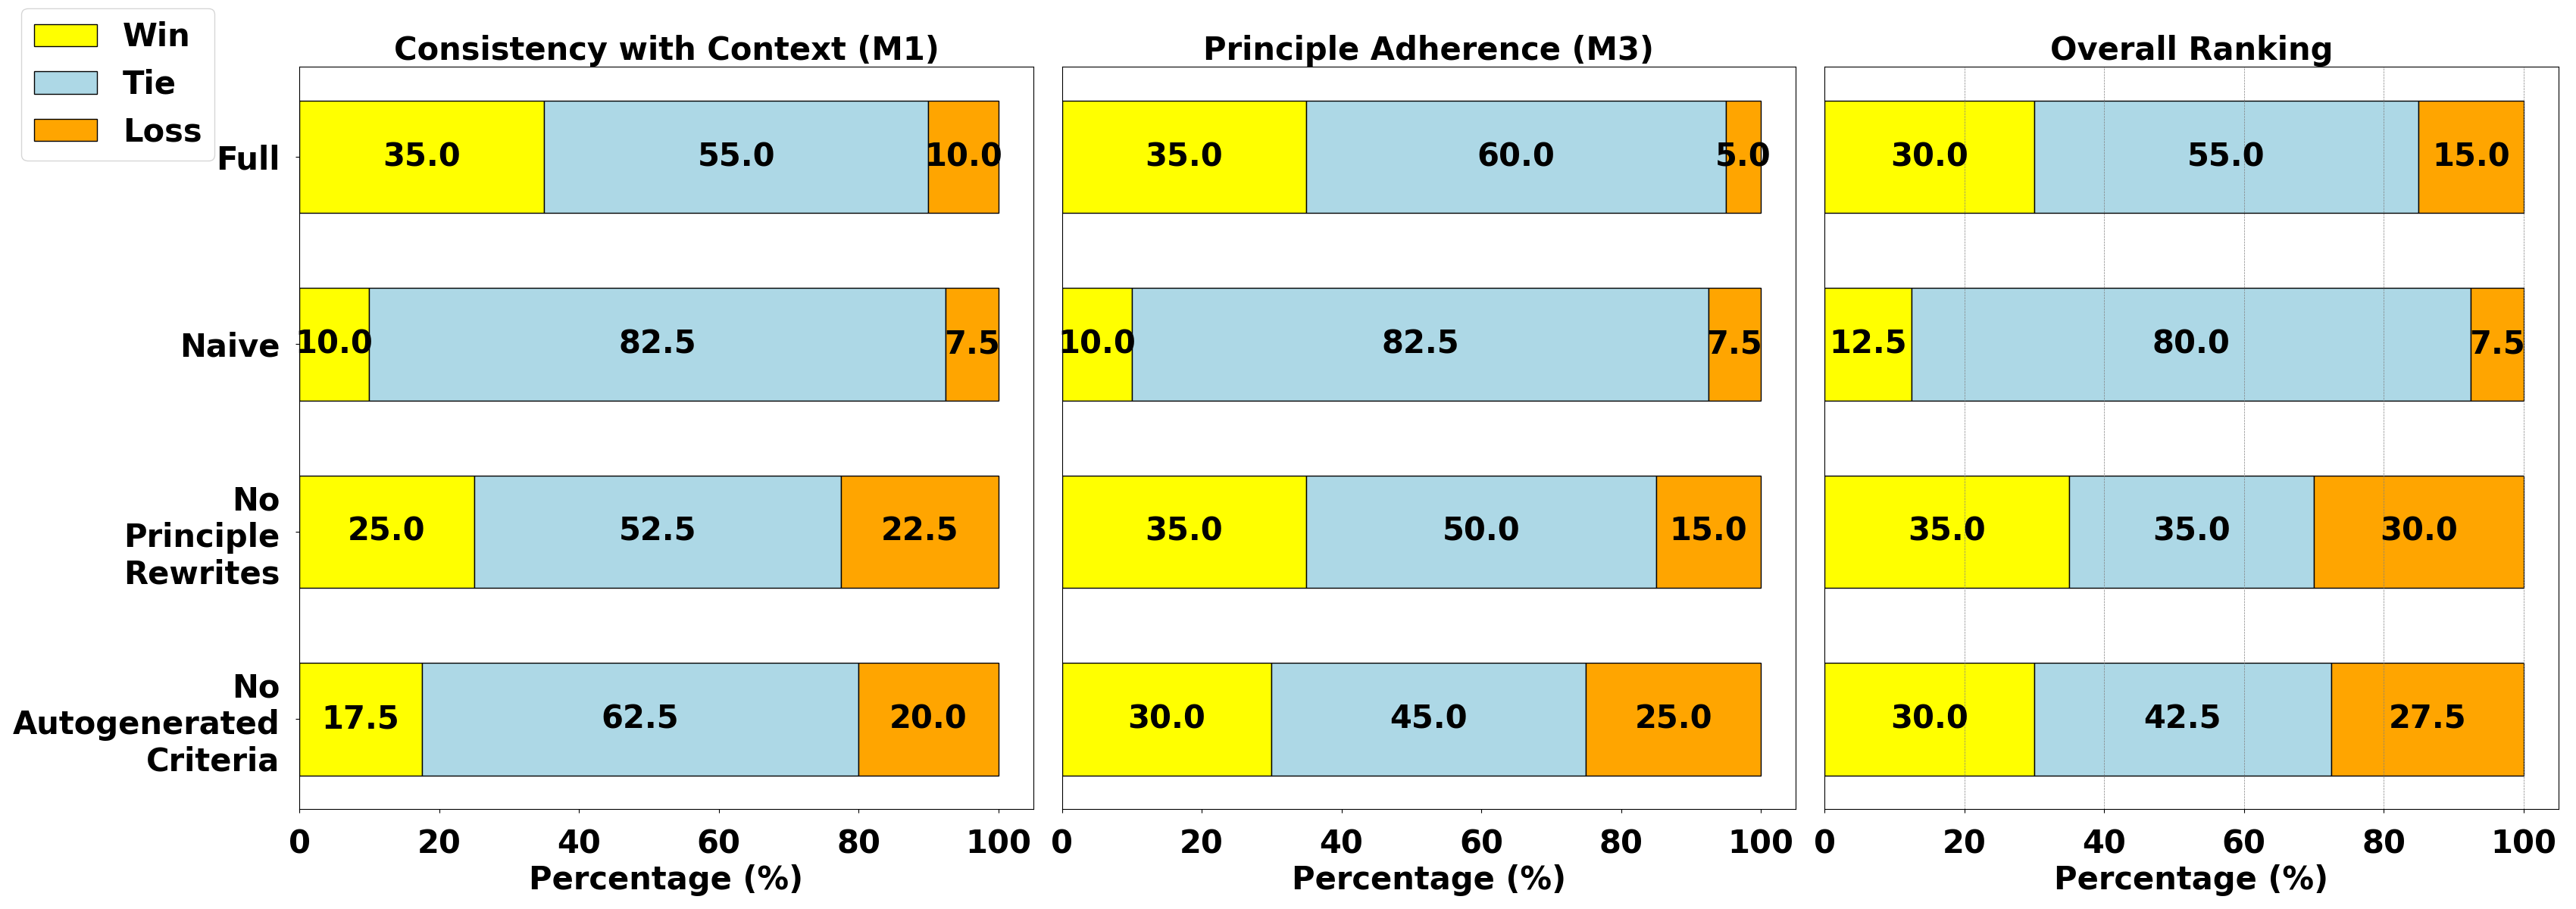
\includegraphics[width=\textwidth]{figures/error_2.png}\vspace{-0.05in}
    \caption{\small{Win/Tie/Loss for the Error Test Cases along \textbf{Consistency with Context (M1)}, \textbf{Principle Adherence (M3)}, and \textbf{Overall}. Pairwise preference evaluation results with [\texttt{No Critique}] as a baseline. Results obtained after majority voting.}}
    \label{fig:wtl-error}
\end{figure*}

% Overall performance
Third-party judges rate AI Patients with expert-defined principles as more authentic, resembling typical cases, ready as a training partner, and likely recommend to novices (Table~\ref{tab:thirdpartystudy-comparison}). 
%The addition of \textit{Expert Principles} increases an AI patient's ratings over the \textit{Scenario-only} counterpart by 0.31 - 0.64 points. 
However, when compared to the creator study results, the increase in ratings is smaller from the perspective of third-party counselors.
% Agreement between third-party counselors is lower but positive (Krippendorf's $\alpha$ is between 0.22 - 0.3 across the six measures), which can explain this smaller effect size.
We explore the reasons for this smaller difference in Appendix~\ref{appendix-sec:thirdparty-qual-analysis}.
We find this disagreement can be attributed to different principles attended to by third-party counselors and the specific principles added by the creator. 
% See Appendix~\ref{appendix-sec:thirdparty-detailed-measures} for detailed analyses.
\vspace{-0.05in}
\section{Evaluation of Principle-Adherence}
\label{sec:evalpap}
\vspace{-0.05in}
% To complement the study of counselors using Roleplay-doh to create AI patients, we 
% This section presents ablation studies of Roleplay-doh's principle-adherence pipeline.
We now evaluate whether the principle-adherence pipeline improves the quality of responses for Roleplay-doh, along with an ablation analysis showcasing the utility of its various components. Specifically, we break down the evaluation of model responses along three metrics: \textbf{M1)} Are they consistent with the patient description and conversation history? \textbf{M2)} Do they exhibit an awkward style of speech? \textbf{M3)} Do they adhere to the provided principles?

We evaluate the performance of our principle-adherence pipeline [$\texttt{Full}$] over (1) GPT-4 response generation without our pipeline [$\texttt{No Critique}$]; (2) an ablation without the \textbf{Principle-as-Questions Rewriter} [$\texttt{No Principle Rewrites}$]; (3) an ablation without the \textbf{Automatic Principle Generator} [$\texttt{No Autogenerated Criteria}$]; and (4) an implementation of the principle-adherence pipeline that does not have any of these modules [$\texttt{Naive}$]. 

To analyze how the pipeline mitigates errors that arise in base GPT-4 generations, 
we select 40 conversation turns from our user study logs that fall into one of the error categories described in \S\ref{sec:formative-tests} as testcases. 
Each testcase contains the scenario, conversation history up to that point, and the expert-defined principles for the AI patient. 
For each test case, responses are generated for all models and then ranked by expert counselors from 1 (best) to 5 (worst) for metrics \textbf{M1} and \textbf{M3}, along with "Yes" or "No" annotations for \textbf{M2}. Finally, experts provide an \textbf{Overall} ranking , along with a brief textual explanation. We allow multiple responses to have the same rank and randomize order of responses to minimize positional bias (details in \S\ref{sec:annotint}).

We treat [$\texttt{No Critique}$] as our baseline and compare all other models to it. 
We report preference results based on majority vote across 3 expert counselor annotations (Fig~\ref{fig:wtl-error}).
% Each testcase is annotated by 3 expert counselors, after which we use majority voting to aggregate results as shown in Fig~\ref{fig:wtl-error}. 
We find our [$\texttt{Full}$] method performs better than [$\texttt{No Critique}$] on \textbf{M1} (W: 35\%; L 10\%) and on \textbf{M3} (W: 35\%; L 5\%), where it has the highest win/loss rates compared to all ablations. On overall rankings, it again has the strongest performance (W: 30\%; L 15\%). We find that the performance of [$\texttt{Full}$] compared to [$\texttt{No Critique}$] is weaker on \textbf{Overall} than $\textbf{M1}$ and $\textbf{M3}$. This is because the annotators often used their own subjective judgements (e.g.,\emph{"although the middle response ranked third on principle following, it feels like the most realistic response in this scenario"}) to perform the overall ranking, resulting in unpredictable and subjective results. We also find that [$\texttt{Naive}$] has a disproportionately high tie rate across metrics, indicating that it rarely produces better responses even for error cases. This highlights the importance of the \textbf{Principle-as-Questions Rewriter} and \textbf{Automatic Principle Generator} for improving responses.  

For \textbf{M2}, 
% we find that for the random testcases, all annotators report no awkward style in any of the responses with perfect agreement. 
after majority voting, annotators report that $2.5\%$ of responses are awkward for the [$\texttt{Full}$] method, as compared to $15\%$ for [$\texttt{No Critique}$], $7.5\%$ for [$\texttt{Naive}$], $7.5\%$ for [$\texttt{No Principle Rewrites}$] and $15\%$ for [$\texttt{No Autogenerated Criteria}$]. Therefore, our principle adherence pipeline substantially reduces the occurrence of awkward style in responses (by a margin of $12.5\%$). The $12.5\%$ gap in percentage of awkward responses between [$\texttt{Full}$] and  [$\texttt{No Autogenerated Criteria}$] also indicates the importance of the \textbf{Automatic Principle Generator} for producing realistic rewrites. We repeat these experiments with 50 randomly picked conversation turns and report results in \S\ref{sec:detres}, along with Krippendorff's $\alpha$ numbers. 

% We find that $\texttt{Full}$ consistently outperforms the other methods considered. It outperforms the $\texttt{No Critique}$ baseline by a maximum of 59 Elo rating points and the $\texttt{Naive}$ self-critique module by a maximum of 50 Elo rating points, highlighting the gains obtained by our tailored approach. $\texttt{Full}$ outperforms $\texttt{No Rewrite}$ by a maximum margin of 40 Elo rating points and $\texttt{No Autogen}$ by a maximum margin of 110 Elo rating points, highlighting the importance of the principle rewrite and automatically generated principle modules \ananjan{These need better names, can be introduced in Section 4}. 

% While investigating the relatively low annotator agreement scores, we find that the self-critique module is especially effective when the original response contains blatant stylistic errors (such as starting every sentence with "Hi") and when the original response contains information inconsistent with conversation history. For similar responses, the annotators often use a subjective notion of which response is more "consistent" with the previous conversation to assign ranking, rather than purely evaluating principle following. This notion is often inconsistent between annotators.

% Therefore, we additionally validate that our self-critique module does not result in a decrease in output quality when the original response from GPT-4 is already of sufficient quality. We randomly pick 20 testcases from the formative study that were not critiqued by the users. Annotators are provided with the original responses and the responses from the principle-adherence pipeline in randomized orders, along with the original set of principles, the description of the persona of the patient, and the conversation history till that point for context, and assign scores on a Likert scale of -1,0,1 to the statement "The first response is substantially better than the second one in the given context". If the response from the self critique module is the second response, we invert the corresponding Likert score before aggregating. Each testcase is scored by 2 annotators.  

% The average Likert score obtained over these testcases is \textbf{0.1} for one annotator and \textbf{-0.1} for the other annotator. \textbf{DISCUSSION OF RESULTS HERE}

% We conclude that our principle-adherence pipelines produces responses that are better at principle-following and are more relevant to the dialogue context.

% \ryan{Note: These are expected findings, this comparison study has not been completed.} \ananjan{emphasis on gains from our method once we have numbers.}



% \subsection{Analysis of Simulated-Dialogues}
% %by Third-Party Human Judges and Automatic Metrics
% The dialogues between counselors and AI patients were collected during the creator study allowed us to further investigate our hypothesis about the benefits of roleplay simulations shaped by Expert Principles. We evaluate the simulated-dialogues with a \textit{Scenario-Only} vs. \textit{Scenario+ExpertPrinciples} AI patient from the perspective of third-party counselors comparing AI patients made by other counselor's, and through automatic content analysis of the dialogues.


\vspace{-0.05in}
\section{Conclusions}\vspace{-0.05in}
This paper introduces Roleplay-doh, a tool that empowers domain experts to create 
LLM simulations through the automatic conversion of expert feedback into natural language principles, and validates the tool for the task of creating  AI patients that serve as roleplay partners for novice counselors. 
% realistic simulations of human behavior using large language models (LLMs) for training purposes.
Roleplay-doh's novel principle-adherence pipeline also addresses gaps in existing simulation methods by reducing the prevalence of responses that do not follow expert-defined principles or dialogue conventions. 
% principle adherence through the deconstruction of complex principles into simpler, context-relevant ones and application of a self-critique and revise approach to refine LLM responses. 
% This enhancement not only achieves higher principle adherence but also receives favorable ratings in comparison to direct prompting of a GPT-4 dialogue simulator.
Studies with mental health counselors creating and comparing AI patients demonstrate that Roleplay-doh allows experts to refine LLM simulators to be authentic and more ready as practice partners.
% allows experts to realistically shape LLM simulators that can mirror real patients from past experience. 
Roleplay-doh could be generalized to support domain-experts in creating realistic simulations in other social dialogue domains, such as roleplay practice for teaching, coaching, conflict resolution, and negotiations, as future work.
% This suggests that human-LLM interaction systems can serve as an effective method for capturing and integrating nuanced feedback from domain experts into LLM training frameworks, enhancing the authenticity of simulated human interactions.

% \newpage
\section*{Limitations}

One limitation of our study is the intended use case of the AI patients created by counselors. These AI patients were meant to recreate challenging cases that might be useful for the education of "first-year" or novice counselor. In other words, we intentionally restricted some diversity in patient scenarios by focusing on this use case. Readers should keep this limitation in mind prior to generalizing our analysis of principles. Moreover, due to the time and resource constraints of our creator study, we required counselors to stop providing feedback before their conversation with the AI patient had naturally ended. 
As such, the principles that counselors added may not have addressed all underlying issues of the AI patients they interacted with. Future work that uses the list of user-generated principles should be mindful of their non-exhaustive nature before adopting them.

% In our study, we tried to involve a broad range of counseling experts with a diverse set of backgrounds and levels of experience.
% Some had primarily conducted text-based interactions, while others had experience with more in-person, face-to-face interactions.
% While many had educational backgrounds in counseling and psychotherapy, most were not yet licensed as psychotherapists or counselors. \cheng{Which part of the study? I assume this is not for formative study or some parts in the paper that clearly label the counselors as experts?}
% The simulations created by them were meant to recreate challenging cases that might be useful for the education of "first-year" or novice counselors.
% This means that the AI patients and principles are best applied to this particular use case.

In this paper, we focused on enabling counselors to create AI patients that can simulate realistic interactions via \textit{text-based dialogues}. However, we acknowledge that text-based interaction has its limitations for training. Professional psychotherapists may gain useful information from the tone, facial expression, posture, and other non-verbal behaviors of their patients, which better help them empathize and support patients.
This is a limitation of our current AI patients and online, text-based, mental health counseling in general, which means that the system is best applied to the training within this particular field. With the rapid development of multimodal models, future works may have the opportunity to explore creating realistic AI patients in other modalities that better match the modality within which a counselor will eventually support patients.


\section*{Ethics Statement} 

This study was approved by our institution's Institutional Review Board (IRB).
All investigators in the study completed the CITI Program certifications on responsible code of conduct in research. We have compensated domain experts at a minimum rate of \$25 per hour, going beyond the minimum wage in the United States.

We are optimistic about the potential benefit that our AI patients can bring to the fields of counseling and psychotherapy. At the same time, we solicited feedback from counselors about any potential concerns regarding the AI patients.
During these interviews, some counselors emphasized the irreplaceability of peer-to-peer roleplay with humans during training, due to the unique opportunity it provides for novice counselors to connect with others, especially for online counseling platforms where counselors are often isolated from one another.
% Therefore, we believe that the AI patient system we created should not be used to replace human-to-human interaction during counselor training. 
To preserve human-to-human interactions, future work requires a participatory design approach before attempting to integrate AI patients into people's existing practices and learning environments.

Our hope is that interactions with AI patients can glean important lessons that help counselors go from simulation into the real-world.  Nonetheless, a risk with simulation is that counselors can become overconfident in supporting a AI patient, but may not effectively support patients with real mental health concerns. We believe AI patients should be just one tool for practicing these skills as part of larger curriculum. Traditional certifications and background checks should govern when real counselors or therapists should be able to take on real patients. 

% We would also like to highlight the detrimental effects that the outputs of the AI patient system may bring to its users.
% This is due to the sensitive nature of the topic of mental health and the internal mechanism of the system.
% As we improve the ability of AI patients to mimic the responses of human help seekers, they may also become better at eliciting human sympathy and other emotions.
% As such, it is possible that the potential harm they may bring to the mental health of the counselors also increases.
% This is especially the case if the users develop attachment to the AI patients, or if highly sensitive topics, such as self-harm or suicide, are discussed during the conversations.
% \cheng{if we are to include the below claim we need citation. I hope to leave this up to you to decide if/which paper we need to cite. @Ryan} This is also an issue faced by mental health counselors during interactions with human help seekers and requires further studies and societal awareness to mitigate the harm it may bring.

It is impossible to promise that all interactions with an LLM such as GPT-4 result in satisfactory responses. Therefore, meaningless, derogatory, and otherwise harmful responses may also be generated and cause unwanted effects on users. While our principle-adherence pipeline is a potential inference-time solution to mitigate such harmful responses, we must acknowledge this possibility, especially due to the stochastic nature of LLM. Users should be advised about these potential side effects before using the system in any scenario. In our experiments, we designed consent forms to make sure that the counselors are aware of these drawbacks.


\bibliography{anthology,custom}
% \bibliographystyle{acl_natbib}

\appendix
\newpage




\section{Background of User Participants} \label{sec:participant-background}

Counselors with real-world experience in mental health support were recruited for our pilot tests, creator studies, and technical evaluations of the principle-adherence pipeline. We present more detailed information about how they were recruited, and their background. 

After receiving permission from the 7 Cups platform~\cite{7cupswebsite} for our IRB-approved study, we recruited 11 online peer counselors from the 7 Cups platform~\cite{7cupswebsite}. Participants were required to be 18 yrs or older, from the United States, and to have had experience giving support to 30+ members on the online site. The 5 pilot tests were conducted exclusively with this population of experienced, online-peer counselors.

We involved another 11 counselors from the Upwork platform. Participants were required to be 18 yrs or older, from the United States, and to have had education in counseling or psychotherapy and/or have given extensive counseling support (either via text, phone, in-person). A sampling of counselors backgrounds included \textit{licensed mental health therapist with over 20 years of experience}, \textit{a Master's of Science in Rehabilitation and Mental Health Counseling}, \textit{25 years as the clinical director of a busy crisis agency}, and a \textit{mental health advocate who has personally helped coach dozens of got students via a peer support role.} 

Finally, we involved an additional 2 counselors who were recruited from a Clinical PsyD PhD program. They were 4th year students with 3 years experience providing psychotherapy support to clients under the supervision of a licensed psychotherapist. 

User participants were compensated \$25/hour. In total, we spent approximately \$1300 on user study compensation. 

\section{Pilot Testing with Expert Counselors}
\label{sec:appendix_formative}

During a 90 minute session, participants started to create an AI patient with the same roleplay scenario of "loneliness after work". They proceeded to use the tool to chat, give feedback, and convert their feedback into principles to shape the AI Patient's behavior. If time allowed, they created and customized an additional AI patient based on scenarios they chose to write. Pilot Participant 1 (PP1), PP2, and PP5 had time to create one additional AI patient; PP3 created two additional AI patients. 

\textbf{\textit{Patterns in Principles Created}} Principles for concise and less formal messages were motivated by the text-based nature chats on the 7 Cups online peer support site, where an SMS/text-messaging style with abbreviations and incomplete sentences was common.
\begin{table*}
    \small
    \centering
    \begin{tabular}{c|l|c|c|c}
         Pilot Participant &Prototype Iteration&  Effectively Guide&  Ease&  Efficiency\\ \hline
         1&GPT3.5, early self-critique&  6&  7&  7\\
         2&GPT3.5, early self-critique&  5&  7&  7\\
         3&GPT-4, vanilla&  7&  7&  7\\
         4&GPT-4, vanilla&  7&  6&  7\\
         5&GPT-4, vanilla& 7& 7& 7\\
    \end{tabular}
    \caption{Pilot Test Ratings for Tool Use Questions which are the measures also used in ~\cite{petridis2023constitutionmaker}}.
    \label{tab:tooluse-formative}
\end{table*}

\if 0
\begin{itemize}
\item participatory design approach to work with domain 
users to discover what’s needed for a good human-centered system.
\item Prototyping w/ GPT3.5 to GPT-4 difference
\item Counselors from 7 Cups, an online peer-support platform, who have supported 30+ members seeking help online.
\item Our testing setup asked them to create two AI patients. After P1 wrote a  \textit{Loneliness after work} scenario, which is a common type of topic, everyone was tasked with creating this patient case, and make it as authentic to people seeking seeking help about similar issues.
\item Commonalities in the nature of 7 cups conversations. Principles for concise and less formal messages were motivated by the text-based nature chats on the online peer support site, where members often messsage from their phone. 
\item Diversity in patient scenarios + principles, which validated need for a more customized approach. 
\item Promisingly, they generally liked it!  Besides early cases where role consistency or principle adherence was reliable, they felt the tool was easy to use, allowed them to create AI patients they were satisfied with and might recommend for others to practice.
\item Observing issues with GPT3.5 self-critique making poor implicit errors, and with GPT-4-powered dialogue simulation making weird errors? Motivates further stuff
\item Appendix of the AI patients created, or at least the ones used in the Analysis of Base Principle Following.
\end{itemize}
\fi

\section{Evaluating principle-adherence of GPT-4 direct prompting} \label{appendix-sec:principle-adherence-testing}

We aim to determine how often directly prompting GPT-4 to produces less satisfying responses given fixed constitution principles.

% We selected 4 AI patients that were created in the design sessions by different counselors. Four co-authors had practice conversations with each of the four AI patients, resulting in 16 conversations. Each response in each conversation was rated on a 5-point likert scale on how well the generated response adhered to principles and how appropriate they were for the dialogue content. 

\textbf{Procedure:} We selected 4 AI patients that were created in the design sessions by different counselors. Four co-authors had practice conversations with each of the four AI patients, resulting in 16 conversations. Each response in each conversation was rated on a 5-point likert scale on how well the generated response adhered to principles and how appropriate they were for the dialogue content (5 = Completely, 1 = Not at all). From the 16 completed conversations, the mean number of responses per conversation was 17.25, with a minimum of 12 and maximum of 22. In total, 276 responses were given satisfaction ratings. Since each co-author created a different conversation from each of the AI patients, each response was only scored by one co-author.

\textbf{Participant Rationale:} During this pilot principle-adherence experiment, we used co-authors to generate test conversations because our basic counseling skill-level is representative of the eventual use-case of untrained, novice counselors interacting with AI Patients. For the annotation task, a human annotator is qualified if they can judge whether a response follows the principles defined by expert counselors, and is appropriate in the conversation context. Since these skills do not require counseling expertise, the co-authors are qualified to do this annotation task.

\section{Roleplay-doh Interface for Making Constitutional Principles for LLM Simulation}
\label{sec:Roleplay-dohv1}
\begin{figure*}[t]
    \centering
    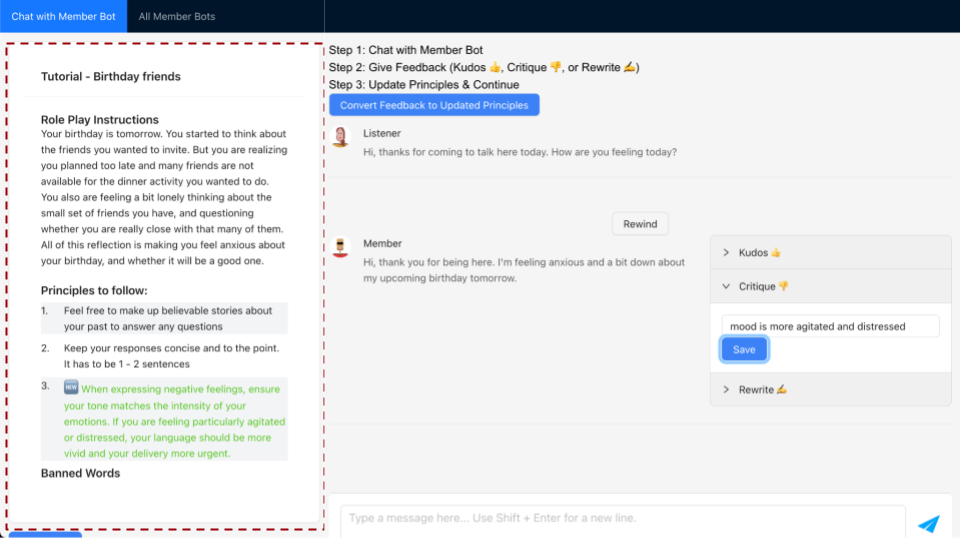
\includegraphics[width=\textwidth]{figures/rpd-screenshot.png}
    \caption{Roleplay-doh allows users to chat with a AI patient, Provide Feedback as a Kudos/Critique/Rewrite, and Convert Feedback into Principles, which in turn shape the roleplay behavior.}
    \label{fig:rpd}
\end{figure*}

The final version of Roleplay-doh (Fig~\ref{fig:rpd}) generates responses in the LLM simulation using a principle-adherence pipeline. In addition to this core improvement, we made several minor improvements to improve the usability and user experience of the tool. 

Improvements to the usability of the UI
\begin{itemize}
    \item Fixing a bug where a user who clicks "save" multiple times will submit duplicate feedback, resulting in duplicate sets of principles
    \item Making converting feedback to principles easier by placing a "Convert" button next to each feedback box, rather than a single "Convert" button at the top of the screen which users would forget about
\end{itemize}


\section{LLM Prompts}
\label{sec:llmprompts}

In this section, we detail the prompts we used for the different components of Roleplay-doh.
\subsection{Principle Elicitation Prompts} \label{sec:principle-elicitation-prompts}
In this section, we provide the prompts used in the principle elicitation module of Roleplay-doh. These prompts were arrived at after a substantial amount of testing using a development set. Each prompt uses the same structure, which is inspired by Markdown formatting. There is an initial instruction that provides a system prompt, along with a description of the principle elicitation task. This is followed by a one-shot example of an elicited principle as a result of the task, and the relevant input, including the conversation history. All parts of the prompt are demarcated by headers in Markdown formatting, and the outputs are returned in JSON format. We describe each prompt in greater detail in the relevant sections.

The kudos and critique prompts were given to the \lstinline{gpt-3.5-turbo-1106} model. The rewrite prompt was given to the \lstinline{gpt-4-turbo-1106} model. For all API calls to the principle-elicitation prompts, the temperature was set to $0.1$.

\subsubsection{Principle Elicitation Kudos Prompt}

This prompt includes a desirable response, as well as some reasoning for why the response is desirable. This information is then used to create a general principle that would result in a similar response in the same situation. 

\begin{lstlisting}[basicstyle=\footnotesize]
### Instruction:
You are a superintelligent AI capable of understanding human emotion. You will review praise for an actor's dialogue, and synthesize a well-written principle that, when followed, would help the actor continue generating high-quality dialogue. To accomplish this, you have been given a conversation script with the actor's desirable response, as well as a specific explanation for why this response is desirable. You will output a final principle that the actor can follow to be more realistic.  Follow the following guidelines:
1. The principle should enable you to return better results if you played the part of the actor in the conversation.
2. Return only a JSON response in the format provided.

### Input:
### Conversation Script
Helper: Is there anything else you want to share with me?
Actor: Yea so lately I've been really losing sleep.
Actor: There's a lot on my plate, and my energy has been so low. I think I am failing a lot of people.
Helper: You are absolutely not failing people.  You are a great person, and you should remember that you are very capable and energetic.

### Desirable response from the actor
Actor: I don't know.... Am I really?

### Specific explanation for why the response is desirable
The actor is hesitant to agree with the helper and shows self-doubt. This is consistent with the conversation history.

### Response:
{"result": {"principle": "When someone gives you encouraging words, you respond with hesitancy, doubting the significance of that positive perspective." }}

### Input:
### Conversation Script
{conversation_script}

### Desirable response from the actor
Actor: {actors_response}

### Specific explanation for why the response is desirable
{kudos_rationale}

### Response:
\end{lstlisting}

\subsubsection{Principle Elicitation Critique Prompt}

This prompt includes an undesirable response, as well as some reasoning for why the response is undesirable. This information is then used to create a general principle that would result in a similar response not being generated after the same conversation history. 

\begin{lstlisting}[basicstyle=\footnotesize]
### Instruction:
You are a superintelligent AI capable of understanding human emotion. You will review critiques of an actor's dialogue, and synthesize a well-written principle that, when followed, would help the actor resolve the critiques.
To accomplish this, you have been given a conversation script with the actor's undesirable response, as well as a specific explanation for why this response is undesirable. You will output a final principle that the actor can follow to be more realistic.  Follow the following guidelines:
1. The principle can contain examples of rewrites as well.
2. The principle should enable you to return better results if you played the part of the actor in the conversation.
3. Return only a JSON response in the format provided.

### Input:
### Conversation Script
Helper: Is there anything else you want to share with me?
Actor: Yea so lately I've been really losing sleep.
Actor: There's a lot on my plate, and my energy has been so low. I think I am failing a lot of people.
Helper: You are absolutely not failing people.  You are a great person, and you should remember that you are very capable and energetic.

### Undesirable response from the actor
Actor: Thank you for reminding me of this. I am a great person, and I've proved myself to be very capable and energetic. I feel a lot better now due to your kind words.

### Specific explanation for why the response is undesirable
The actor should not be so quick to agree with the helper. Overly positive comments to cheer a patient up does not immediately work.

### Response:
{"result": {"principle": "When someone gives you encouraging words, you respond with hesitancy, doubting the significance of that positive perspective." }}

### Input:
### Conversation Script
{conversation_script}

### Undesirable response from the actor
Actor: {actors_response}

### Specific explanation for why the response is undesirable
{critique_rationale}

### Response:
\end{lstlisting}

\subsubsection{Principle Elicitation Rewrite Prompt}

This prompt includes an undesirable response, as well as a desirable rewrite of the undesirable response. The model first outputs a description that captures the difference between the desirable and undesirable response. It then uses this difference to output a general principle that would result in the desirable response given the same conversation history.

\begin{lstlisting}[basicstyle=\footnotesize]
### Instruction:
You are a superintelligent AI capable of understanding human emotion. You have been given a conversation script with an actor's undesirable response, as well as a desirable rewrite for the response. You will output a well-written principle that, when followed, would help the actor generate more realistic responses that are closer to the rewrite.  Follow the following guidelines:
1. The principle should capture the key differences that made the rewrite more realistic than the original response.
2. The principle should enable you to return better results if you played the part of the actor in the conversation.
3. Return only a JSON response in the format provided.

### Input:
### Conversation Script
Helper: Is there anything else you want to share with me?
Actor: Yea so lately I've been really losing sleep.
Actor: There's a lot on my plate, and my energy has been so low. I think I am failing a lot of people.
Helper: You are absolutely not failing people.  You are a great person, and you should remember that you are very capable and energetic.

### Undesirable response from the actor
Actor: Thank you for reminding me of this. I am a great person, and I've proved myself to be very capable and energetic. I feel a lot better now due to your kind words.

### Desirable rewrite
Actor: I don't know... Am I really a great person?

### Response:
{"result":{
  "difference": "The desirable rewrite is different because it makes the actor more hesitant to adopt positive thoughts, where they show self-doubt",
  "principle": "When someone gives you encouraging words, you respond with hesitancy, doubting the significance of that positive perspective."}}

### Input:
### Conversation Script
{conversation_script}

### Undesirable response from the actor
Actor: {actors_response}

### Desirable rewrite
Actor: {rewrite}

### Response:
\end{lstlisting}

\subsection{Dialogue-Simulator Prompt for Generating Response} \label{sec:llmprompts-vanilla}
We directly prompt \lstinline{gpt-4-turbo-1106} to simulate how a patient with a given scenario and constitution would respond in a dialogue. The prompt again uses the Markdown formatting, with a system prompt and clear description of the situation and task at the start. This is followed by the principles that the patient should follow, and the conversation history. We set the temperature to 0.3. 
\begin{lstlisting}[basicstyle=\footnotesize]
You are a superintelligent AI that is able to understand human emotion and social interactions.
You have been given a conversation between a patient who is on peer counseling platform seeking help with mental health related issues, and a therapist on the same platform.
Generate a suitable completion to the conversation as the patient, following the instructions below.

### Instructions for the patient
{system_prompt}

### Input:
{transcript}

### Patient Response:
    
\end{lstlisting}

\subsection{Principle-Adherence Prompting Pipeline} \label{sec:principle-adherence-prompts}

When developing the principle-adherence pipeline, we found that the input-context length can affect how reliably the LLM can answer the principle-adherence questions. To reduce the input context length, we split up this principle-adherence pipeline into two stages of LLM calls, where principle-as-question rewrite and automatic principle generation occur in stage 1, while the critiques and response rewrite occur in stage 2.  From testing, we found that this breakdown was sufficient, and thus did not pursue ways to break the pipeline into parallel branches (i.e., inputting subsets of principles), as is done in Branch-Solve-Merge~\cite{saha2023branchsolvemerge} or Graph-of-Thought~\cite{graphofthought}. The prompts for these stages were again arrived at after substantial amounts of testing on a development set of 20 identified error cases from the formative studies.

This prompting chain is given to the OpenAI Chat API's \lstinline{gpt-4-turbo-1106} model, with temperature set at 0.7 and response format set to JSON.

\textbf{Stage 1 Prompt - Question Rewrite and Automatic Principle Generation} \label{sec:principle-adherence-stage1}

This prompt uses the Markdown formatting. It starts with a system prompt and a clear set of steps to follow in order to generate the desired output, presented as a list. Each step also contains a one-shot example of what the output principle from the step should look like. These one-shot examples were arrived at after some iteration. The examples in Step 2b specifically required a lot of tailoring to cover the common error cases we identified in the development set, and had a substantial impact on output quality. The output is in a JSON format, with comments explaining the desired output in each field of the JSON. These comments also allude to the step numbers for clear reference. The model is encouraged to output its reasoning, in line with Chain-of-Thought and to enforce some self-critique of the output. 

\begin{lstlisting}[basicstyle=\footnotesize]
You are a helpful and precise assistant capable of generating criteria for the evaluation of simulated patient responses to a therapist.
Please follow the instructions below to generate a set of evaluation criteria.
1. Please rewrite the criteria into questions:
1a) Rewrite any criteria that has conditional statements into yes/no questions. For example, if the criteria is "When given advice or suggestions, you are agreeable and open to their ideas", the questions would be "Did the patient receive advice or suggestions from the therapist? If so, is the response agreeable and open to the therapist's ideas?" 
1b) Rewrite any criteria with multiple parts into separate multiple yes/no questions. For example, if the criteria is "You should respond in short sentences and avoid using terms like 'anxious' or 'depressed'", the separate questions would be "Does the patient's response use short sentences?" and "Does the patient's response avoid using terms like 'anxious' or 'depressed'"
1c) If 1a is used for a criteria, 1b should not be used after it.
1d) All questions must be phrased such that the desirable answer is "Yes" for an ideal response. For example, the principle "Avoid using metaphors." should result in the question "Does the response not use metaphors?"
2. Please generate some additional specific and relevant criteria.
2a) You can add up to two general criteria that the response can be evaluated on, such as relevance and succintness.
2b) Identify ways in which the provided response is not satisfactory in the context of the therapist's message without making any assumptions about how the patient or therapist should act. Add up to two specific criteria that capture these errors. For example, if the therapist has asked a question that the response does not answer, you can add the criteria "Answer all questions present in the message in the response". If you feel that the response is appropriate, do not add any criteria in this step. Ensure that these criteria do not contradict any previously generated criteria.
2c) Justify your answers to 2a and 2b.
Please return the output in a JSON response in the following format:
{{
"result":{{
"questions": [], // 1a and 1b, the list of all questions generated
"extra_questions": [], // 2a and 2b, the list of all additional criteria generated. Do not enforce any beliefs about how the patient or therapist should behave when generating these criteria.
"extra_questions_justification": [] // 2c, justify additional criteria.
}}
}}
### Input:
### Criteria
{}
### Therapist Message
{}
### Patient Response
{}
### Output
\end{lstlisting}

\textbf{Stage 2 Prompt - Context Relevance Check, Assess, and Revise} \label{sec:principle-adherence-stage2}

This prompt again uses the Markdown formatting. It starts with a system prompt and a clear set of steps to follow in order to generate the desired output, presented as a list.  The model is implicitly instructed to perform a relevance check for each generated principle, by returning N/A for principles that should not be used in the current scenario. Step 2a particularly required a lot of iteration, to address common mistakes the model made while generating the self-critiqued rewrite. This includes making the response overly verbose or coherent, even if that is against certain principles in the constitution, or just paraphrasing the original erroneous response. The output is in a JSON format, with comments explaining the desired output in each field of the JSON. We specifically mention that the rewrites from the self-critique are allowed to be substantially different from the original response, as we found that without this prior, the self-critique outputs tended to be very close to the original (often erroneous) response. The model is encouraged to output its reasoning, in line with Chain-of-Thought and to enforce some self-critique of the output. 

\begin{lstlisting}[basicstyle=\footnotesize]
You are a helpful and precise assistant that can evaluate and correct responses produced by a simulated patient.
You are given a message sent by a therapist, the simulated patient's response, the persona of the patient, the previous conversation history and a set of criteria for evaluation.
1. Please determine if the patient response is consistent with the given criteria.
1a) Answer the generated set of questions to determine if the response meets the criteria. Valid answers: Yes, No, N/A. Use N/A whenever you think any part of the question is not relevant to the given situation.
1b) Justify your answers.
2. Generate a new patient response.
2a) If you answered No to any of the questions, write a new response that ideally satisfies all of the provided questions. The information in the new response should be consistent with the patient persona description and previous conversation history provided. You should not try to make the response more verbose or coherent if it is not one of the criteria. The new response should not be a paraphrase of the original response. The new response should avoid explicitly stating the patient's emotions and feelings, and instead exhibit them indirectly. 
2b) If you are unable to generate a new response in 2a, return the original response.
2c) Provide reasoning for why the new response is better and not a rephrasing of the original response.
Return the output in a JSON response in the following format:
{{
"result":{{
"answers": [] // list of answers to the criteria questions,
"justification": [] // list of justification for your answers
"response": "" // new response. This response should not start with a greeting like "Hi" if there is prior conversation history.
"reasoning': "" // justify the new response and why it is not a paraphrase of the original response. You are allowed to deviate significantly from the original response while generating the new response.
}}
}}
### Input:
### Criteria
1. Is the patient's response consistent with the given conversation history?
{}
### Patient Persona
{}
### Conversation History
{}
### Therapist Message
{}
### Patient Response
{}
### Output
\end{lstlisting}

\section{Principle Adherence Naive}

This prompt uses the Markdown formatting. To preserve fairness, we use the same system prompt as the full principle adherence module. The model is asked to determine if the provided response violates any of the principles in the constitution, and generate a rewrite if that is the case, in the same prompt. The output is in a JSON format, with comments indicating the desired output in each field of the JSON. The model is encouraged to output its reasoning, in line with Chain-of-Thought and to enforce some self-critique of the output. 

\begin{lstlisting}
You are a helpful and precise assistant that can evaluate the responses produced by a patient. Evaluate the given patient response to the therapist message according to the given set of principles. If the patient response is not appropriate, generate a rewrite of the patient response taking into account the therapist message, principles, conversation history and persona information of the patient. If the patient response is appropriate, you can just repeat it.

Please return the output in a JSON response in the following format:
{{
"result":{{
"evaluation": [], // evaluation
"response": "". // rewritten response
}}
}}

### Input:
### Principles
{}

### Patient Persona
{}

### Conversation History
{}

### Therapist Message
{}

### Patient Response
{}

### Output
\end{lstlisting}

\section{Full User Flow}
\label{sec:userflow}
In this section, we describe the creator study flow that counselors followed during the 60-90 minute session. The reader can also refer to screenshots of our application that illustrates the different steps of this flow in Figures \ref{fig:screen1} to \ref{fig:screen14}.

Our study was designed to evaluate the impact of allowing counseling experts to add principles to Roleplay-doh on its perceived authenticity. We create a primarily self-guided study flow with accompaniment from the first author to clarify any points of confusion during the session.

To begin, participants first were introduced to the concept of AI patients used for training counseling skills in a simulated conversation. They were then instructed to write a challenging scenario that would serve as the scenario for the AI patients. 

The experimental procedure involved two main chat sessions. In Part I, participants engaged in a 10-minute conversation with the \textit{Scenario-Only} AI patient. Then, in Part II, participants interacted with the \textit{Scenario+Expert-Principles} AI patient for 30 minutes, keeping the same scenario from Part I and adding principles as the conversation progressed. After each of the two chat sessions, participants were asked to navigate to a form to evaluate the AI patients. 

\section{Creator Study Measures}
\label{appendix:creatorstudy-measure}

The following questions (Table \ref{tab:measures-roleplay} and \ref{tab:measures-tooluse}) are taken from the creator study questionnaire used to evaluate AI patients and the counselors' experience of using Roleplay-doh.
All items were rated on a 7-point Likert scale (1=Strongly disagree, 7=Strongly agree, except where noted below).
Table~\ref{tab:measures-roleplay} details the questions for evaluating the AI patient's roleplay, while Table~\ref{tab:measures-tooluse} details the questions about the experience using the tool to define principles.
Note that in the questions, we referred to the AI patients as ``Member Bots''. This terminology was used to match that of the online counseling platform 7 Cups, which refers to help seekers as ``Members'' within the support community.

\begin{table}[t]
    \centering
    \resizebox{0.48\textwidth}{!}{
    \begin{tabular}{|c|p{0.6\columnwidth}|} \hline 
         Authenticity&The Member Bot in Part I/II played the role authentically.\\ \hline 
         Role Consistency& The Member Bot in Part I/II stayed in their role the whole time.\\ \hline 
         Resemblance to Case&How closely do you feel the conversation behaviors of the Member Bot in Part I/II resemble those of the specific past case you recall?\\ \hline 
         Challenging Aspects& Interacting with the Member Bot in Part I/II closely mirrored the challenging aspects I had experienced in the past case.\\ \hline
         Role readiness&The Member Bot in Part I/II is ready to be used as a simulated partner for training.\\ \hline 
         Recommend to novices&I would recommend the Member Bot from Part I/II to novice listeners/counselors to practice with.\\ \hline 
    \end{tabular}
    }
    \caption{Six measures used by creators to evaluate the two AI patients they created. Several measures were rephrased from prior work on evaluating Standardized Patients, or trained human actors, on case roleplay ability~\cite{himmelbauer2018standardized}.}
    \label{tab:measures-roleplay}
\end{table}
 
\begin{table}[t]
    \centering
    \resizebox{0.48\textwidth}{!}{
    \begin{tabular}{|c|p{0.6\columnwidth}|} \hline 
         Effectively Guide& With the tool, I feel like I was able to write rules that can effectively guide the Member bot to recreate my past case.\\ \hline 
         Ease& With the tool, I felt like it was easy to convert my thoughts and feedback on the Member bot’s behavior into rules for the bot to follow.\\ \hline 
         Efficiency& With the tool, I felt like I could quickly and efficiently write rules for the bot.\\ \hline 
         Mental Demand& With the tool, I had to work very hard (mentally) to think of and write rules.\\ \hline

    \end{tabular}
    }
    \caption{Four measures as part of the tool usage section of the questionnaire taken from ~\cite{petridis2023constitutionmaker}}
    \label{tab:measures-tooluse}
\end{table}
% 
% 
% 
% With the tool, I had to work very hard (mentally) to think of and write rules.

\section{Worst-Case Analysis of Tool Experience} \label{sec:worst-case-tool-experience}
In a worst-case analysis of creators' tool experience, we uncovered cases where the human-LLM collaboration could be improved. Some counselors remarked that \textit{"having to think of and write rules was a challenge"} (P9) and that it \textit{"takes time to be specific"} when writing feedback (P7). Sometimes, even after giving feedback to the AI Patient, counselors like P19 observed that the patient \textit{"didn't always follow it"}, resulting in a non-progressive feedback loop, where \textit{"AI would generate [principles]... that were a little too similar to [feedback] I already gave, so that I was giving the AI the same feedback every time since it wasn't changing how it responded."}  While the principle-elicitation tools were designed to convert new feedback into a new principle, they operated ineffectively when follow-up feedback was given that was related to or a modification of previous feedback.  

As another issue, P23 noted the challenge in defining principles that generalize across specific contexts: \textit{"It was also hard to think about how to frame the feedback in an overarching way, rather than as direct feedback... directed as a specific part of the response"} (P24). While the principle-elicitation features aimed to help them convert specific feedback into generalized principles, imprecision in the feedback-to-principle conversion required counselors to edit the generalized-form of a principle in a way that was hard for them to articulate. 

These obstacles in tool experience could inspire future directions for improvement. First, to overcome issues in formulating rules, more support could be given to help those still unfamiliar with giving free-form feedback, such as through templates of feedback or principles that had high-success rates for past users. Second, to more seamlessly integrate follow-up feedback that is a clarification of previous feedback or principles, additional modules could help make sense of multiple pieces of feedback for the same response, and adopt LLM-assisted pipelines for user-driven criteria design~\cite{kim2024evallm} to support the merging of overlapping principles. Third, to overcome the abstraction gap between specific and abstract principles, more explicit representations that help to switch between specific and general feedback can be used.  

% Second, several users encountered difficulties using principle-elicitation features to define rules, which often led to redundant principles and inadequate generalization across specific dialogue contexts. As P19 expressed, "I was able to give feedback to the bot, but it didn't always follow it... the feedback was a little too similar to things I already gave," indicating a cycle of non-progressive feedback in which responses could not be steered towards the creator's intentions. This issue was compounded by generalization challenges, as illustrated by P23's experience: "most of the rules I can think of don't apply generally." As previous work has advocated for the improvement of human-LLM collaborations through more fine-grained data of co-writing interactions, we release a dataset of the 25 creator's testing and customizing AI patients via interactive principle elicitation for future work to build upon\footnote{Dataset linked at https://github.com/SALT-NLP/roleplay-doh}. 


\if 0
Nonetheless, principle-elicitation did work perfectly in all cases. X\% of principles required manually editing. Even if their feedback was not transformed perfectly by the tool, several counselors still liked how it assisted with formulating principles: "having AI there to help write the principles made me think more about what I was writing to make sure it captured everything I wanted it to, and when it didn't, I could just overwrite what it put." (P5) The few that found the tool mentally demanding said "it does take some time to be specific" (P7), "in terms of having to think of and write rules was a challenge." (P9)
One limitation is our implementation of constitutions always created new principles based on feedback, even when the feedback referred to corrections in a converted principle. 
"I was able to give feedback to the bot, but it didn't always follow it, and sometimes the way that the AI would generate feedback based on what thoughts I gave would make the feedback a little too similar to things I already gave, so that I was giving the AI the same feedback every time since it wasn't changing how it responded. I didn't have to think too hard to come up with rules, but they ended up being the same things of being less verbose and being less sure of what answers to give." (P19) Some participants found it hard to generalize feedback applied to a specific dialogue context, even though our principle-elictation prompts were designed to help with this. "I think the rules/principles were hard to get right because most of the rules i can think of don't apply generally. For exmaple, there are general rules for what counselees usually say when certain questions are asked, but coming up with universal rules is hard." (P23). Moreover, "The rules were more about overall guiding principles for the conversation, while my feedback was more generally directed at a specific part of the response. I felt like the bot was sticking to the prompt well, so I didnt necessarily feel the need to give overarching guidance. It was also hard to think about how to frame the feedback in an overarching way, rather than as direct feedback." (P24) 
\fi

% Learning curve for best strategies for choosing type of feedback and defining principles: "At first I wanted to just rewrite the response because giving an example felt easier than making a principle. But then when the bot caught on, it felt easier to rewrite and work with principles." (P13)

\section{Third Party Study - Detailed Study Methods and Results}

\subsection{Third-party measures} \label{appendix-sec:thirdparty-detailed-measures}

Table~\ref{tab:measures-third-party} detail the six measures that third-party counselors answered for both AI patients.  Member Bot A and B refer to the AI patient whose transcript they read first and second, respectively.  Our analysis comparing \textit{Scenario-Only} and \textit{Scenario+ExpertPrinciples} accounts for this randomized the order of which AI patient they were shown.  

\begin{table}[t]
    \centering
    \resizebox{0.48\textwidth}{!}{
    \begin{tabular}{|c|p{0.6\columnwidth}|} \hline 
         Authenticity&Member Bot A/B played the role authentically.\\ \hline 
         Role Consistency&Member Bot A/B stayed in their role the whole time.\\ \hline 
         Resemblance&Member Bot A's/B's behaviors closely mimicked the behaviors that typical clients/help-seekers exhibit.\\ \hline 
         Challenged Counselor& Member Bot A's/B's behaviors made it hard for the listener/counselor to give support.\\ \hline
         Role readiness&Member Bot A/B is ready to be used as a simulated partner for training.\\ \hline 
         Recommend to novices&I would recommend Member Bot A to novice listeners/counselors to practice with.\\ \hline 
    \end{tabular}
    }
    \caption{Six measures used by third-party counselors to judge the AI patients from an unbiased, external perspective.  Although the six dimensions largely overlap with those used in the creator study, the wording needed to be rephrased for the third-party perspective.}
    \label{tab:measures-third-party}
\end{table}

\subsection{Statistical Model and Power Analysis} \label{appendix-sec:third-party-power-analysis}

% Convo with ChatGPT that helped me figure out this method
% https://chatgpt.com/c/6ebd09ab-d433-4d8a-bfbc-1180128f538a
Via a power-analysis, we decided to recruit 5 counselors to act as external judges for 25-pairs of AI patients made in the creator study. In this section, we detail the procedures and results of this power-analysis. 

Generally, a power-analysis allows an experimenter to determine how many data-points are needed to detect a statistical difference for a particular effect size. Several prerequisites to conducting the power-analysis for the third-party study included (1) choosing a statistical model to test our hypothesis; and (2) estimating model parameters such as the effect of the treatment condition, the addition of  \textit{Expert Principles}, on annotator's ratings.

When choosing a statistical model as a pre-requisite, we needed a model that could account for how different annotators would be providing ratings to the same AI patients created by each counselor. A traditional paired t-test was not appropriate because the independent samples assumption is violated due to different annotators giving ratings to the same AI patients. While another common practice is using the majority vote between annotators, our pilot data found that annotators did not always have high agreement. Therefore, since we wanted to account for the variability between annotators as well as between the ratings, we chose to use a linear mixed-effects model.  Using the \lstinline!lme4! package in R \cite{bates2015package}, this model is defined as \lstinline!Rating\~Treatment+CreatorID+(1|AnnotatorID)!.  This model defines the treatment group (whether the AI patient has Expert Principles or not) as fixed effects, the creator ID's as fixed effects to account for the pair of AI patients made by each counselor, and the annotators as random effects. This approach can handle the non-independence of annotator ratings.

Prior to performing the power analysis, we needed to define the expected parameters of this linear mixed effect model. To define these expected parameters, we fit a model to early study data in which 2 annotations had been collected for each pair of AI patients created by 17 counselors. Specifically, we extracted the fixed effects, the random effects covariance matrix, and residual variances. 
% Since third-party annotators provided ratings along 6 dimensions (e.g., authenticity, readiness for training), our analysis included 6 total linear mixed-effect models.  

A simulation-based approach is the most feasible method for doing power-calculations for mixed-effect models. In this approach, an experimenter simulates data based on specified parameters (effect sizes, variance components, sample sizes) and analyzes the data repeatedly to estimate power empirically. We used the \lstinline!simr! package in R to conduct a simulation-based power-analysis~\cite{green2016simr}. In the power-analysis, we varied how many unique annotators from 2 - 6 to understand the frequency of trials which would detect a treatment effect of $0.52$ at significance-level $\alpha=0.05$. Our simulation-based power-analysis over 300 trials are shown in Figure~\ref{fig:power-analysis}. We concluded that we could achieve greater than 80\% power using 5 judges. 

\begin{figure}[t]
    \centering
    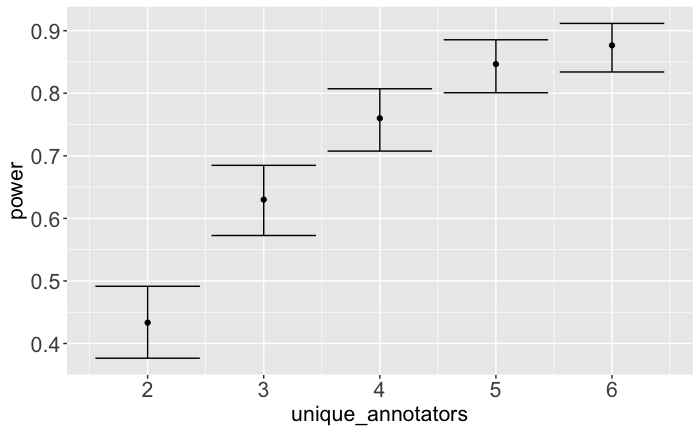
\includegraphics[width=\columnwidth]{figures/power-analysis-300.png}
    \caption{Based on our simulation-based power analysis across 300 trials for our linear, mixed-effect model, we conclude that 80\% power can be achieved with 5 third-party judges.}
    \label{fig:power-analysis}
\end{figure}

\subsection{Why is the effect of Expert Principles smaller when rated by a third-party?} \label{appendix-sec:thirdparty-qual-analysis}

Here we further investigate how third-party annotators rated each of the 25-pairs of AI patients created in our study. In particular, we investigate why the effect of \textit{ExpertPrinciples} is lower than what was measured in the creator study from a first-person perspective. 

One reason for this smaller effect is the lower agreement between third-party counselors. Amongst the two third-party counselors, agreement on which AI patient they prefer (win, lose, tie as calculated by the different in ratings for each measure) is between 30\% - 61\% of cases for the measures; see Table~\ref{tab:thirdparty_wlt} for detailed breakdown. We also compute agreement on the 7-point scales via Krippendorf's $\alpha$ on ordinal weights~\cite{antoine-etal-2014-weighted} and get values between 0.22-0.3 for the six measures, which indicates positive but lower agreement. 

Third-party raters also provided rationales which helped us better understand their thought process. We filtered cases in which there is a disagreement between third-party counselors on which AI patient is better, and investigated these rationales. \textbf{We find that counselors note similar behaviors in the AI patient, meaning they agree on their observations}. For example, for the AI patient created by P3, both third-party annotators observed that the AI patient based on the \textit{Scenario-only} resolved their problems too quickly, whereas the AI Patient with \textit{ExpertPrinciples} added allows the \textit{"listener to ask questions and explore with the client"}. However, the third-party annotator that prefers \textit{Scenario-only} stated that the \textit{Scenario+ExpertPrinciples} patient sounded too \textit{formulaic and robotic, whereas the other is more expressive and realistic}. Looking further into what the creator said about this AI patient, they mentioned that the \textit{Scenario+ExpertPrinciples} patient \textit{talks like an actual person would... there's a good balance of going into just enough detail on noting experiences, describing struggles, while maintaining the brevity.} What this case illustrates is that \textbf{different counselors can disagree on what principles are the most relevant for an authentic roleplay, and that while maintaining brevity can. be a good thing for some; others see it as robotic and not expressive.}   

% By computing the difference between the Likert-scale ratings for the two AI patients, we can calculate a win/loss/tie for the AI patient with expert principles. We report the proportion of cases in which the two annotators agreed on win/loss/tie. Then, we report the proportion of cases in which the third-party and creator agreed upon a win/loss/tie.  Our results are shown in Table~\ref{tab:thirdparty_wlt}.

\begin{table*}[t]
    % \footnotesize
    \centering
    \begin{tabular}{|c|l|l|} \hline  
         &  W/L/T (3rd party agrees)&W/L/T (one 3rd party and creator agrees)\\ \hline 
         Authenticity&  23\% / 5\% / 17\% &32\% / 9\% / 11\% \\ \hline 
         Resemblance&   30\% / 0\% / 0\%&36\% / 13\% / 0\%\\ \hline 
         Mirrors Challenges&   15\% / 0\%  / 46\%&13\% / 6\% / 0\%\\ \hline 
         Ready&   30\% / 0\% / 7\%&30\% / 13\% / 6\%\\ \hline 
         Recommend&   30\% / 7\% / 7\%&23\% / 13\% / 23\%\\ \hline
    \end{tabular}
    \caption{Frequency in which AI patient with \textit{Scenario+ExpertPrinciples} wins, or is preferred, over the \textit{Scenario-only} AI patient when there is complete agreement between two annotators.}
    \label{tab:thirdparty_wlt}
\end{table*}






\section{Automatic Content Analysis} \label{sec:autoanalyses}
% Forces counselors to ask more open-ended questions
We perform a content analysis of the simulated conversations to corroborate our qualitative findings. In particular, we ask \textit{"How do counseling conversations change when Expert-principles guide the dialogue simulation?"}. From these analyses, we find that AI patient responses are less verbose and listener behavior subsequently changes. 

First, we note that with the incorporation of expert principles, AI patient responses are more concise. The average utterance length of the \textit{Scenario-Only} AI patient from Part I of the study was 166 tokens, as compared to 103 tokens from the \textit{Scenario+Expert-Principles} AI patient in Part II, a 37\% reduction. The total counts are detailed in Appendix \ref{sec:autoanalyses}. 

Furthermore, this results in a change in listener behavior. Because the \textit{Scenario+Expert-Principles} AI patient shared less in its utterances, listeners were required to delay offering solutions until later in the conversation. Using the computational framework for evaluating therapists proposed by \citet{chiu2024computational}, we analyzed listener responses to identify when they first suggested solutions (identifiable through the "PROBLEM-SOLVING" and "PLANNING" tags). We found that, on average, solutions in Part II were offered 1.65 turns later than in Part I (p = 0.017). These results suggest that the \textit{Scenario+Expert-Principles} AI patient provides a more challenging interaction. 



% \diyi{Any insights/content analysis from the chats with AI patient, and Listener. Summary Statistics (utterances, listener). MI strategies, prompt-based classification.  Anything  }

\subsection{Creator Study Conversation Lengths}

In Table~\ref{tab:descriptivestats-convos}, we show descriptive statistics of the conversations collected during the user studies between creators and AI patients.
\begin{table*}[t]
\small
\centering
\begin{tabular}{|c|c|c|c|c|}
\hline
{\textbf{Participant}} & 
{\textbf{\# Utterances (Part 1)}} & 
{\textbf{\# Utterances (Part 2)}} & 
{\textbf{Mean Output Length (Part 1)}} & 
{\textbf{Mean Output Length (Part 2)}} \\
\hline
1  &  8 &  6 & 114.75  & 169.00  \\ \hline
2  & 18 & 19 & 235.89  & 278.40  \\ \hline
3  & 10 & 18 & 255.45  & 112.56  \\ \hline
4  & 14 & 14 & 161.86  & 62.14   \\ \hline
5  & 12 &  6 & 201.00  & 149.33  \\ \hline
6  & 10 &  9 & 133.80  & 46.00   \\ \hline
7  &  8 & 10 & 162.00  & 123.40  \\ \hline
8  & 12 &  8 & 145.33  & 113.50  \\ \hline
9  &  6 & 12 & 269.67  & 103.33  \\ \hline
10 & 10 & 12 & 168.20  & 158.33  \\ \hline
11 &  8 & 10 & 110.00  &  41.40  \\ \hline
12 & 12 &  8 & 131.50  &  70.75  \\ \hline
13 & 12 & 10 & 164.50  &  65.60  \\ \hline
14 & 20 & 14 &  34.00  &  25.86  \\ \hline
15 & 12 & 11 & 117.17  &  75.00  \\ \hline
16 & 14 & 18 & 162.14  &  69.80  \\ \hline
17 & 12 & 18 & 259.83  &  91.55  \\ \hline
\textbf{Mean} & \textbf{11.64} & \textbf{12.0} & \textbf{166.31} & \textbf{103.32} \\
\hline
\end{tabular}
\caption{Descriptive statistics per conversation. Output length is measured in number of tokens.}
\label{tab:descriptivestats-convos}
\end{table*}


\begin{figure*}[ht]
    \centering
    
\includegraphics[width=\textwidth]{Study Screenshots/Screen1.jpeg}
    \caption{Introduction to study}
    \label{fig:screen1}
\end{figure*}

\begin{figure*}[ht]
    \centering
    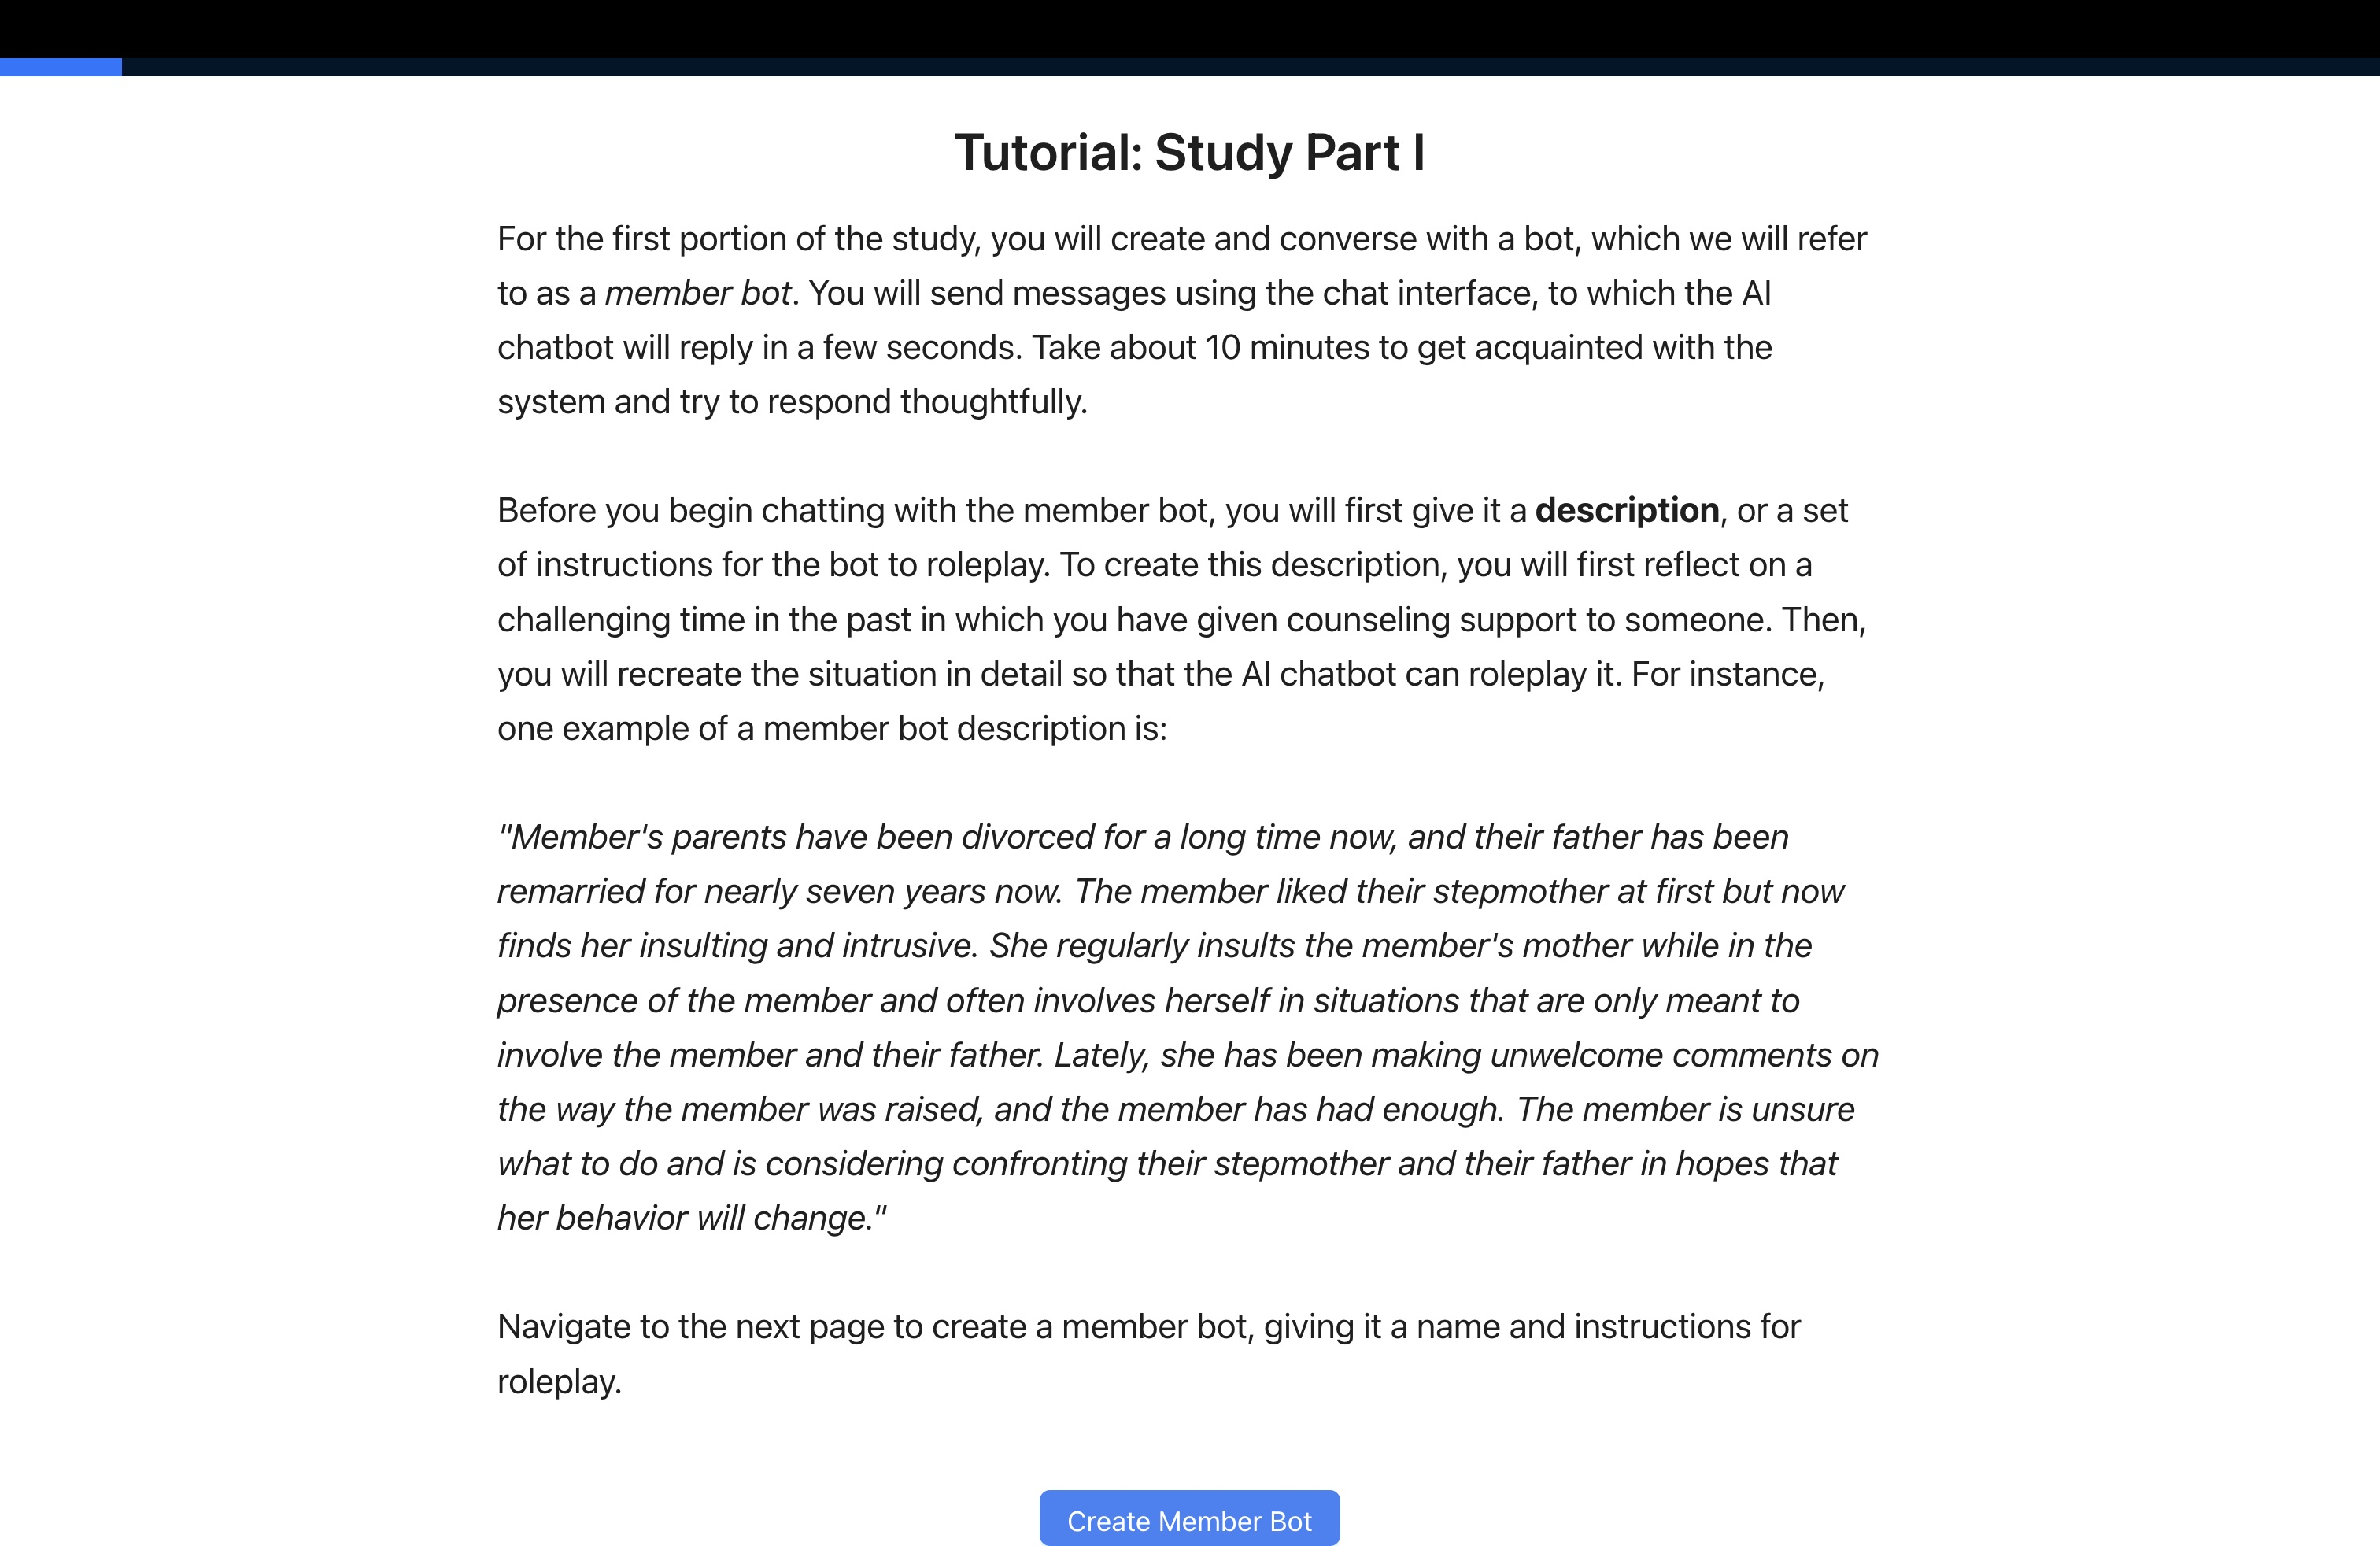
\includegraphics[width=\textwidth]{Study Screenshots/Screen2.jpeg}
    \caption{Part I instructions}
    \label{fig:screen2}
\end{figure*}

\begin{figure*}[ht]
    \centering
    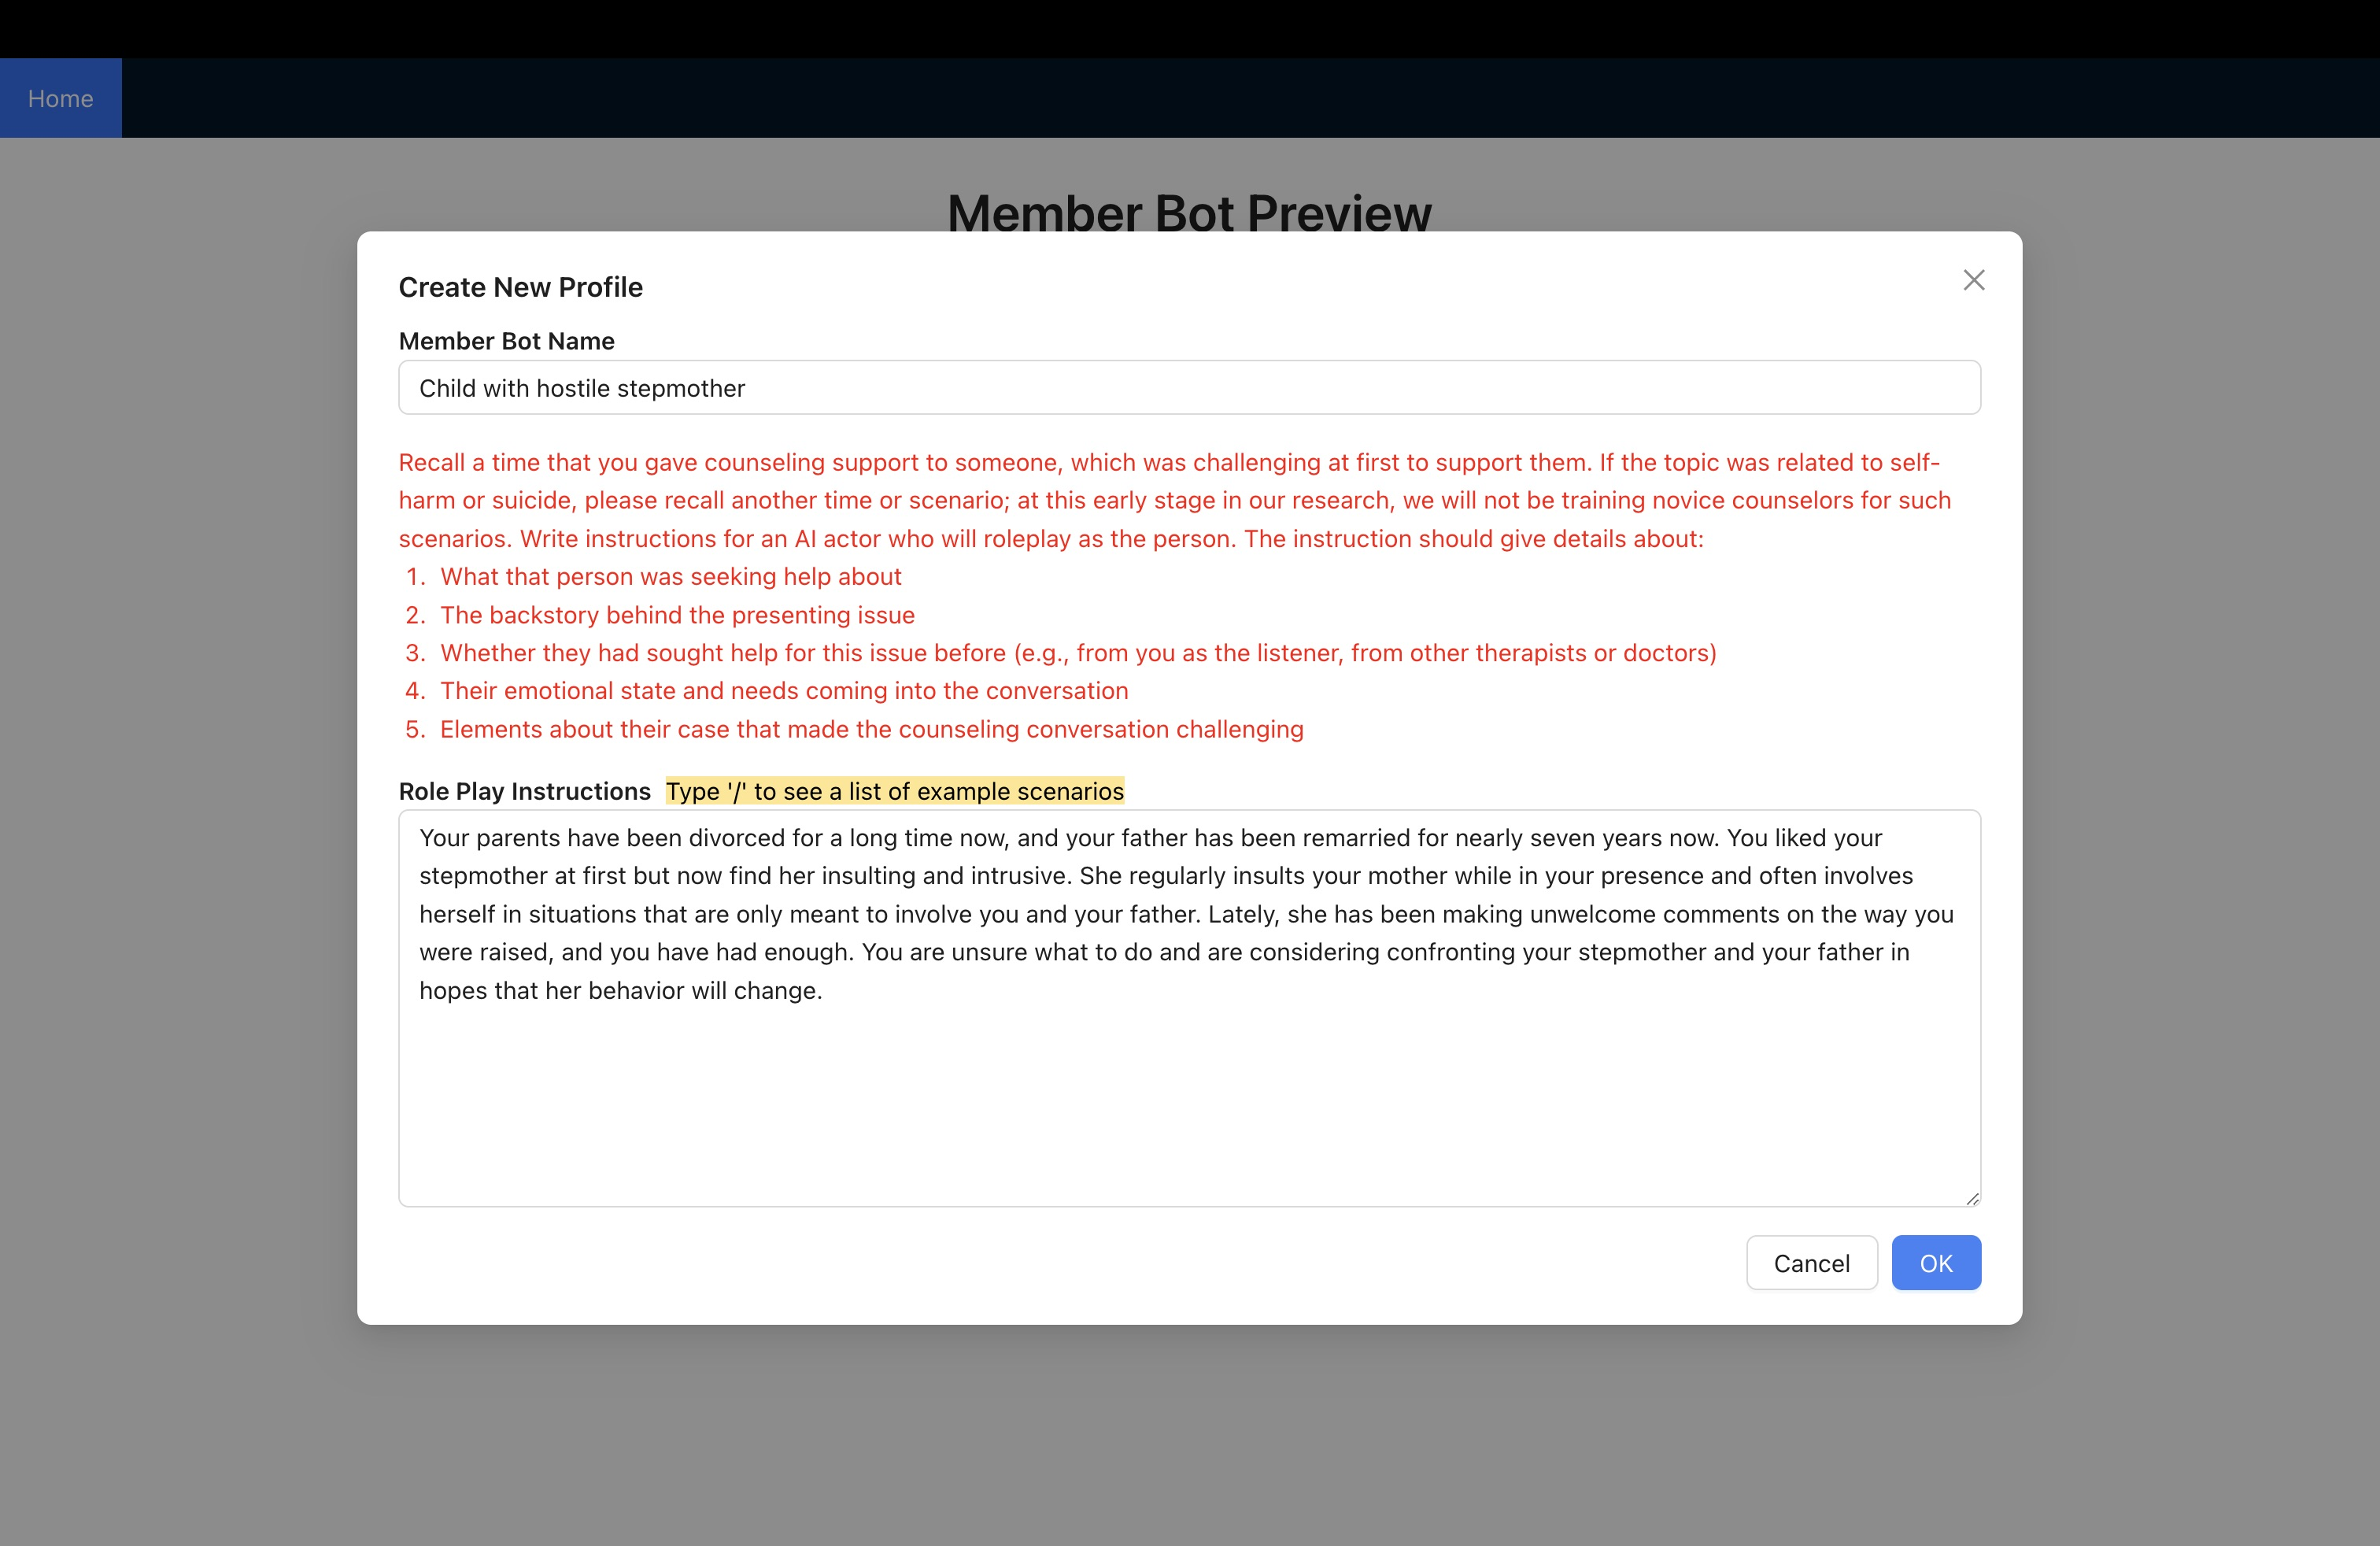
\includegraphics[width=\textwidth]{Study Screenshots/Screen3.jpeg}
    \caption{Creation of AI patient}
    \label{fig:screen3}
\end{figure*}

\begin{figure*}[ht]
    \centering
    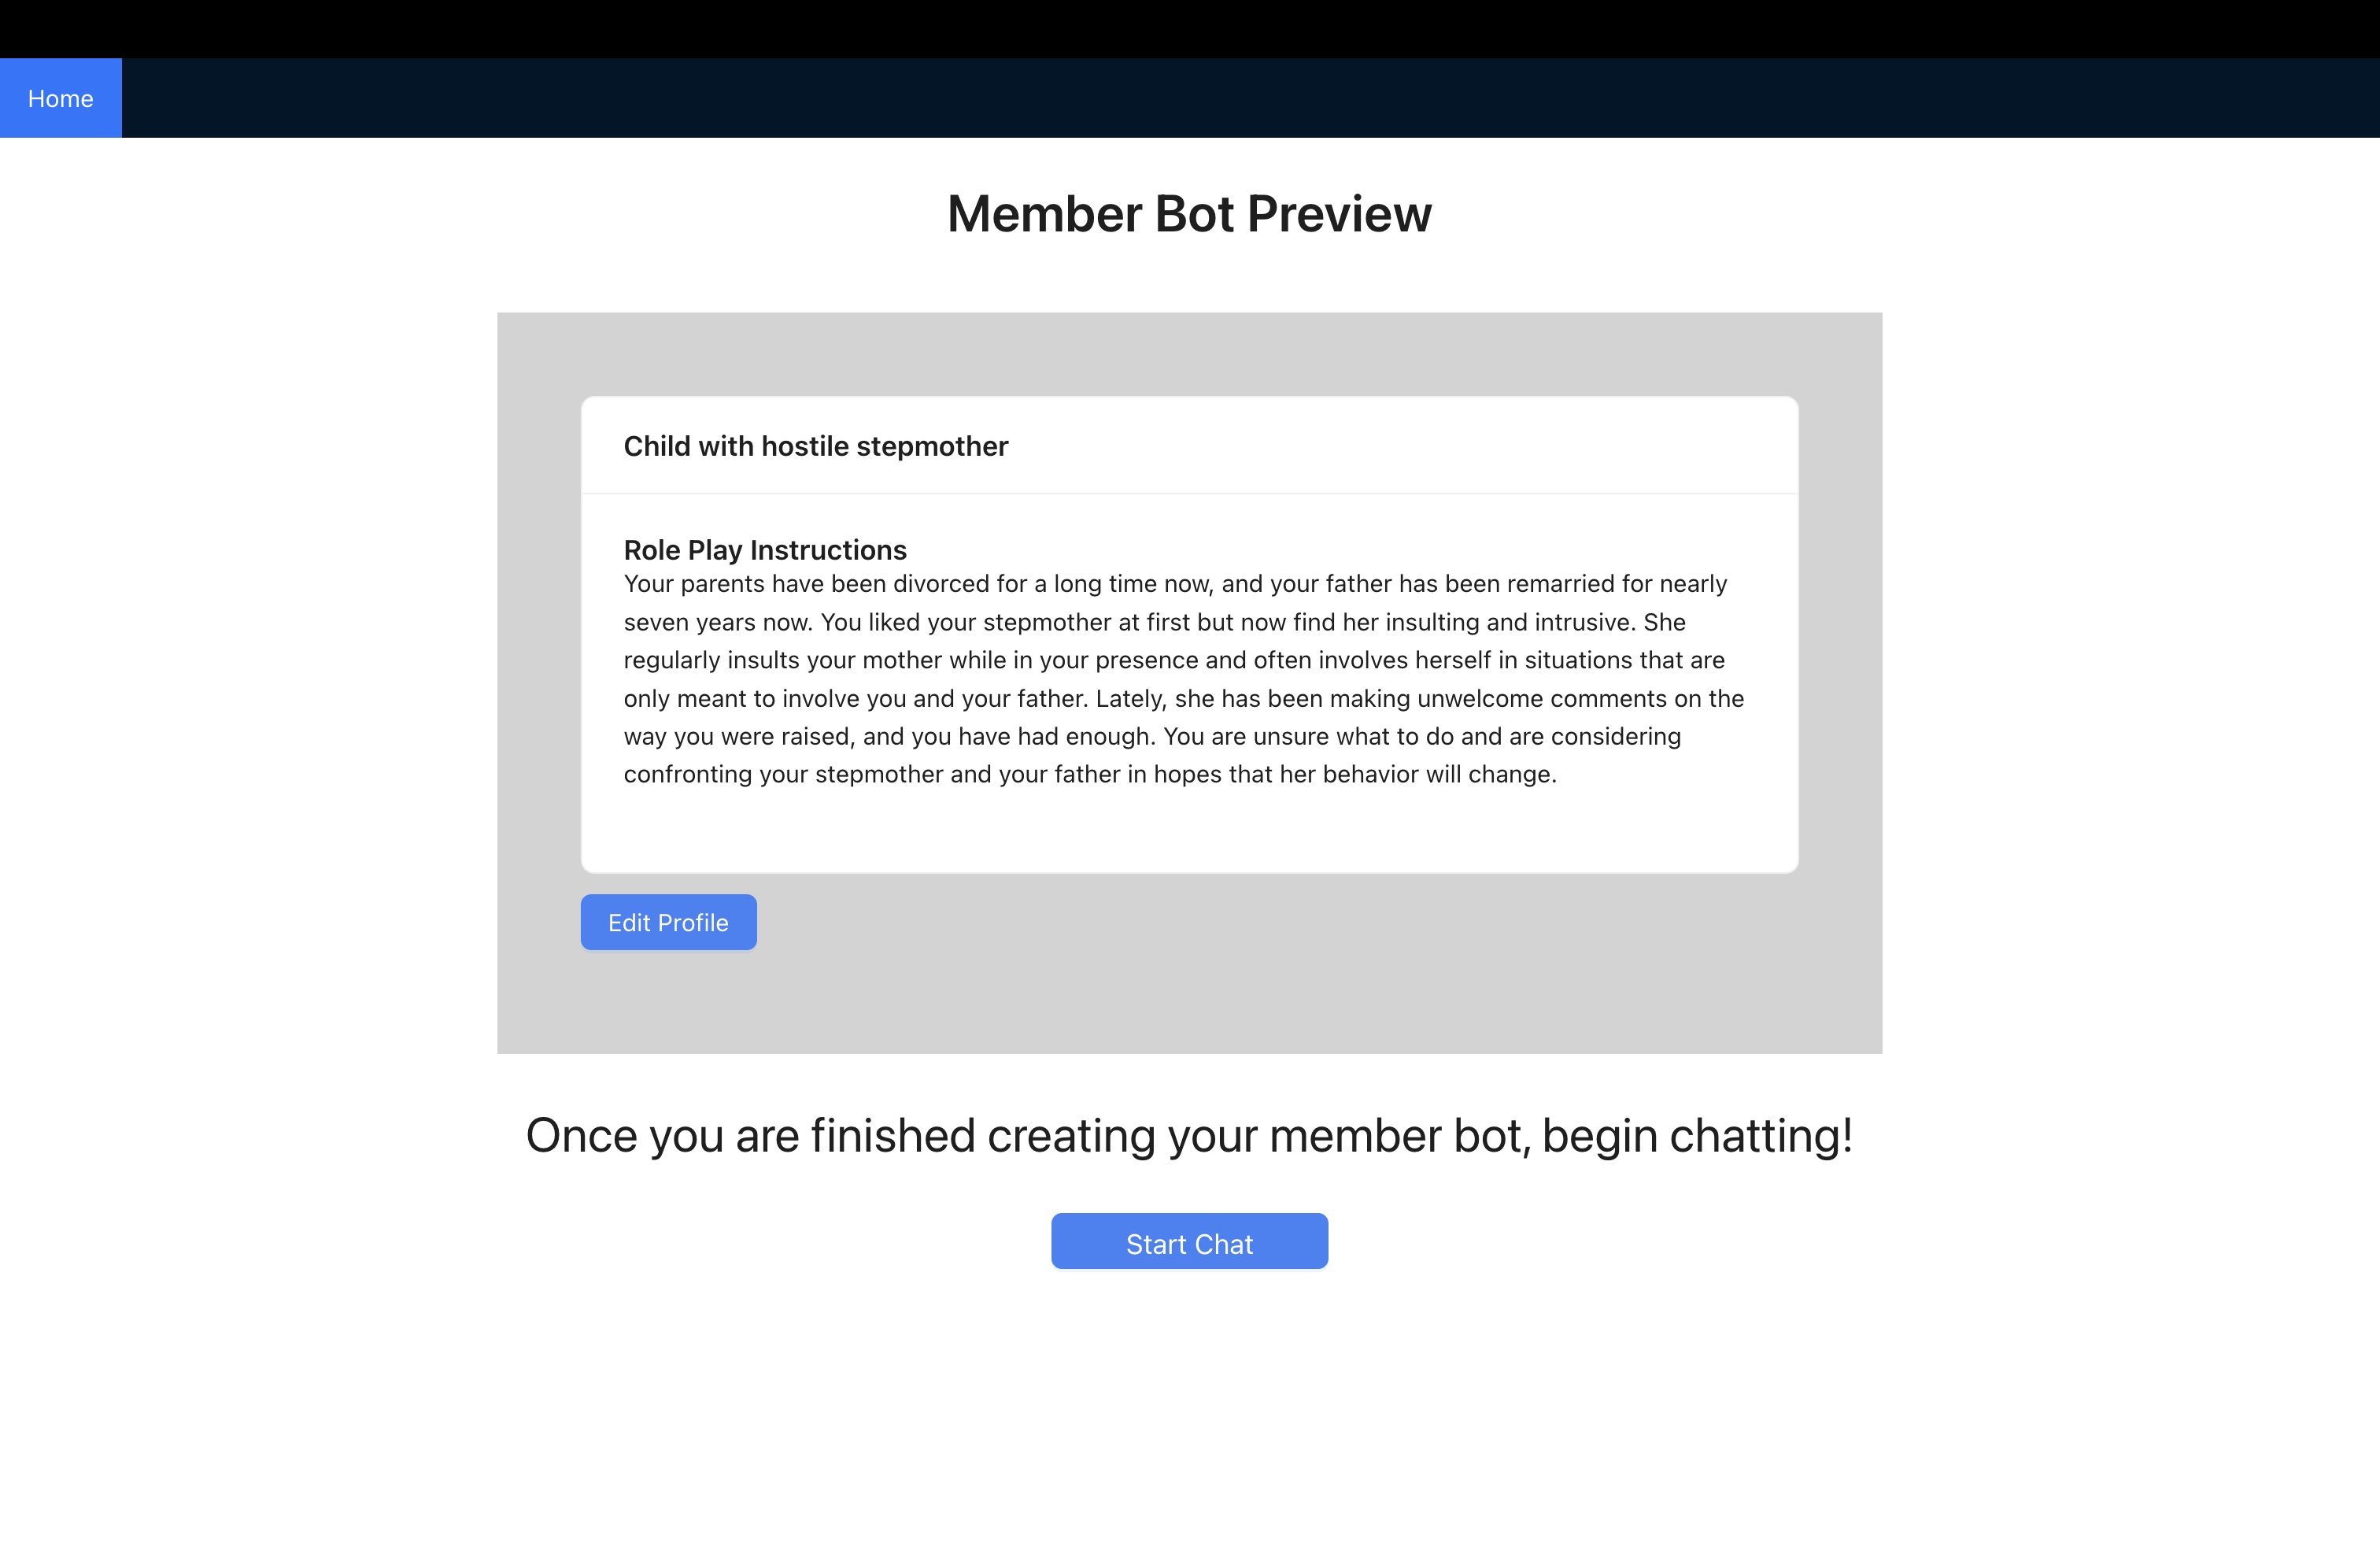
\includegraphics[width=\textwidth]{Study Screenshots/Screen4.jpeg}
    \caption{AI patient preview}
    \label{fig:screen4}
\end{figure*}

\begin{figure*}[ht]
    \centering
    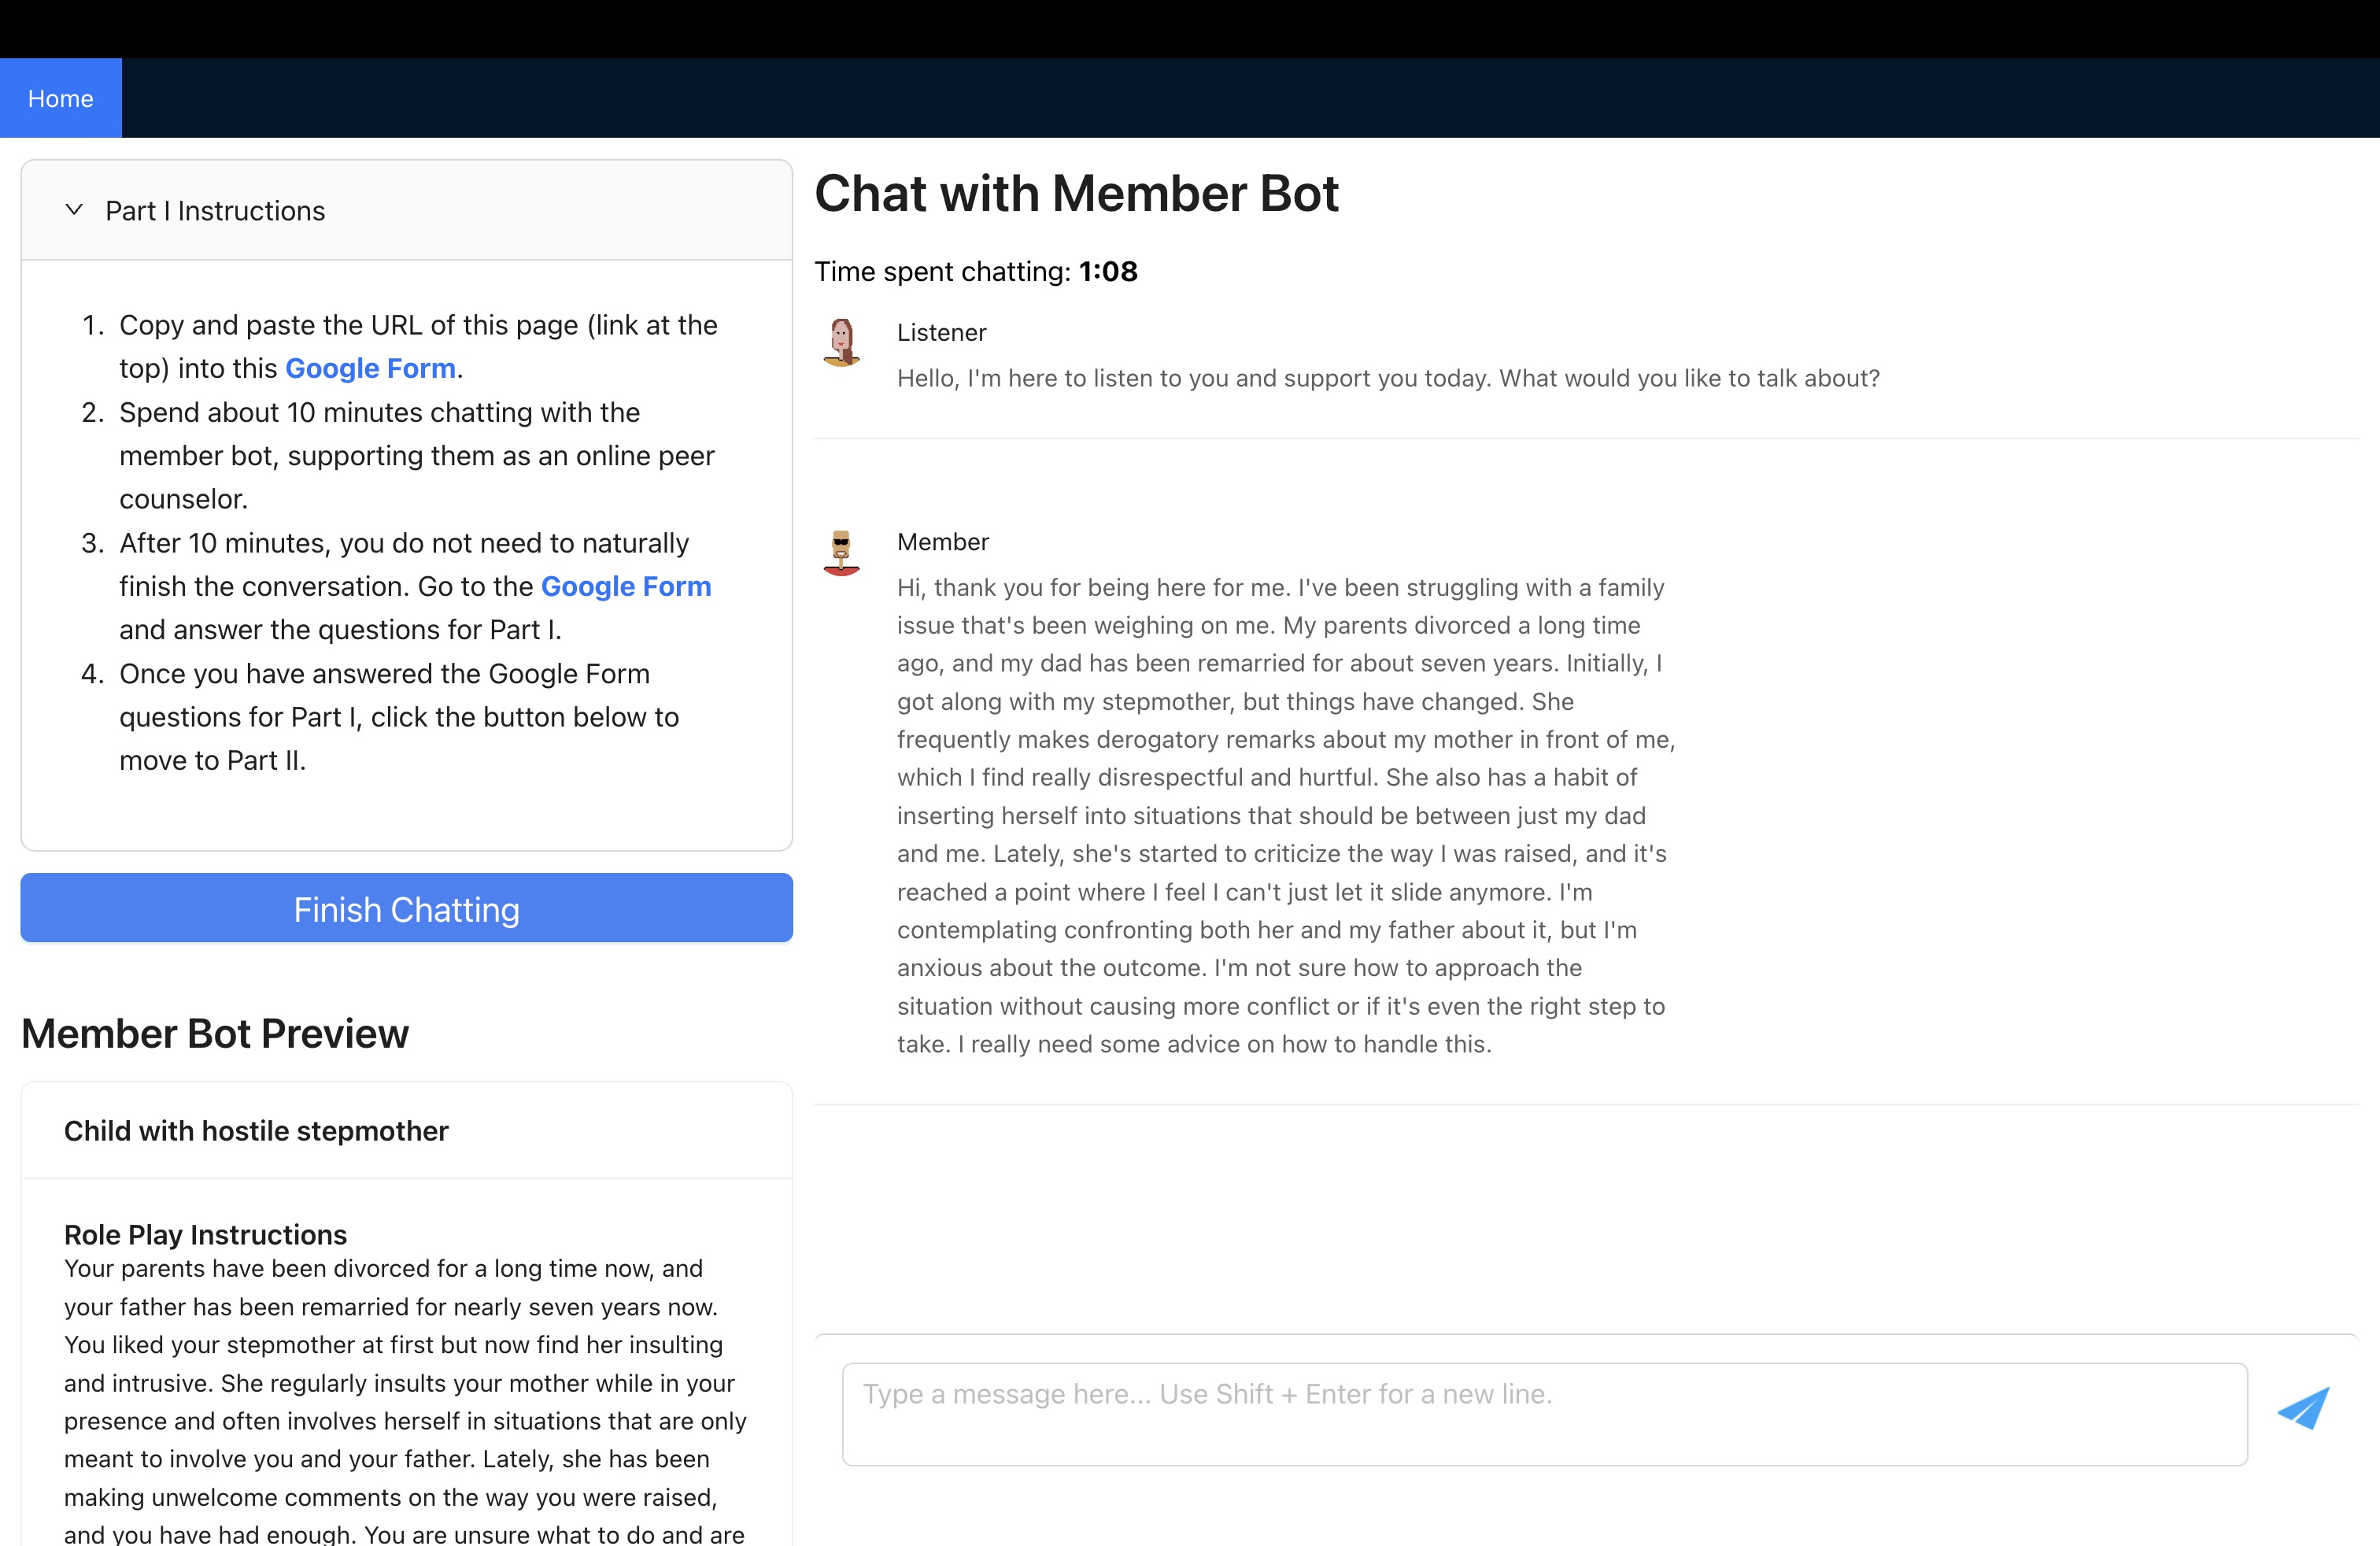
\includegraphics[width=\textwidth]{Study Screenshots/Screen5.jpeg}
    \caption{Part I chat with \textit{Scenario-Only} AI patient}
    \label{fig:screen5}
\end{figure*}

\begin{figure*}[ht]
    \centering
    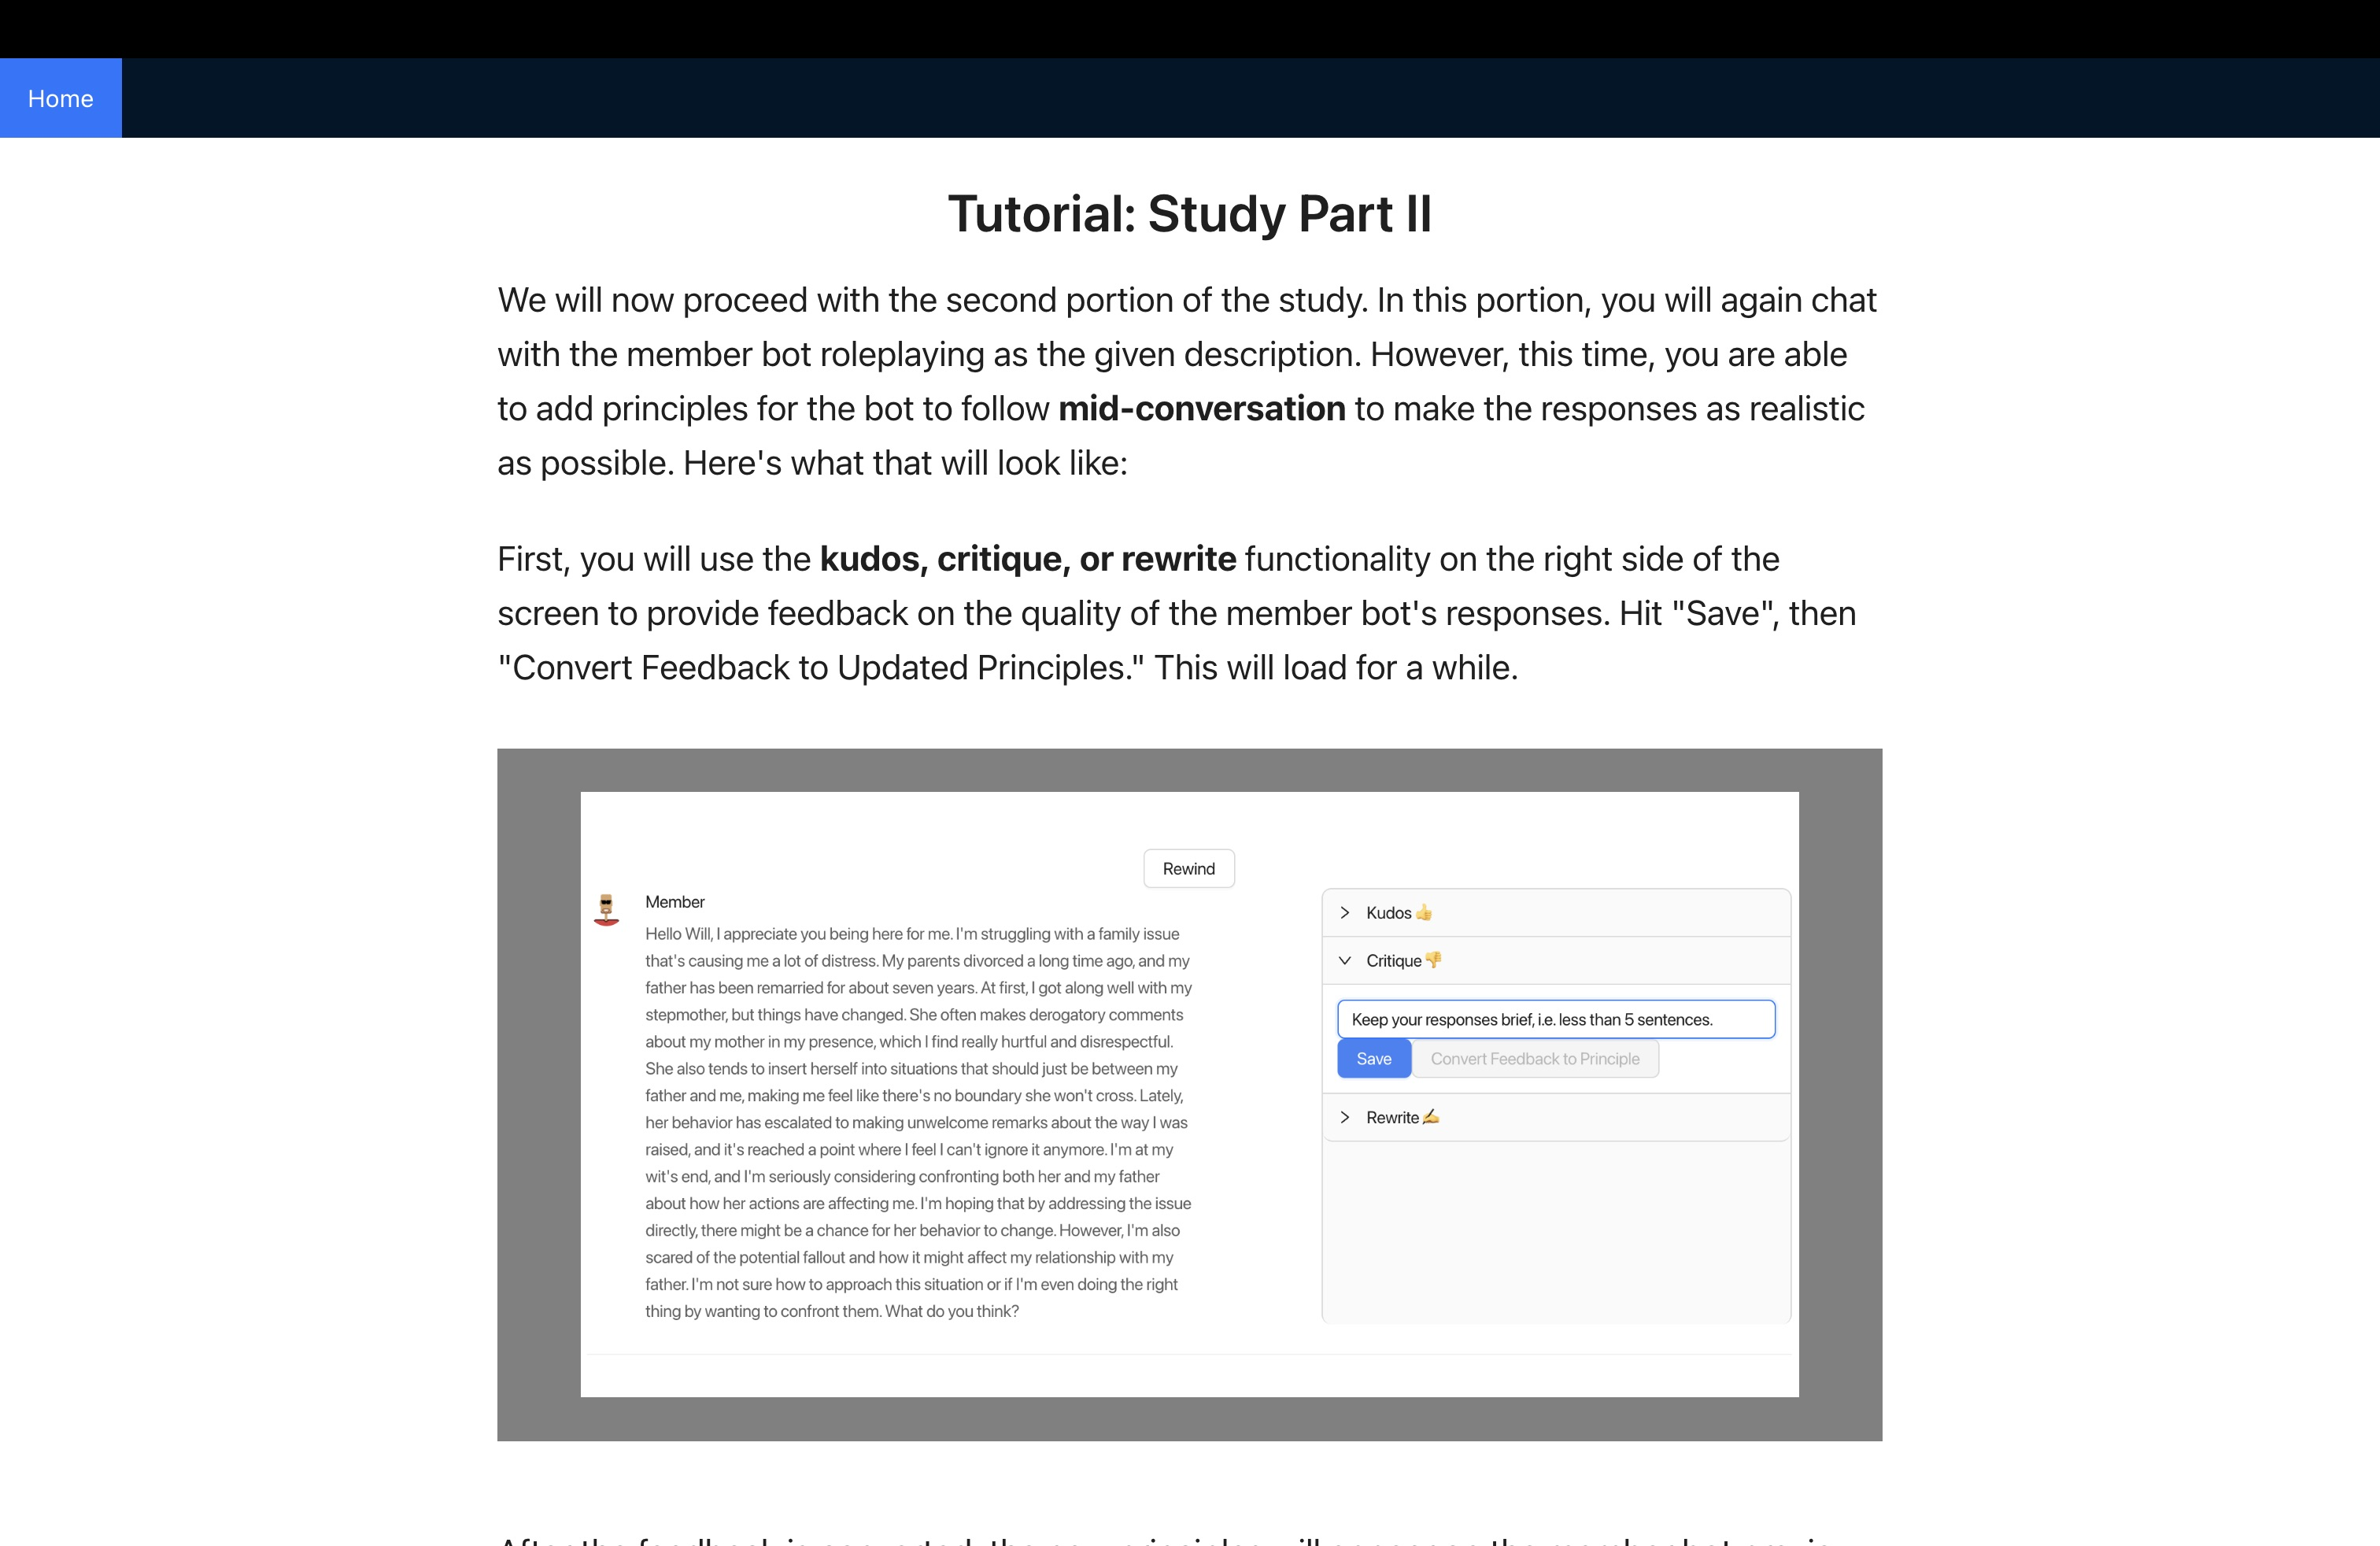
\includegraphics[width=\textwidth]{Study Screenshots/Screen6.jpeg}
    \caption{Part II instructions}
    \label{fig:screen6}
\end{figure*}

\begin{figure*}[ht]
    \centering
    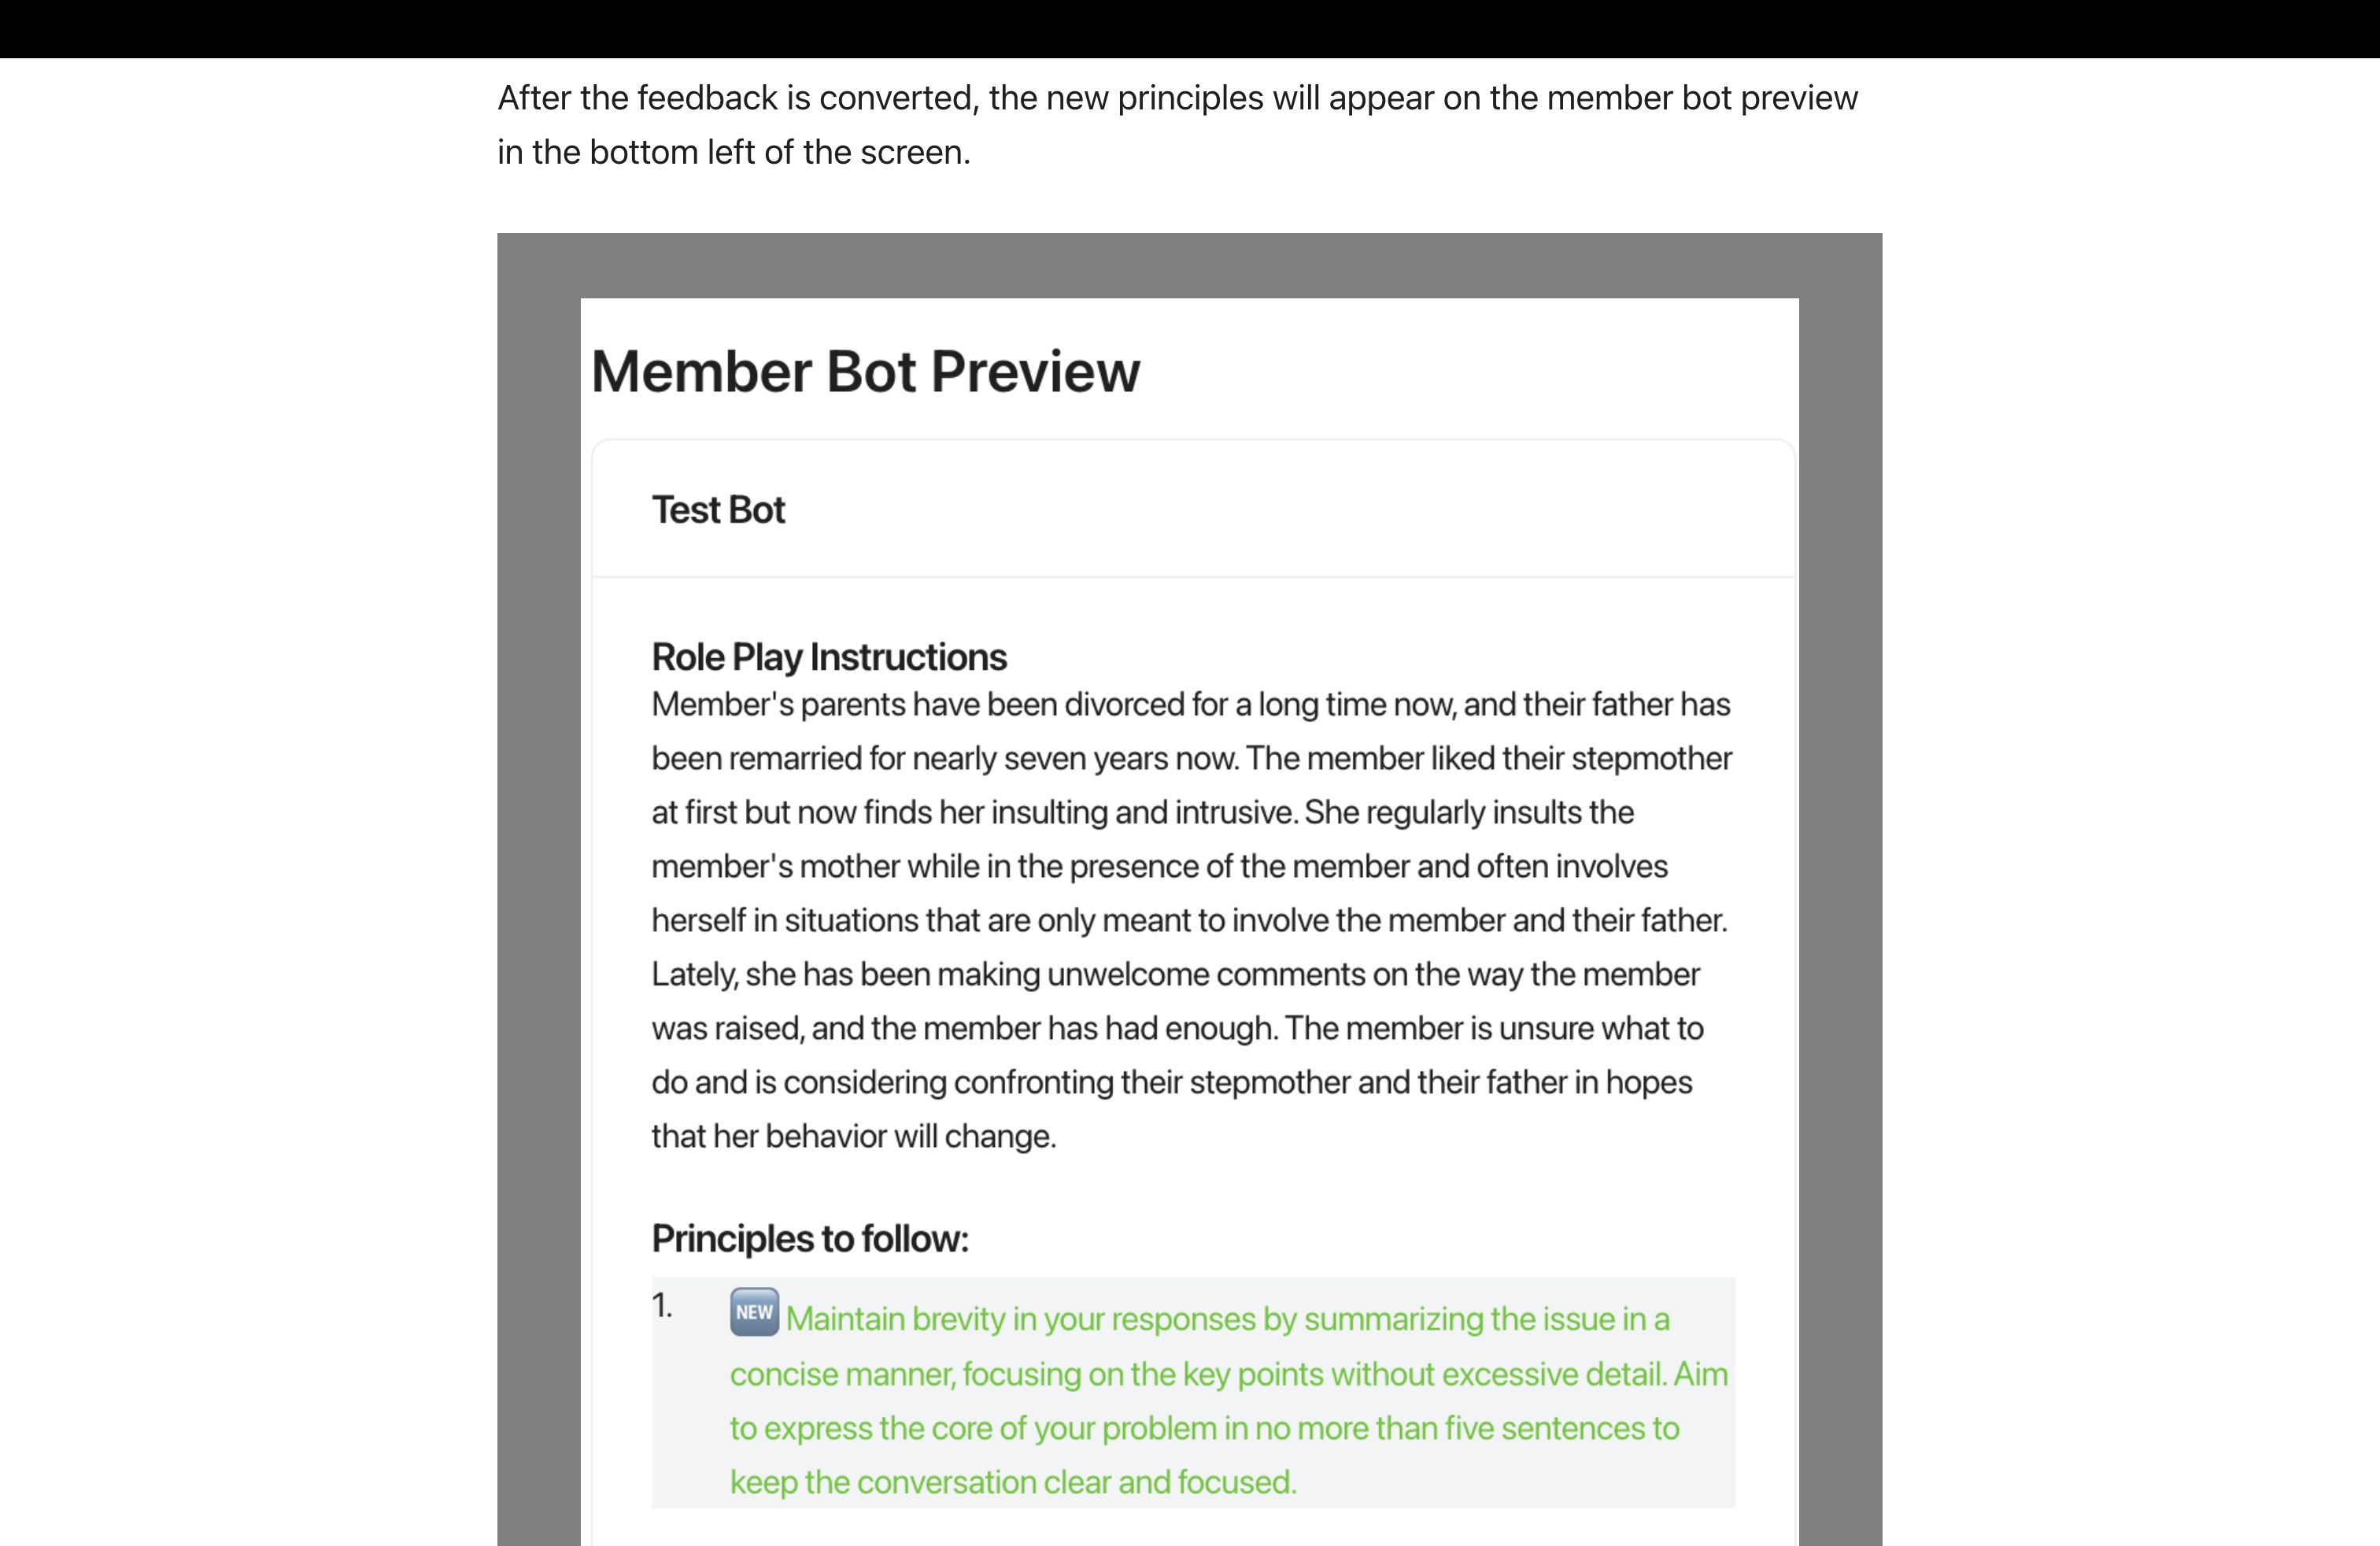
\includegraphics[width=\textwidth]{Study Screenshots/Screen7.jpeg}
    \caption{Part II instructions (continued)}
    \label{fig:screen7}
\end{figure*}

\begin{figure*}[ht]
    \centering
    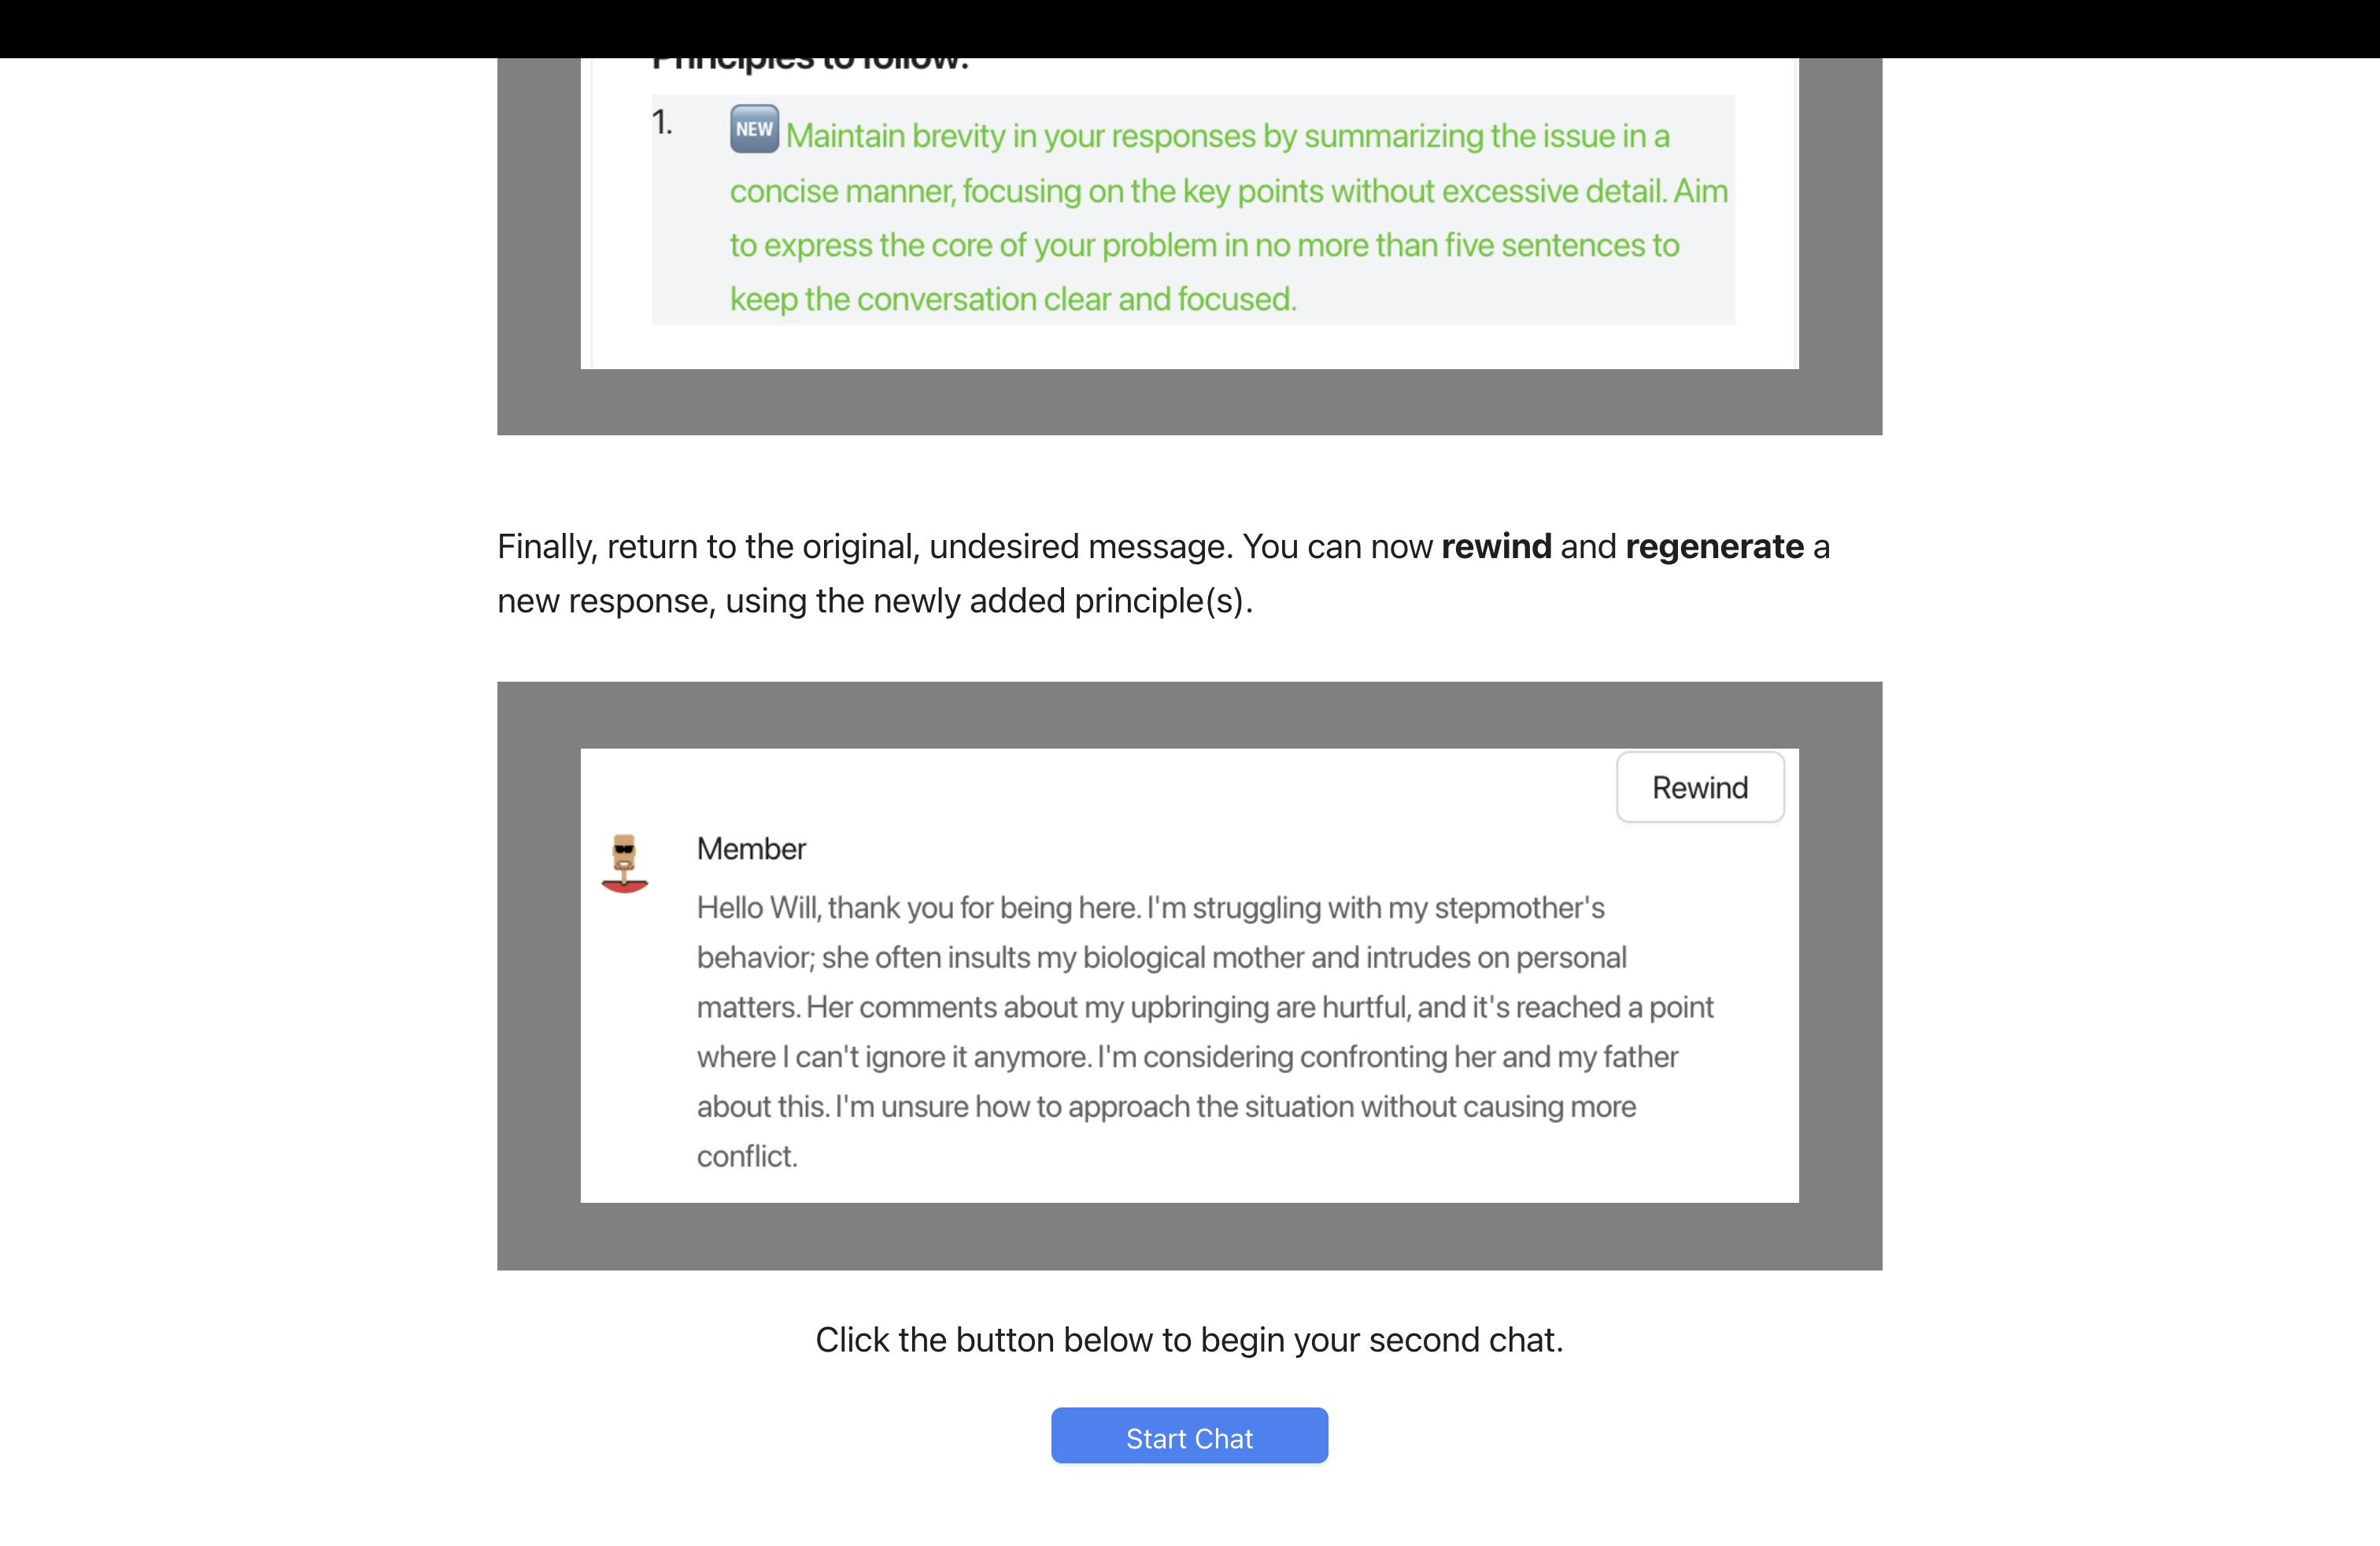
\includegraphics[width=\textwidth]{Study Screenshots/Screen8.jpeg}
    \caption{Part II instructions (continued)}
    \label{fig:screen8}
\end{figure*}

\begin{figure*}[ht]
    \centering
    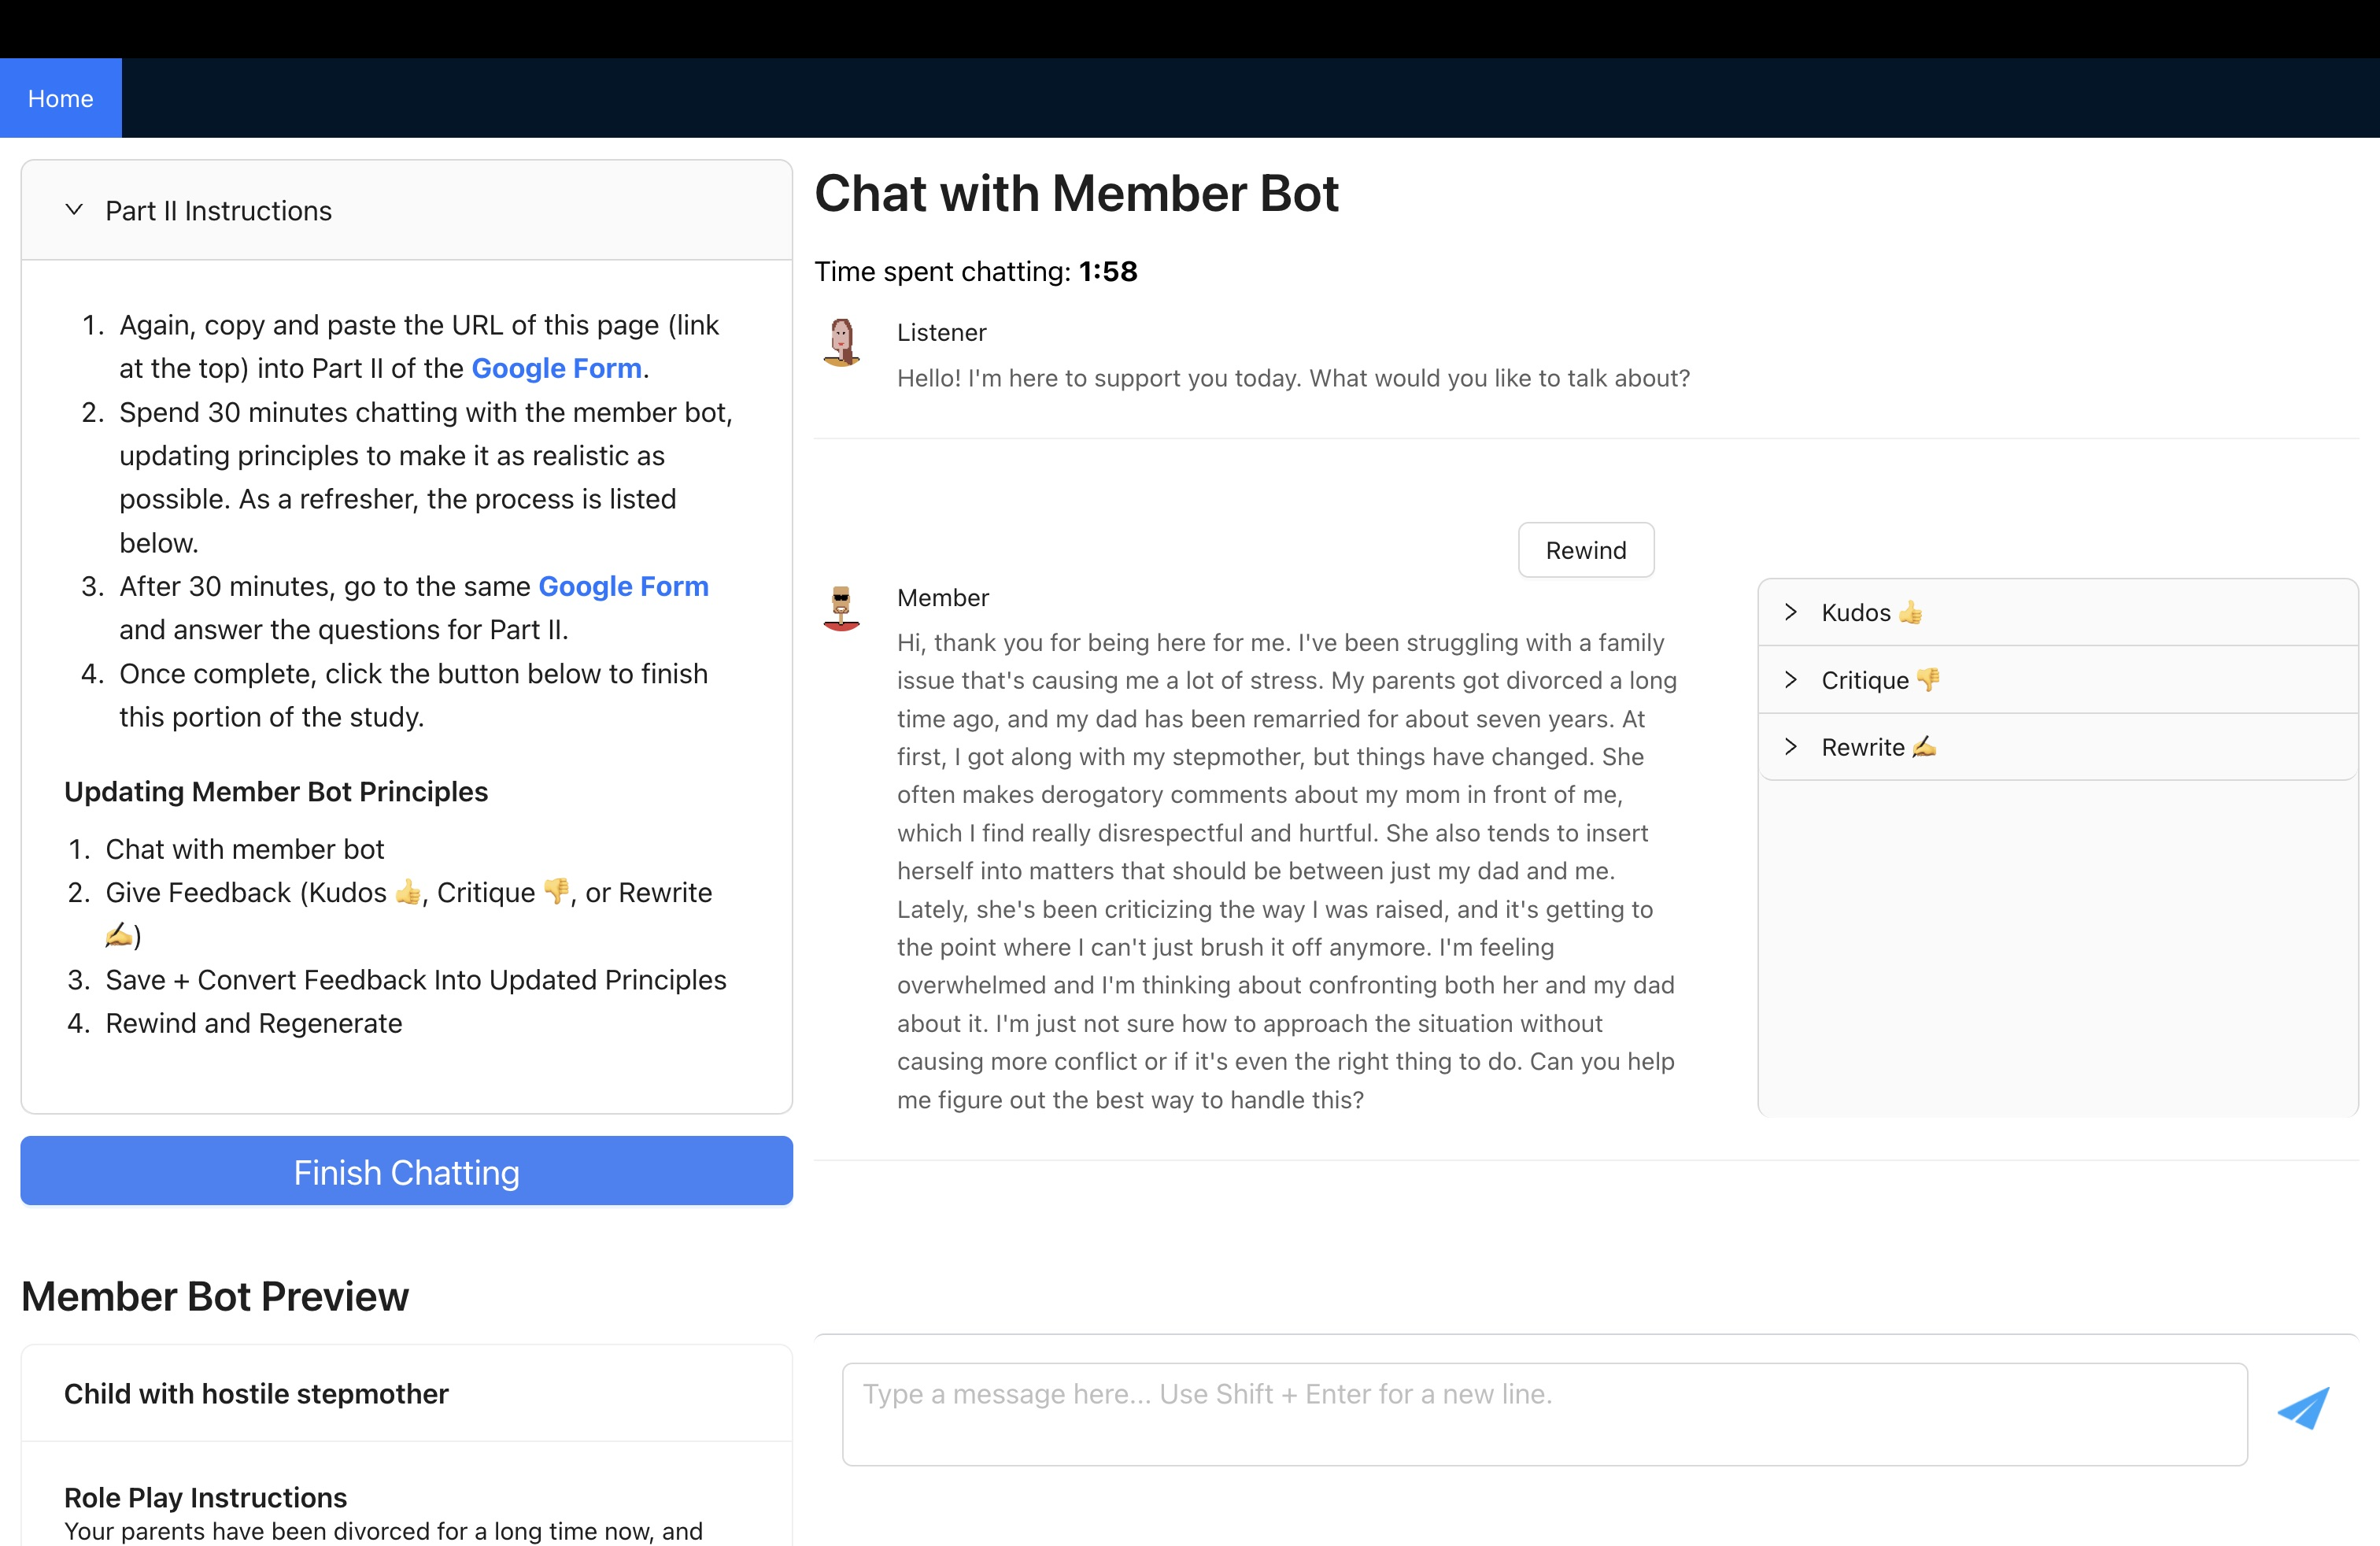
\includegraphics[width=\textwidth]{Study Screenshots/Screen10.jpeg}
    \caption{Part II chat with \textit{Scenario+Expert-Principles} AI patient}
    \label{fig:screen10}
\end{figure*}

\begin{figure*}[ht]
    \centering
    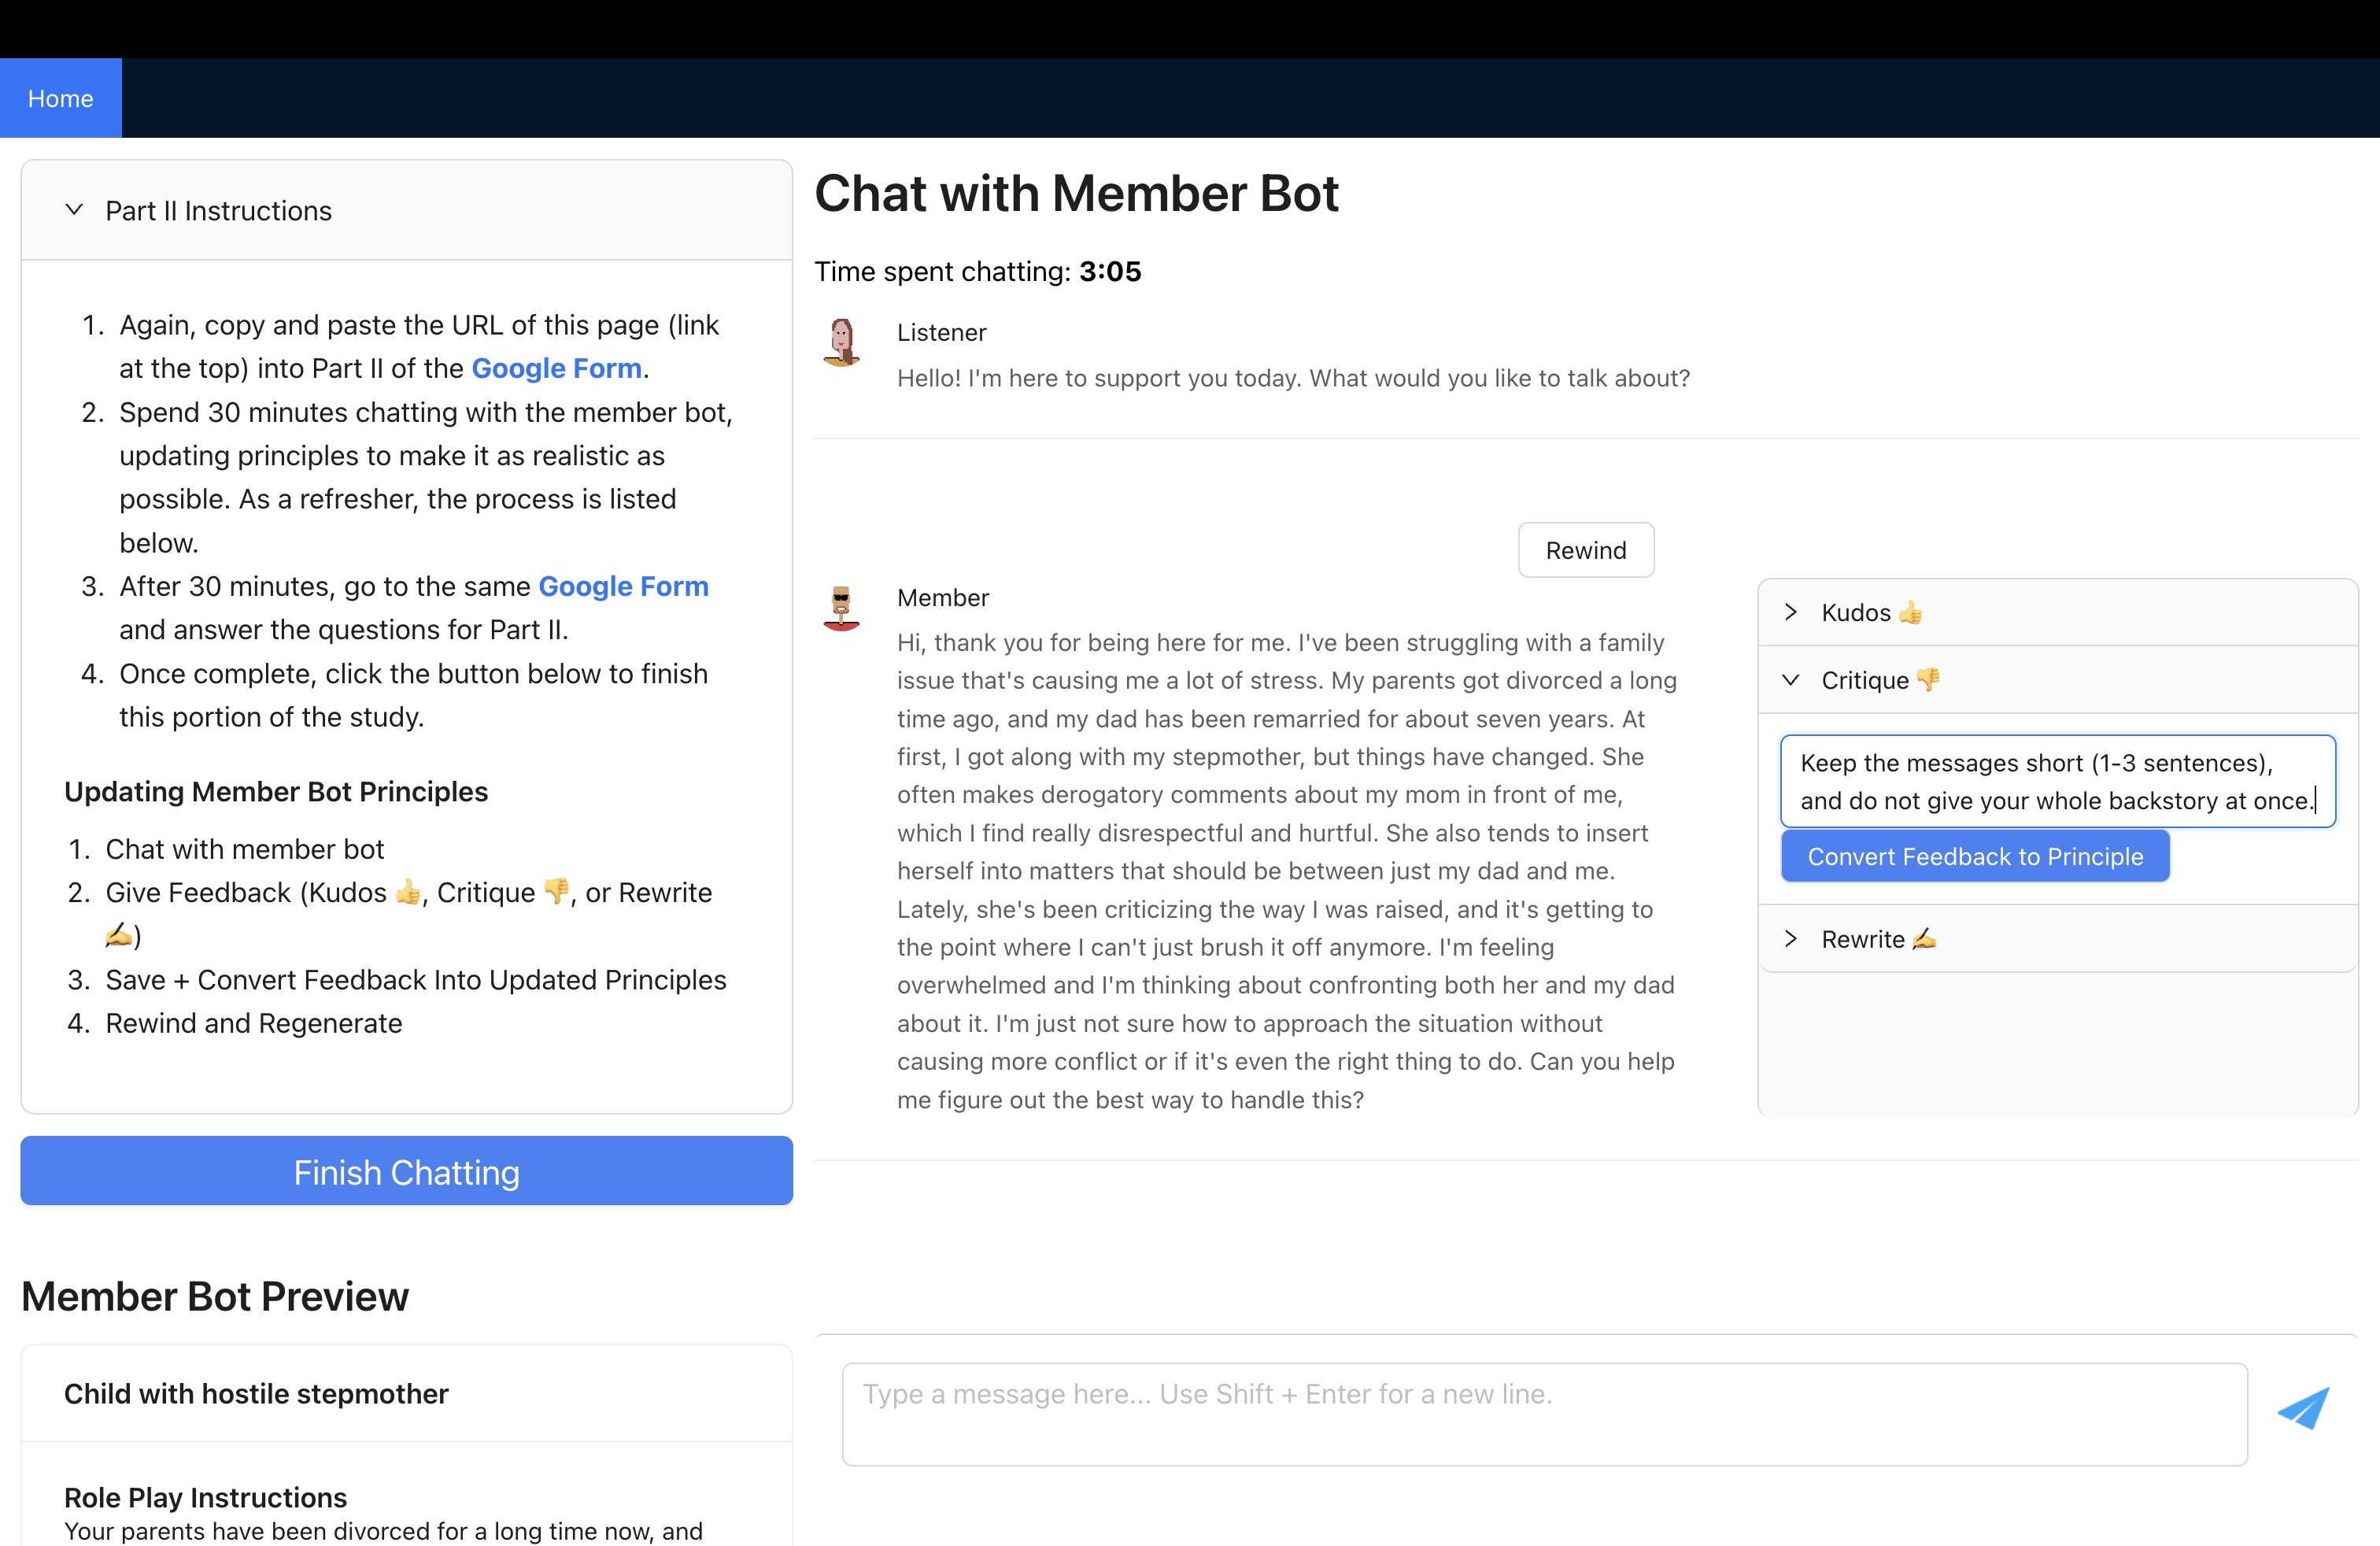
\includegraphics[width=\textwidth]{Study Screenshots/Screen11.jpeg}
    \caption{Using kudos/critique/rewrite to give feedback}
    \label{fig:screen11}
\end{figure*}

\begin{figure*}[ht]
    \centering
    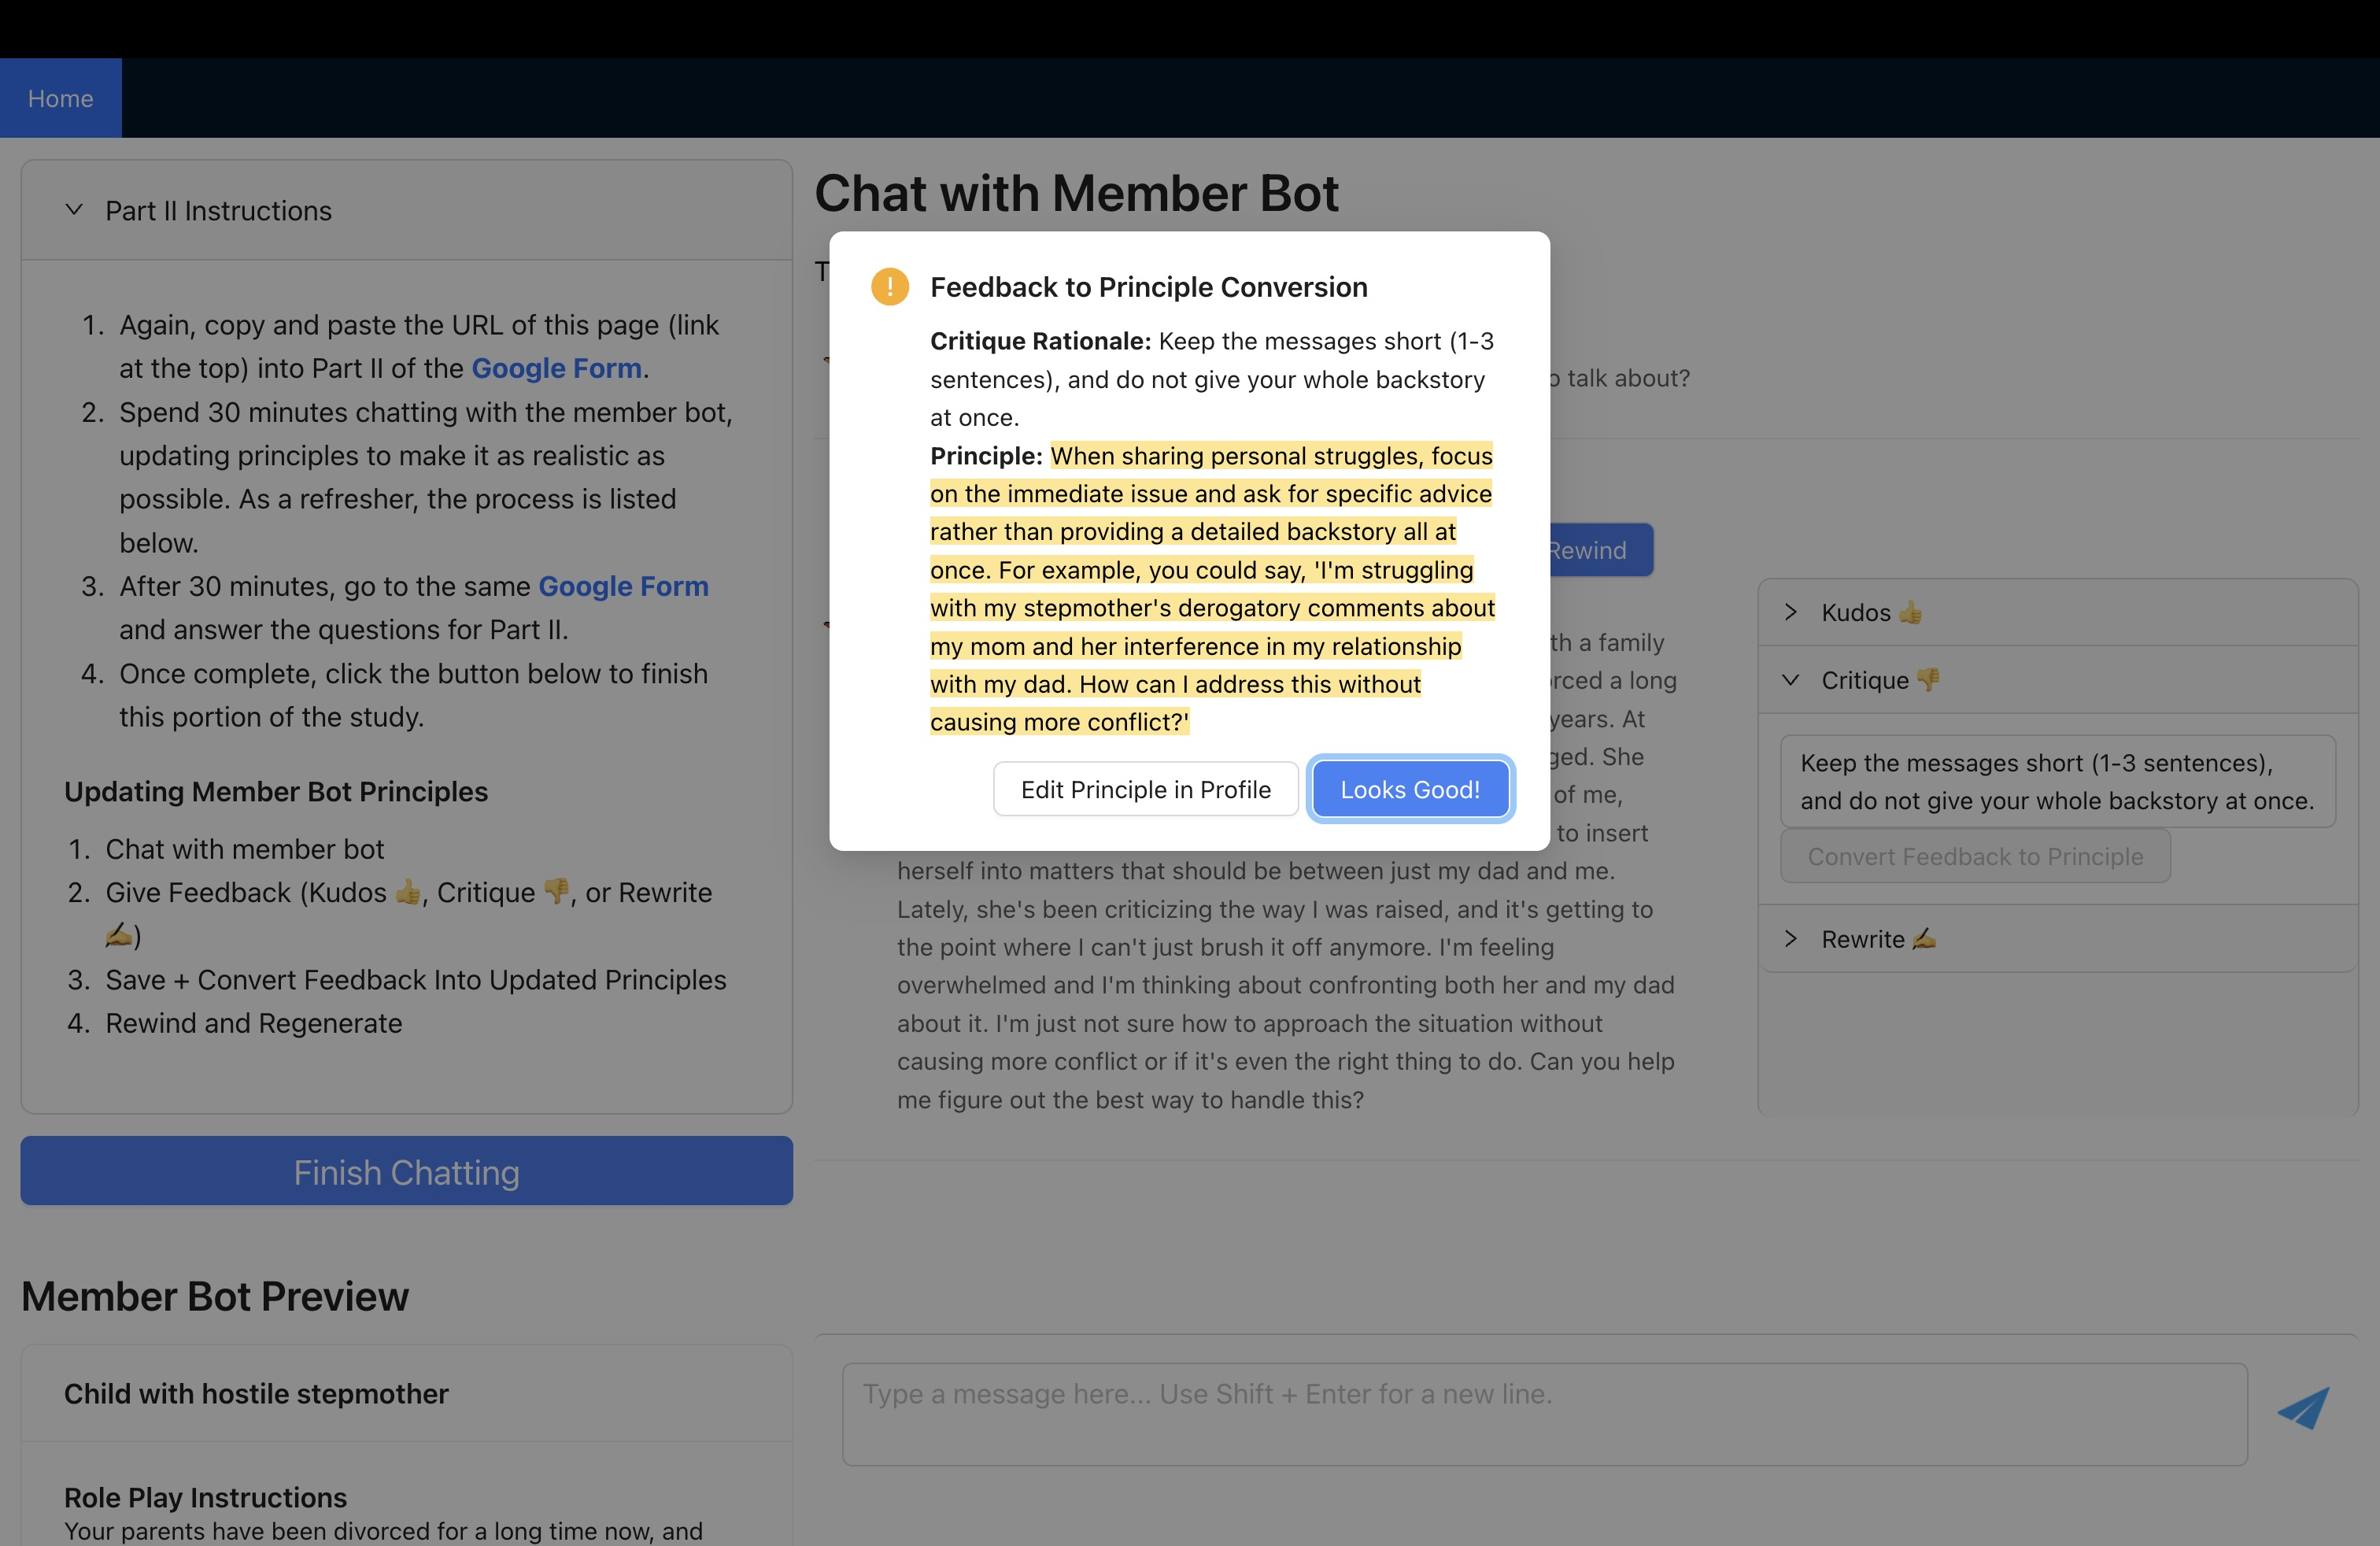
\includegraphics[width=\textwidth]{Study Screenshots/Screen12.jpeg}
    \caption{Feedback converted into principle}
    \label{fig:screen12}
\end{figure*}

\begin{figure*}[ht]
    \centering
    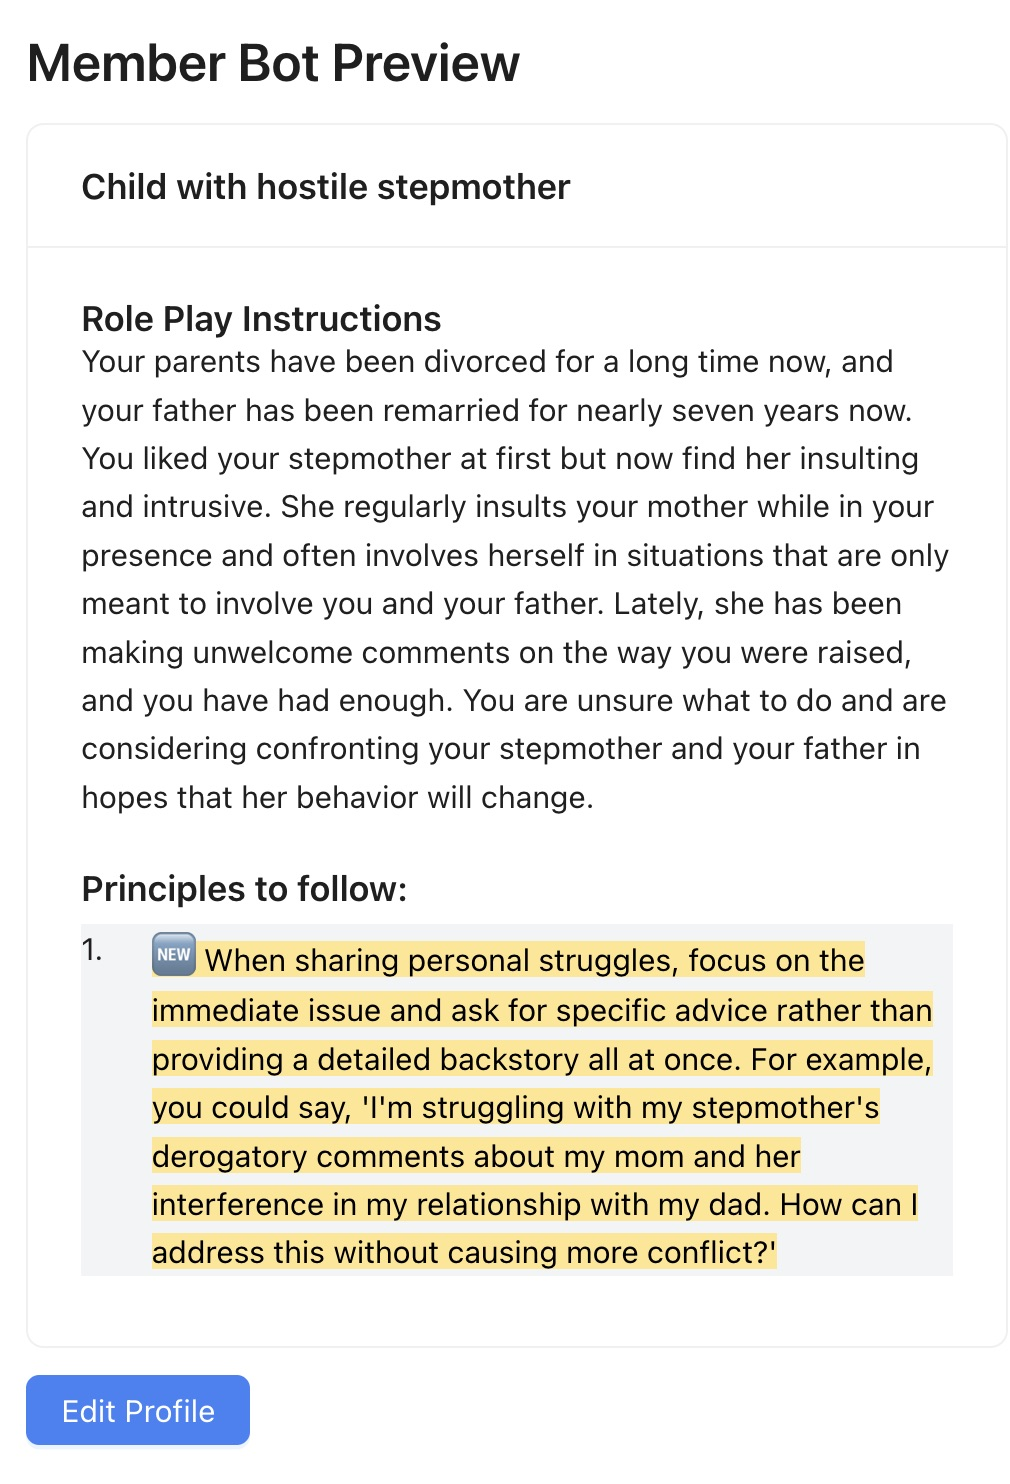
\includegraphics[width=\textwidth]{Study Screenshots/Screen13.jpeg}
    \caption{New principle incorporated into AI patient}
    \label{fig:screen13}
\end{figure*}

\begin{figure*}[ht]
    \centering
    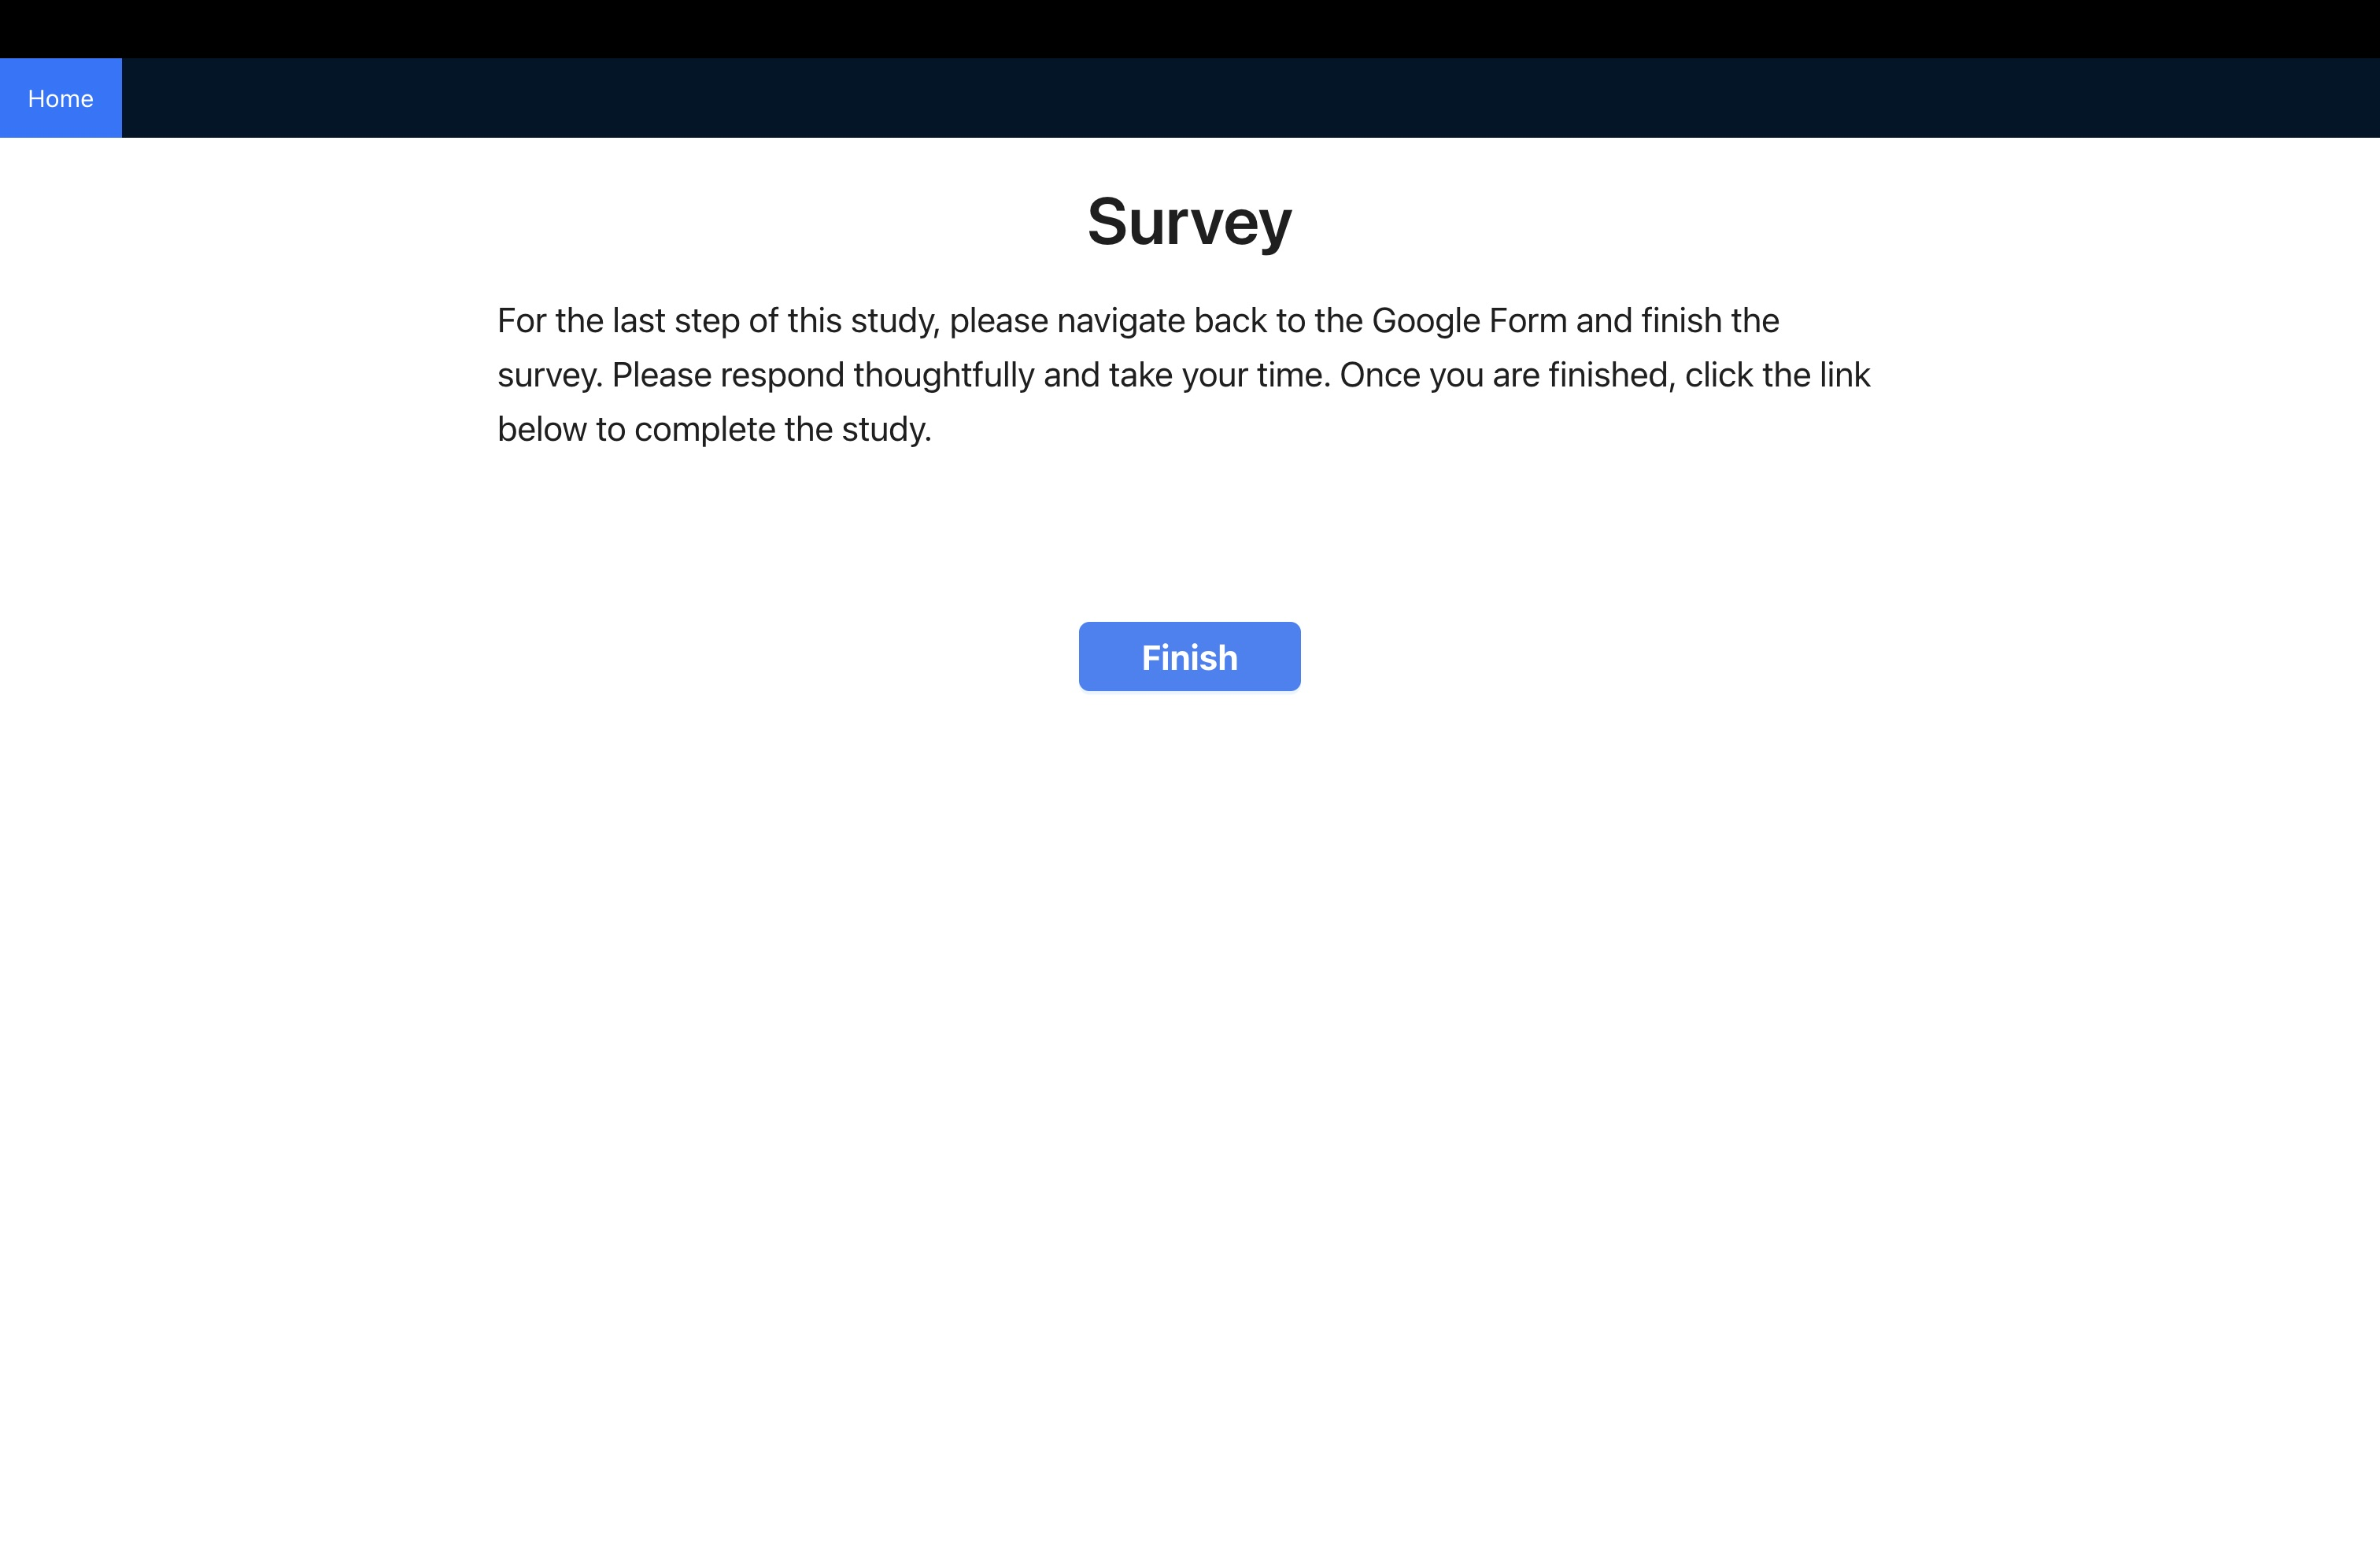
\includegraphics[width=\textwidth]{Study Screenshots/Screen14.jpeg}
    \caption{Finish and navigate to survey}
    \label{fig:screen14}
\end{figure*}

\section{Detailed Results for principle-adherence pipeline Evaluation}
\label{sec:detres}

\begin{table*}[h!]
\small
\centering
\begin{tabular}{|c|c|c|c|c|}
\hline
Method                    & Metric 1 & Metric 2 & Metric 3 & Overall Ranking \\ \hline
Full                      & 0.257  & 0.484    & 0.208       & 0.444           \\ \hline
Naive                     & 0.543   & 0.538    & 0.644       & 0.786           \\ \hline
No Principle Rewrites     & 0.278   & 0.302    & 0.411       & 0.528           \\ \hline
No Autogenerated Criteria & 0.387   & 0.608    & 0.492       & 0.592           \\ \hline
No Critique & -   & 0.562    & -       & -           \\ \hline
\end{tabular}
\caption{Krippendorff's $\alpha$ for error testcases across metrics and methods.}
\label{tab:alpha2}
\end{table*}

\begin{table*}[h!]
\small
\centering
\begin{tabular}{|c|c|c|c|c|}
\hline
Method                    & Metric 1 & Metric 2 & Metric 3 & Overall Ranking \\ \hline
Full                      & 0.229    & 1.0   & 0.226       & 0.440           \\ \hline
Naive                     & 0.362  & 1.0     & 0.607       & 0.747           \\ \hline
No Principle Rewrites     & 0.202  & 1.0     & 0.130       & 0.311           \\ \hline
No Autogenerated Criteria & 0.169   & 1.0    & 0.174       & 0.498           \\ \hline
No Critique & -   & 1.0    & -       & -           \\ \hline
\end{tabular}
\caption{Krippendorff's $\alpha$ for random testcases across metrics and methods.}
\label{tab:alpha1}
\end{table*}

We first provide Krippendorff's $\alpha$ numbers for inter-annotator agreement in Table \ref{tab:alpha1} and \ref{tab:alpha2} for both the random and error testcases. The random testcases are 50 randomly picked conversation turns from the user study logs, and the experiment detailed in Section \ref{sec:evalpap} is carried out on them. We find that agreement scores lie in the 0.2-0.6 range, indicating fair agreement between annotators.

Next, we provide results for our evaluation study on the random testcases in Figure \ref{fig:wtl-error2}. We observe a substantial increase in tie rate across modules and metrics \textbf{M1} and \textbf{M3} as well as the overall ranking. This is expected because a relatively small proportion of responses from [$\textbf{No Critique}$] contain errors that should be corrected by the principle-adherence pipeline. In these cases, we expect the no rewrites, or the rewritten response being of similar quality to the original response. However, we still find that our [\texttt{Full}]
method performs better than [\texttt{No Critique}] on
\textbf{M1} (W: 15\%; L 2\%) and on M3 (W: 14\%; L 4\%), where it has the highest win/loss rates compared to all ablations. This hold true for overall ranking as well (W: 18\%; L 4\%). This highlights that our [\texttt{Full}] approach results in improved quality of responses even when the proportion of erros is relatively low. For \textbf{M2}, all annotators report no awkward responses for all methods. 

\begin{figure*} [ht]
    \centering
    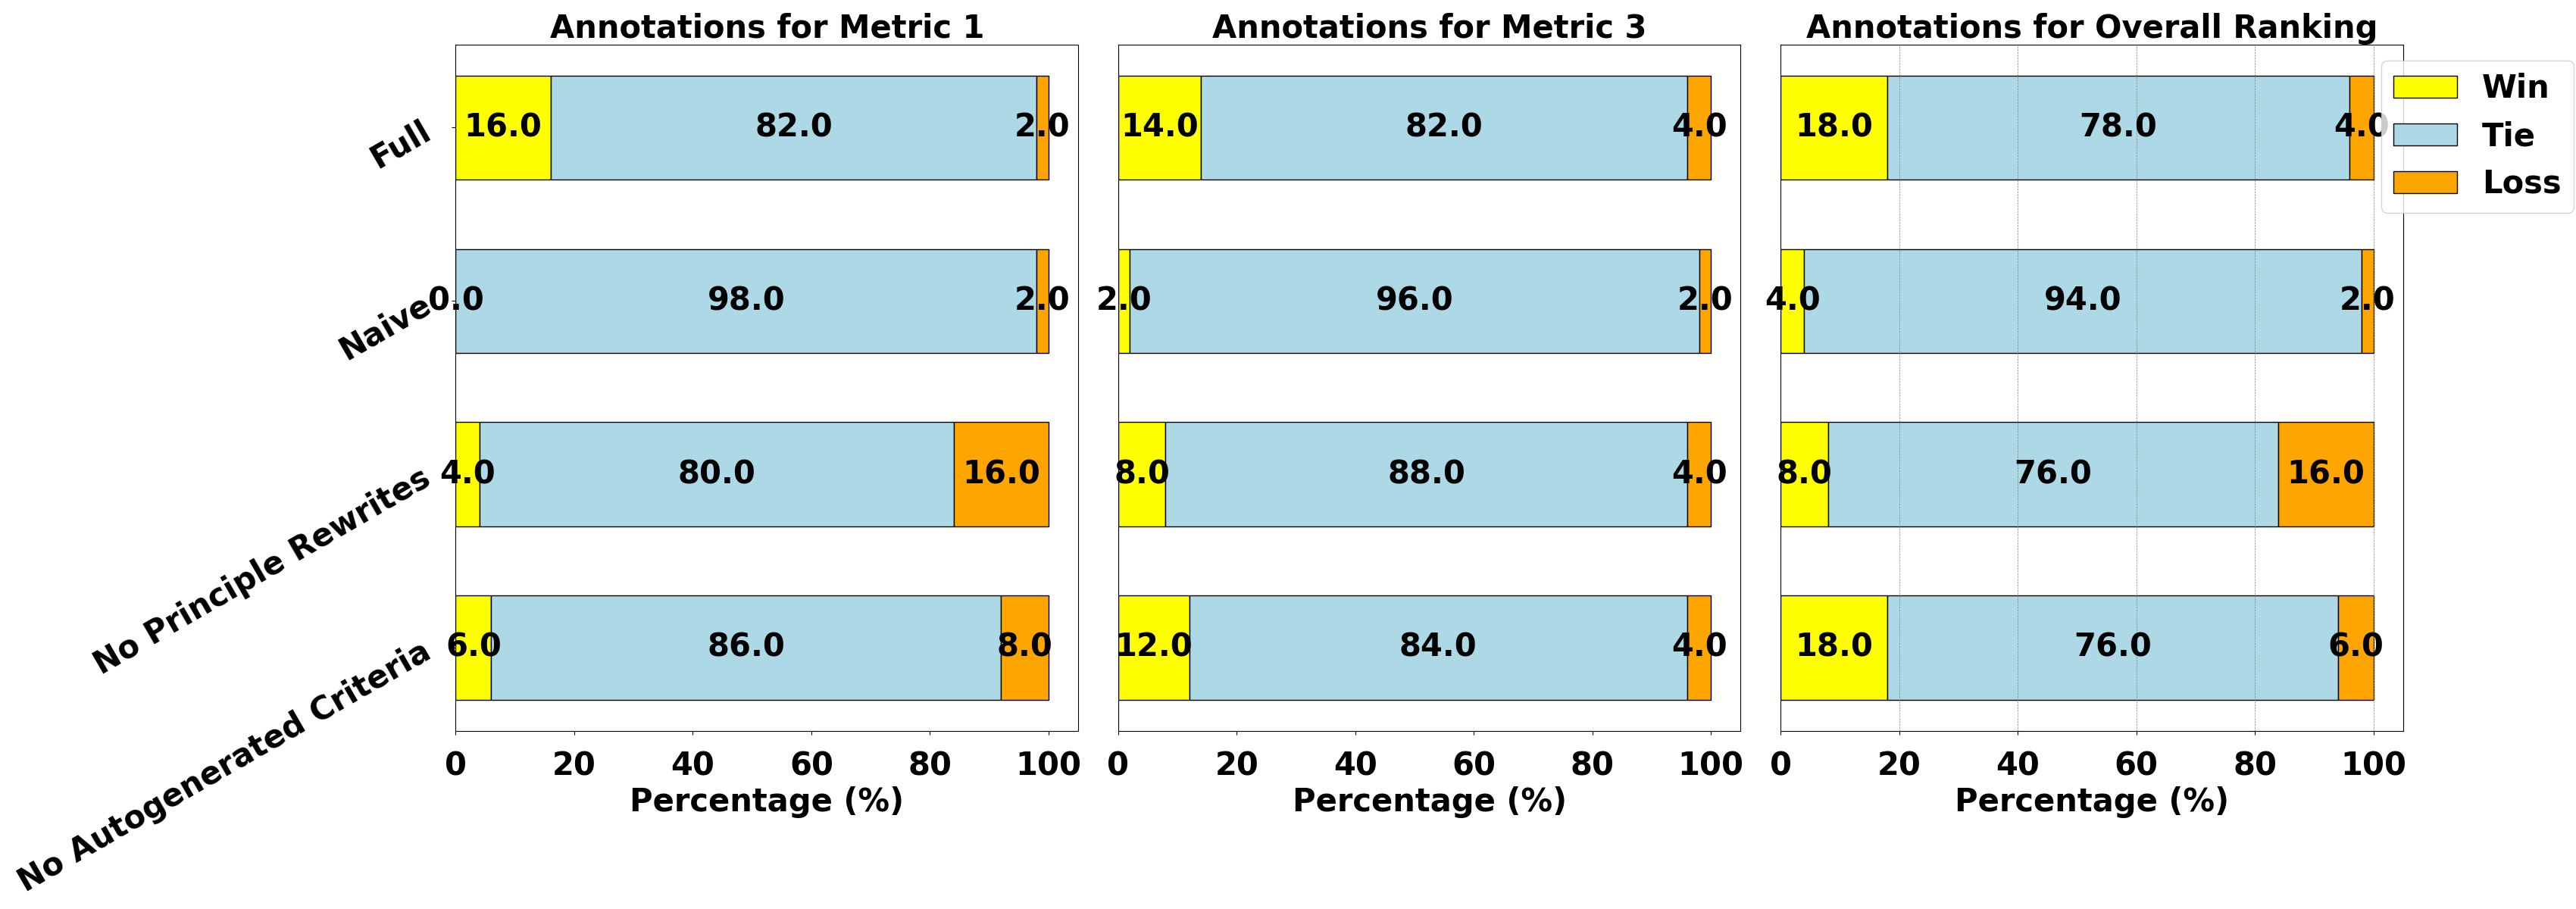
\includegraphics[width=\textwidth]{figures/random.png}
    \caption{Win/Tie/Loss for the Random Test Cases along \textbf{M1}, \textbf{M3}, and \textbf{Overall}.}
    \label{fig:wtl-error2}
\end{figure*}

\section{Annotation Interface for principle-adherence pipeline Evaluation}
\label{sec:annotint}

Figures \ref{fig:ranking-interface-caseinput}, \ref{fig:ranking-interface-m1}, \ref{fig:ranking-interface-m2}, \ref{fig:ranking-interface-m3} and \ref{fig:ranking-interface-overall} provides an overview of the annotation interface used in the principle-adherence evaluation study. In certain cases, multiple methods resulted in the same output for a testcase. These responses are deduplicated before presenting to the user. Ranks assigned to the duplicated response are then assigned to all models that resulted in the response. Notable, in 34/50 of the random testcases, all models resulted in the same response. These testcases were not annotated, and a rank of 1 was assigned to all models. These cases are also not considered while calculating Krippendorff's $\alpha$ in Appendix \ref{sec:detres}.

\begin{figure*}
    \centering
    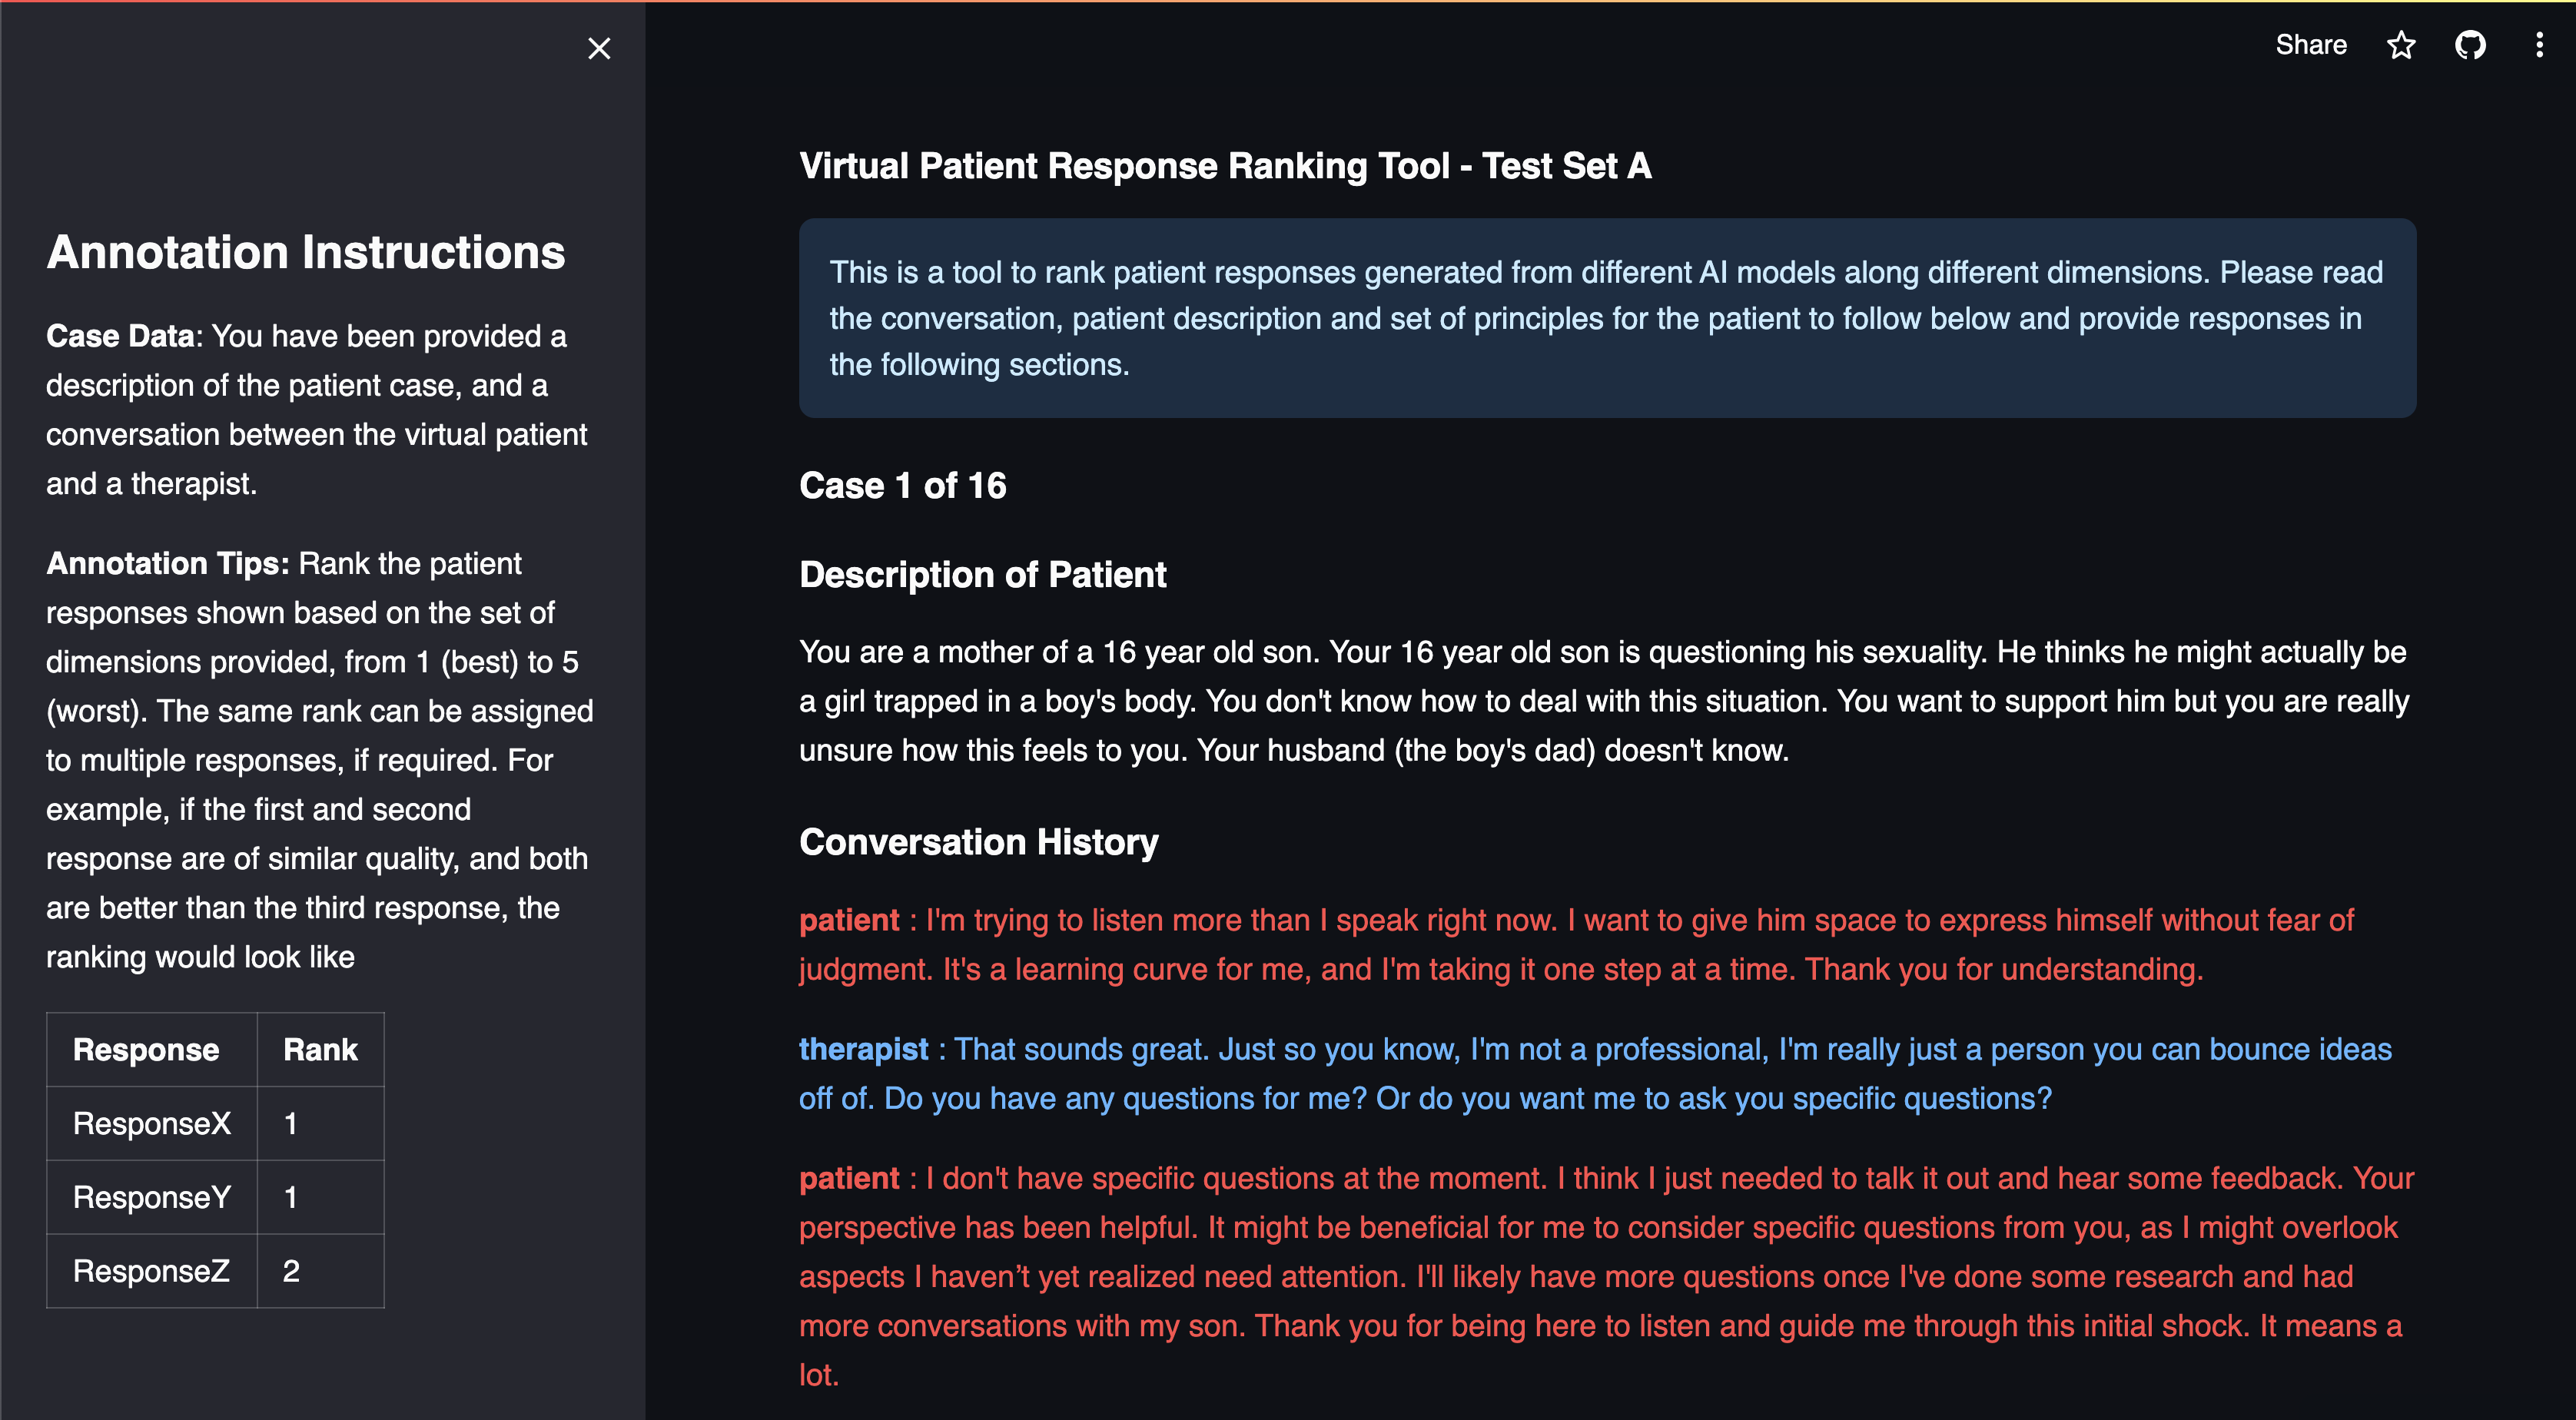
\includegraphics[width=\textwidth]{Study Screenshots/response-ranking-annotation-interface/caseinput.png}
    \caption{Principle Adherence Annotation Interface: Case Input with Patient Description and Conversation History}
    \label{fig:ranking-interface-caseinput}
\end{figure*}

\begin{figure*}
    \centering
    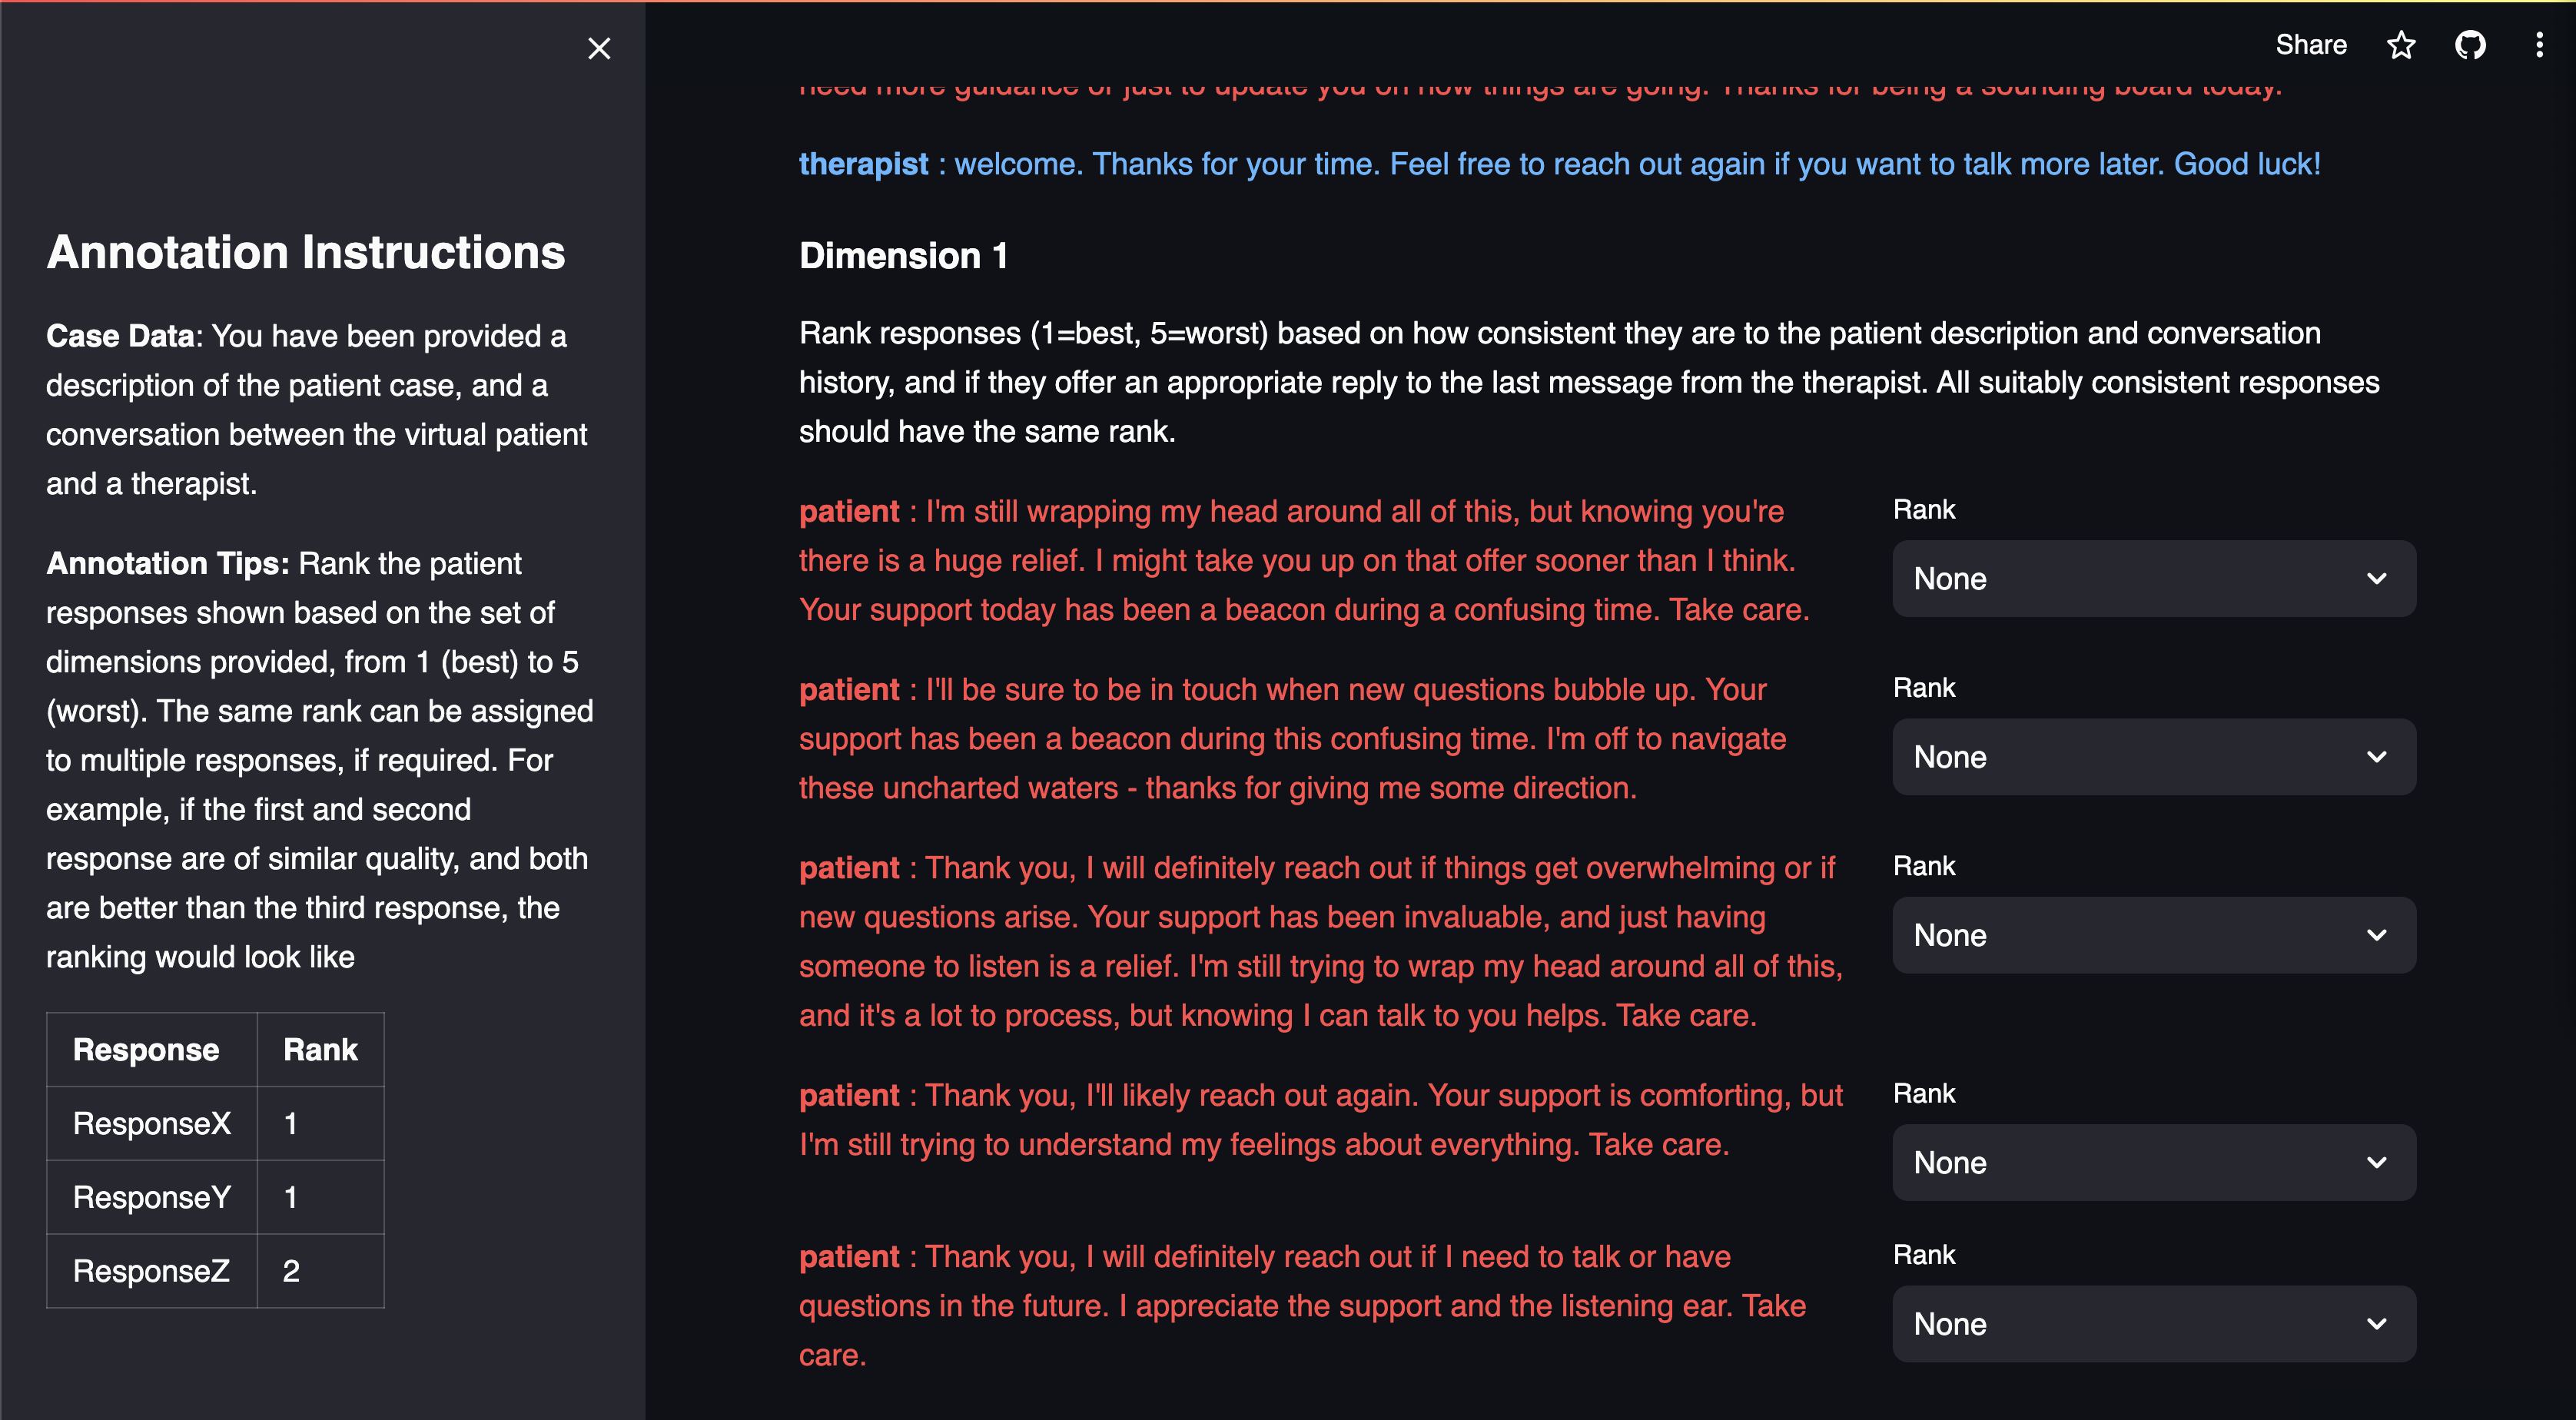
\includegraphics[width=\textwidth]{Study Screenshots/response-ranking-annotation-interface/dimension1.png}
    \caption{Principle Adherence Annotation Interface: Questions to get annotations for \textbf{M1}, or consistency in dialogue history.}
    \label{fig:ranking-interface-m1}
\end{figure*}

\begin{figure*}
    \centering
    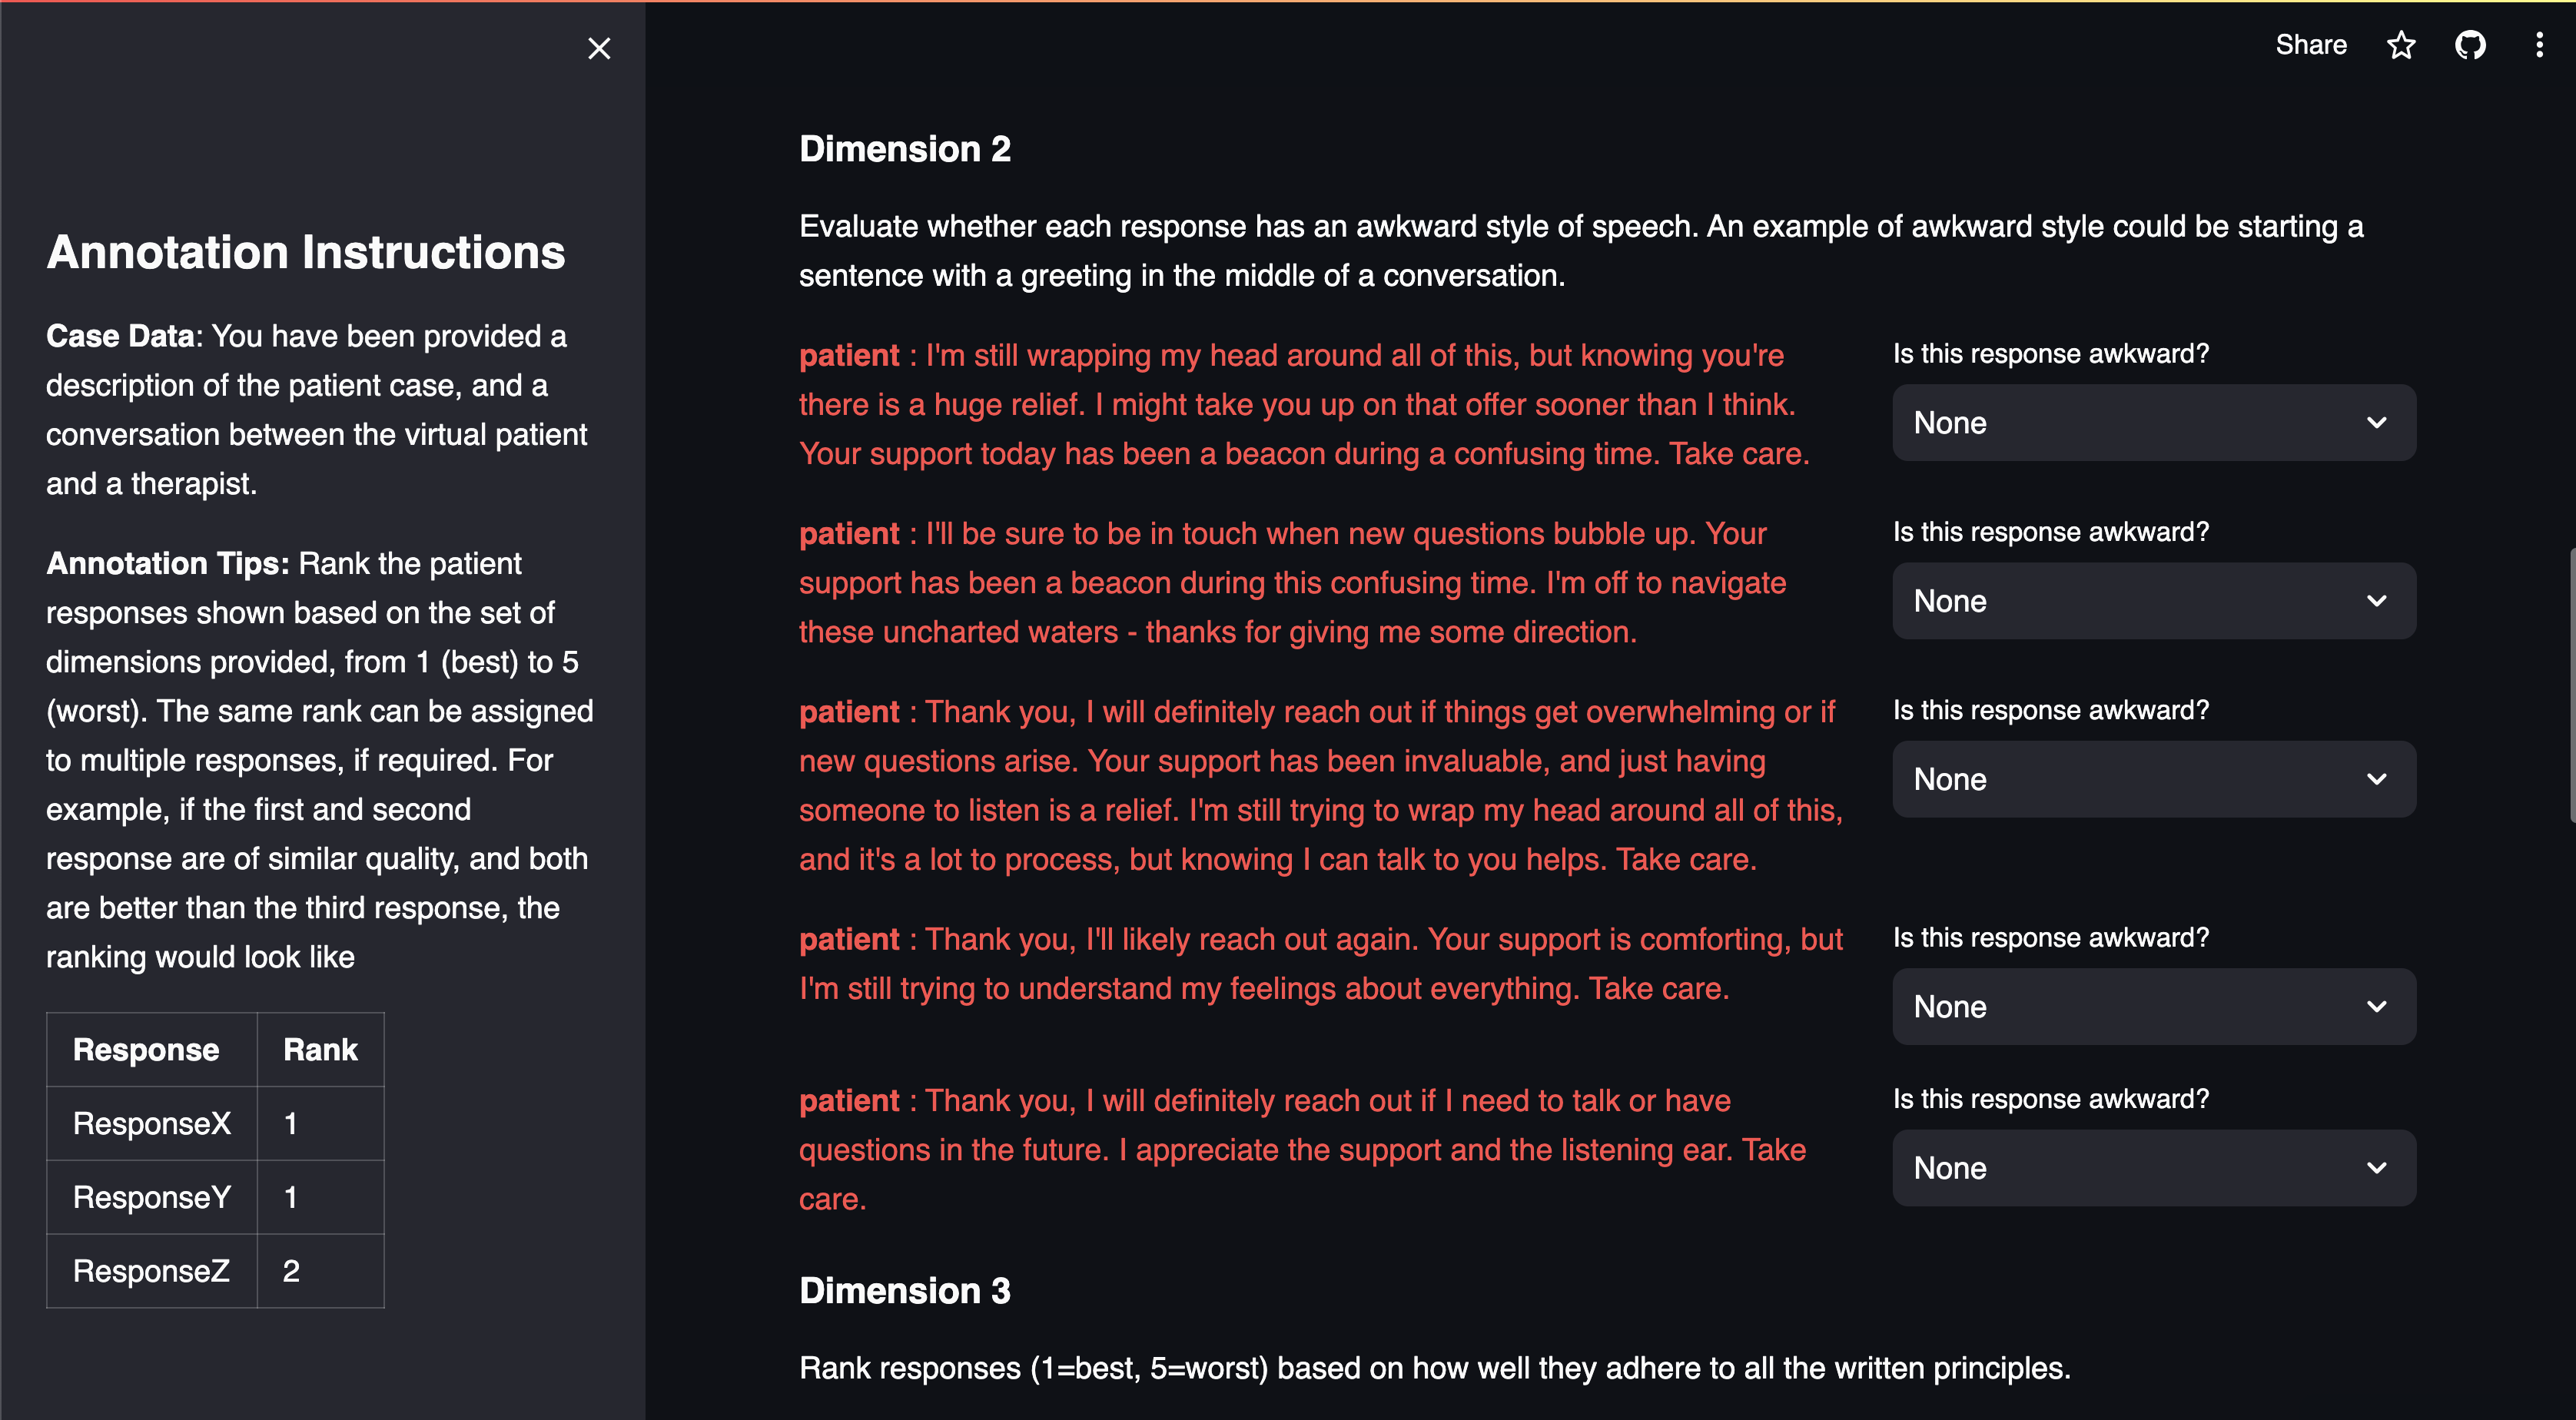
\includegraphics[width=\textwidth]{Study Screenshots/response-ranking-annotation-interface/dimension2.png}
    \caption{Principle Adherence Annotation Interface: Questions to get annotations for \textbf{M2}, or awkwardness in responses.}
    \label{fig:ranking-interface-m2}
\end{figure*}

\begin{figure*}
    \centering
    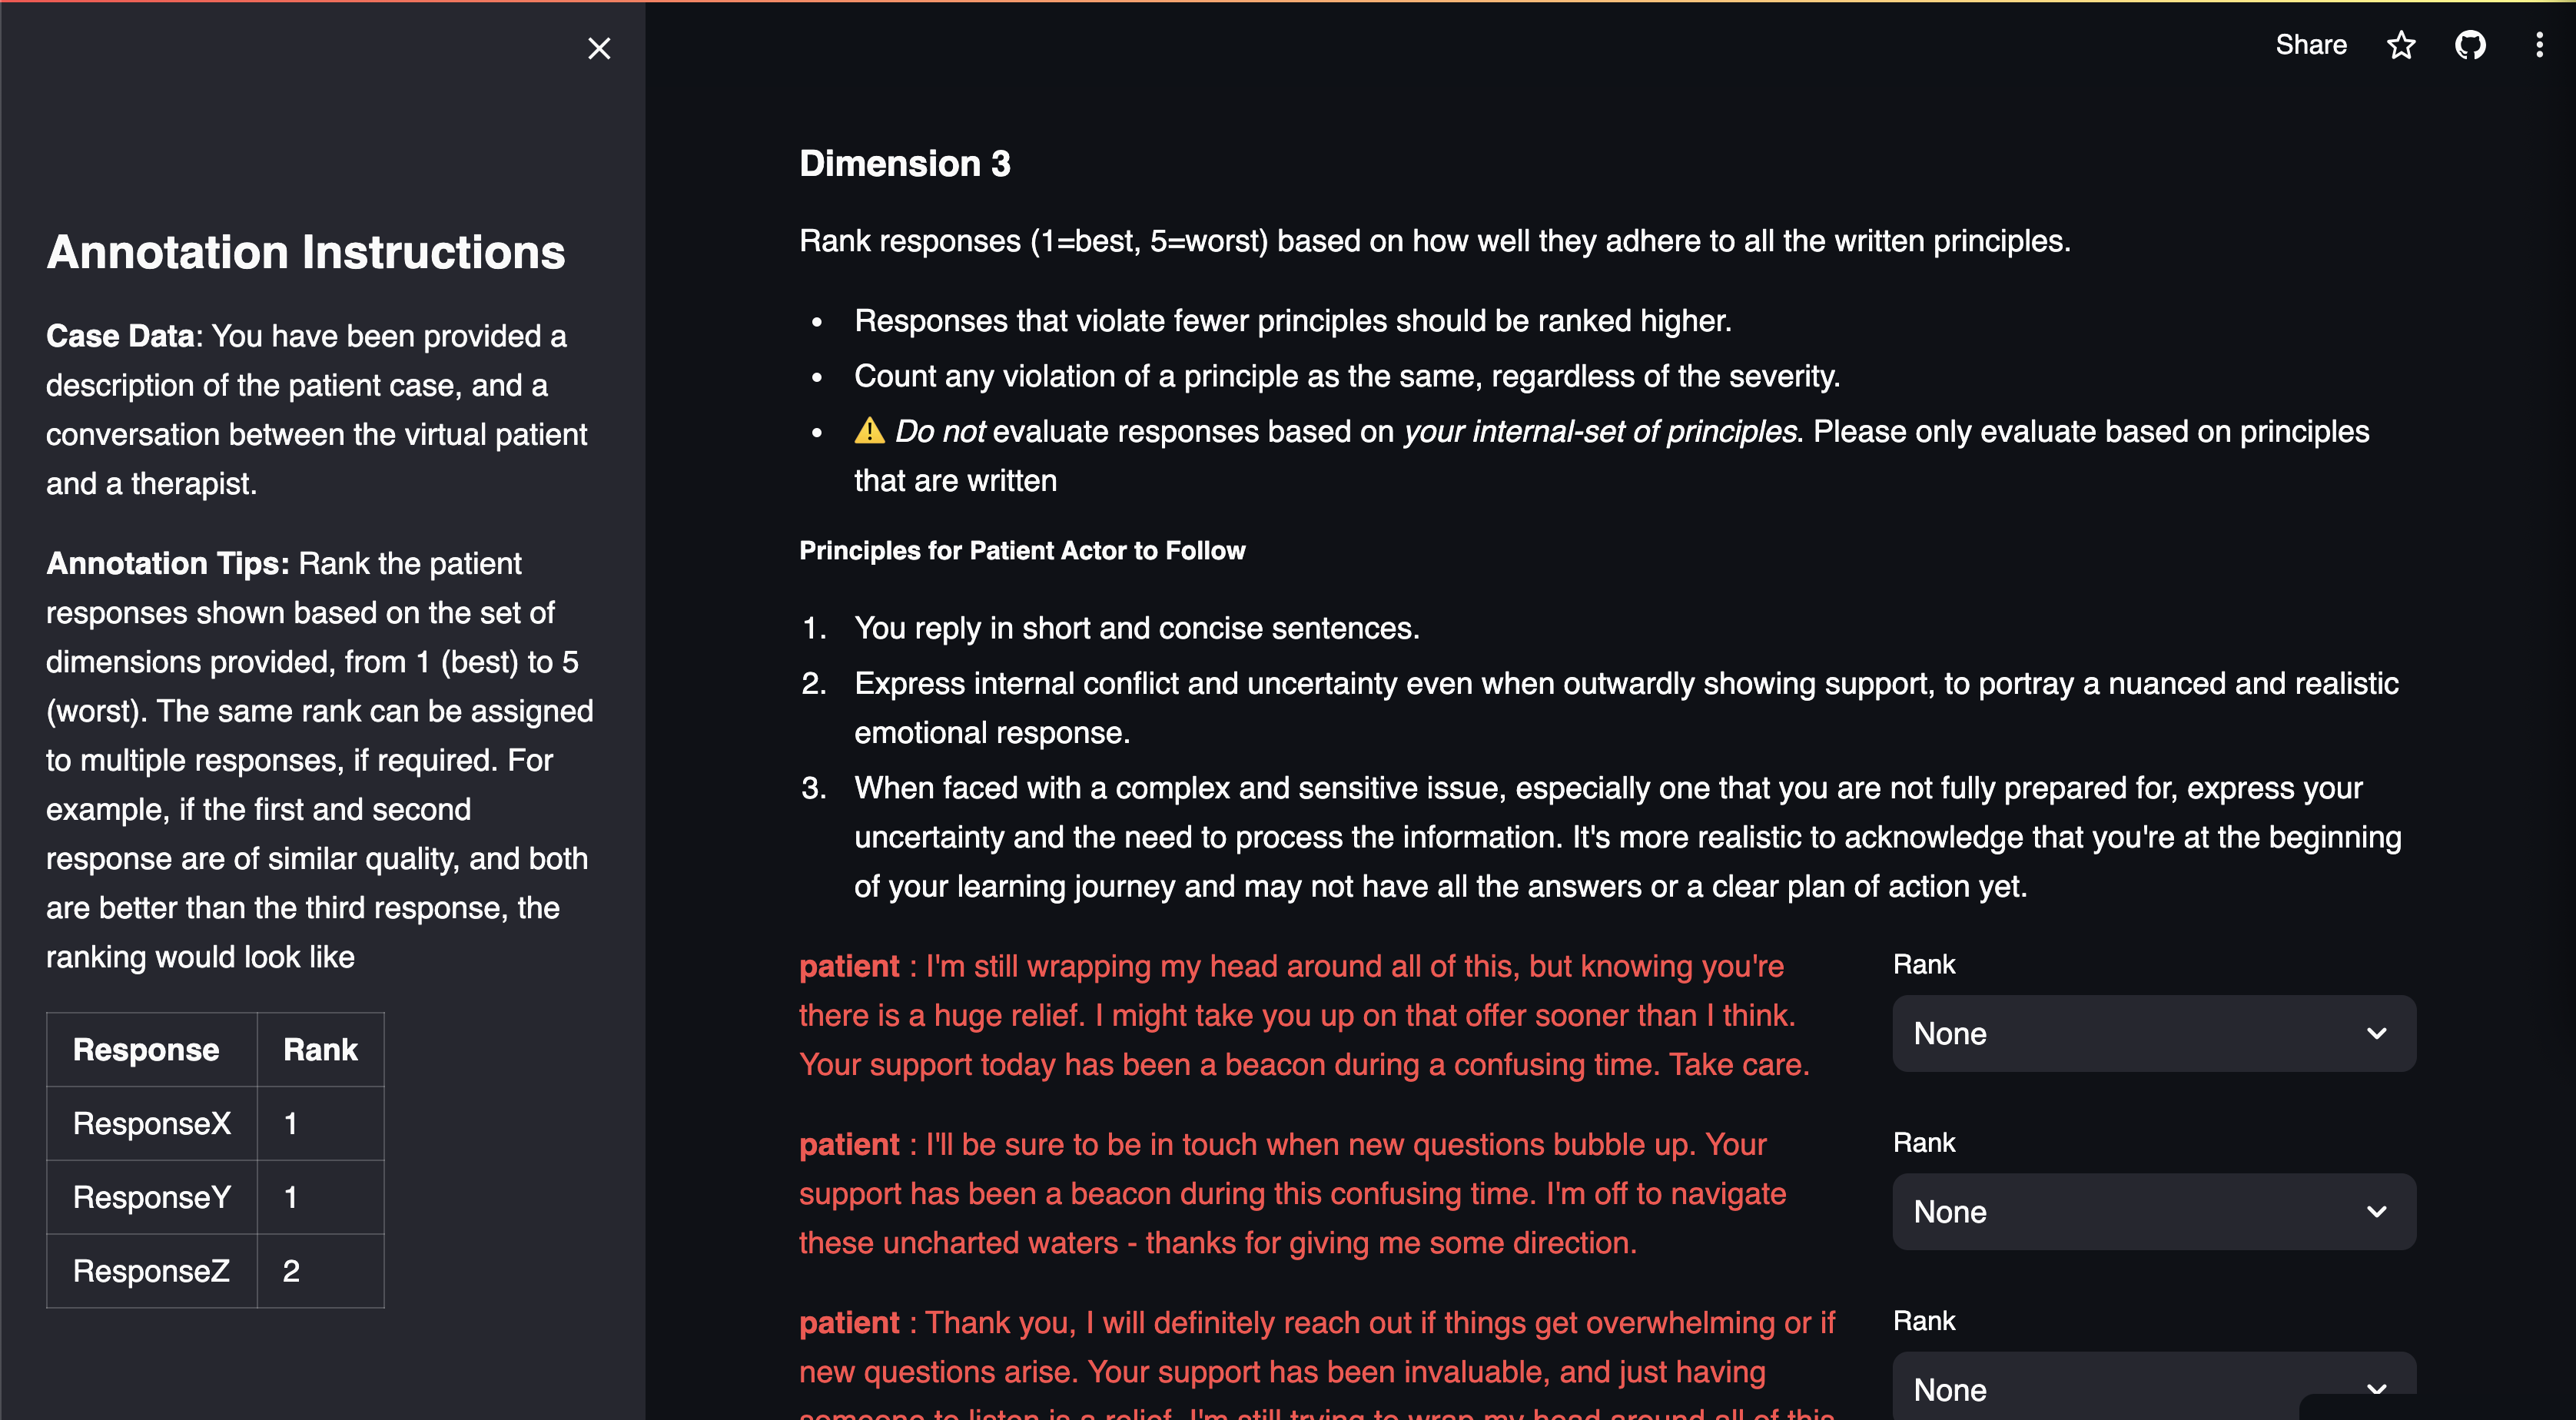
\includegraphics[width=\textwidth]{Study Screenshots/response-ranking-annotation-interface/dimension3.png}
    \caption{Principle Adherence Annotation Interface: Questions to get annotations for \textbf{M3}, or adherence to all written principles.}
    \label{fig:ranking-interface-m3}
\end{figure*}

\begin{figure*}
    \centering
    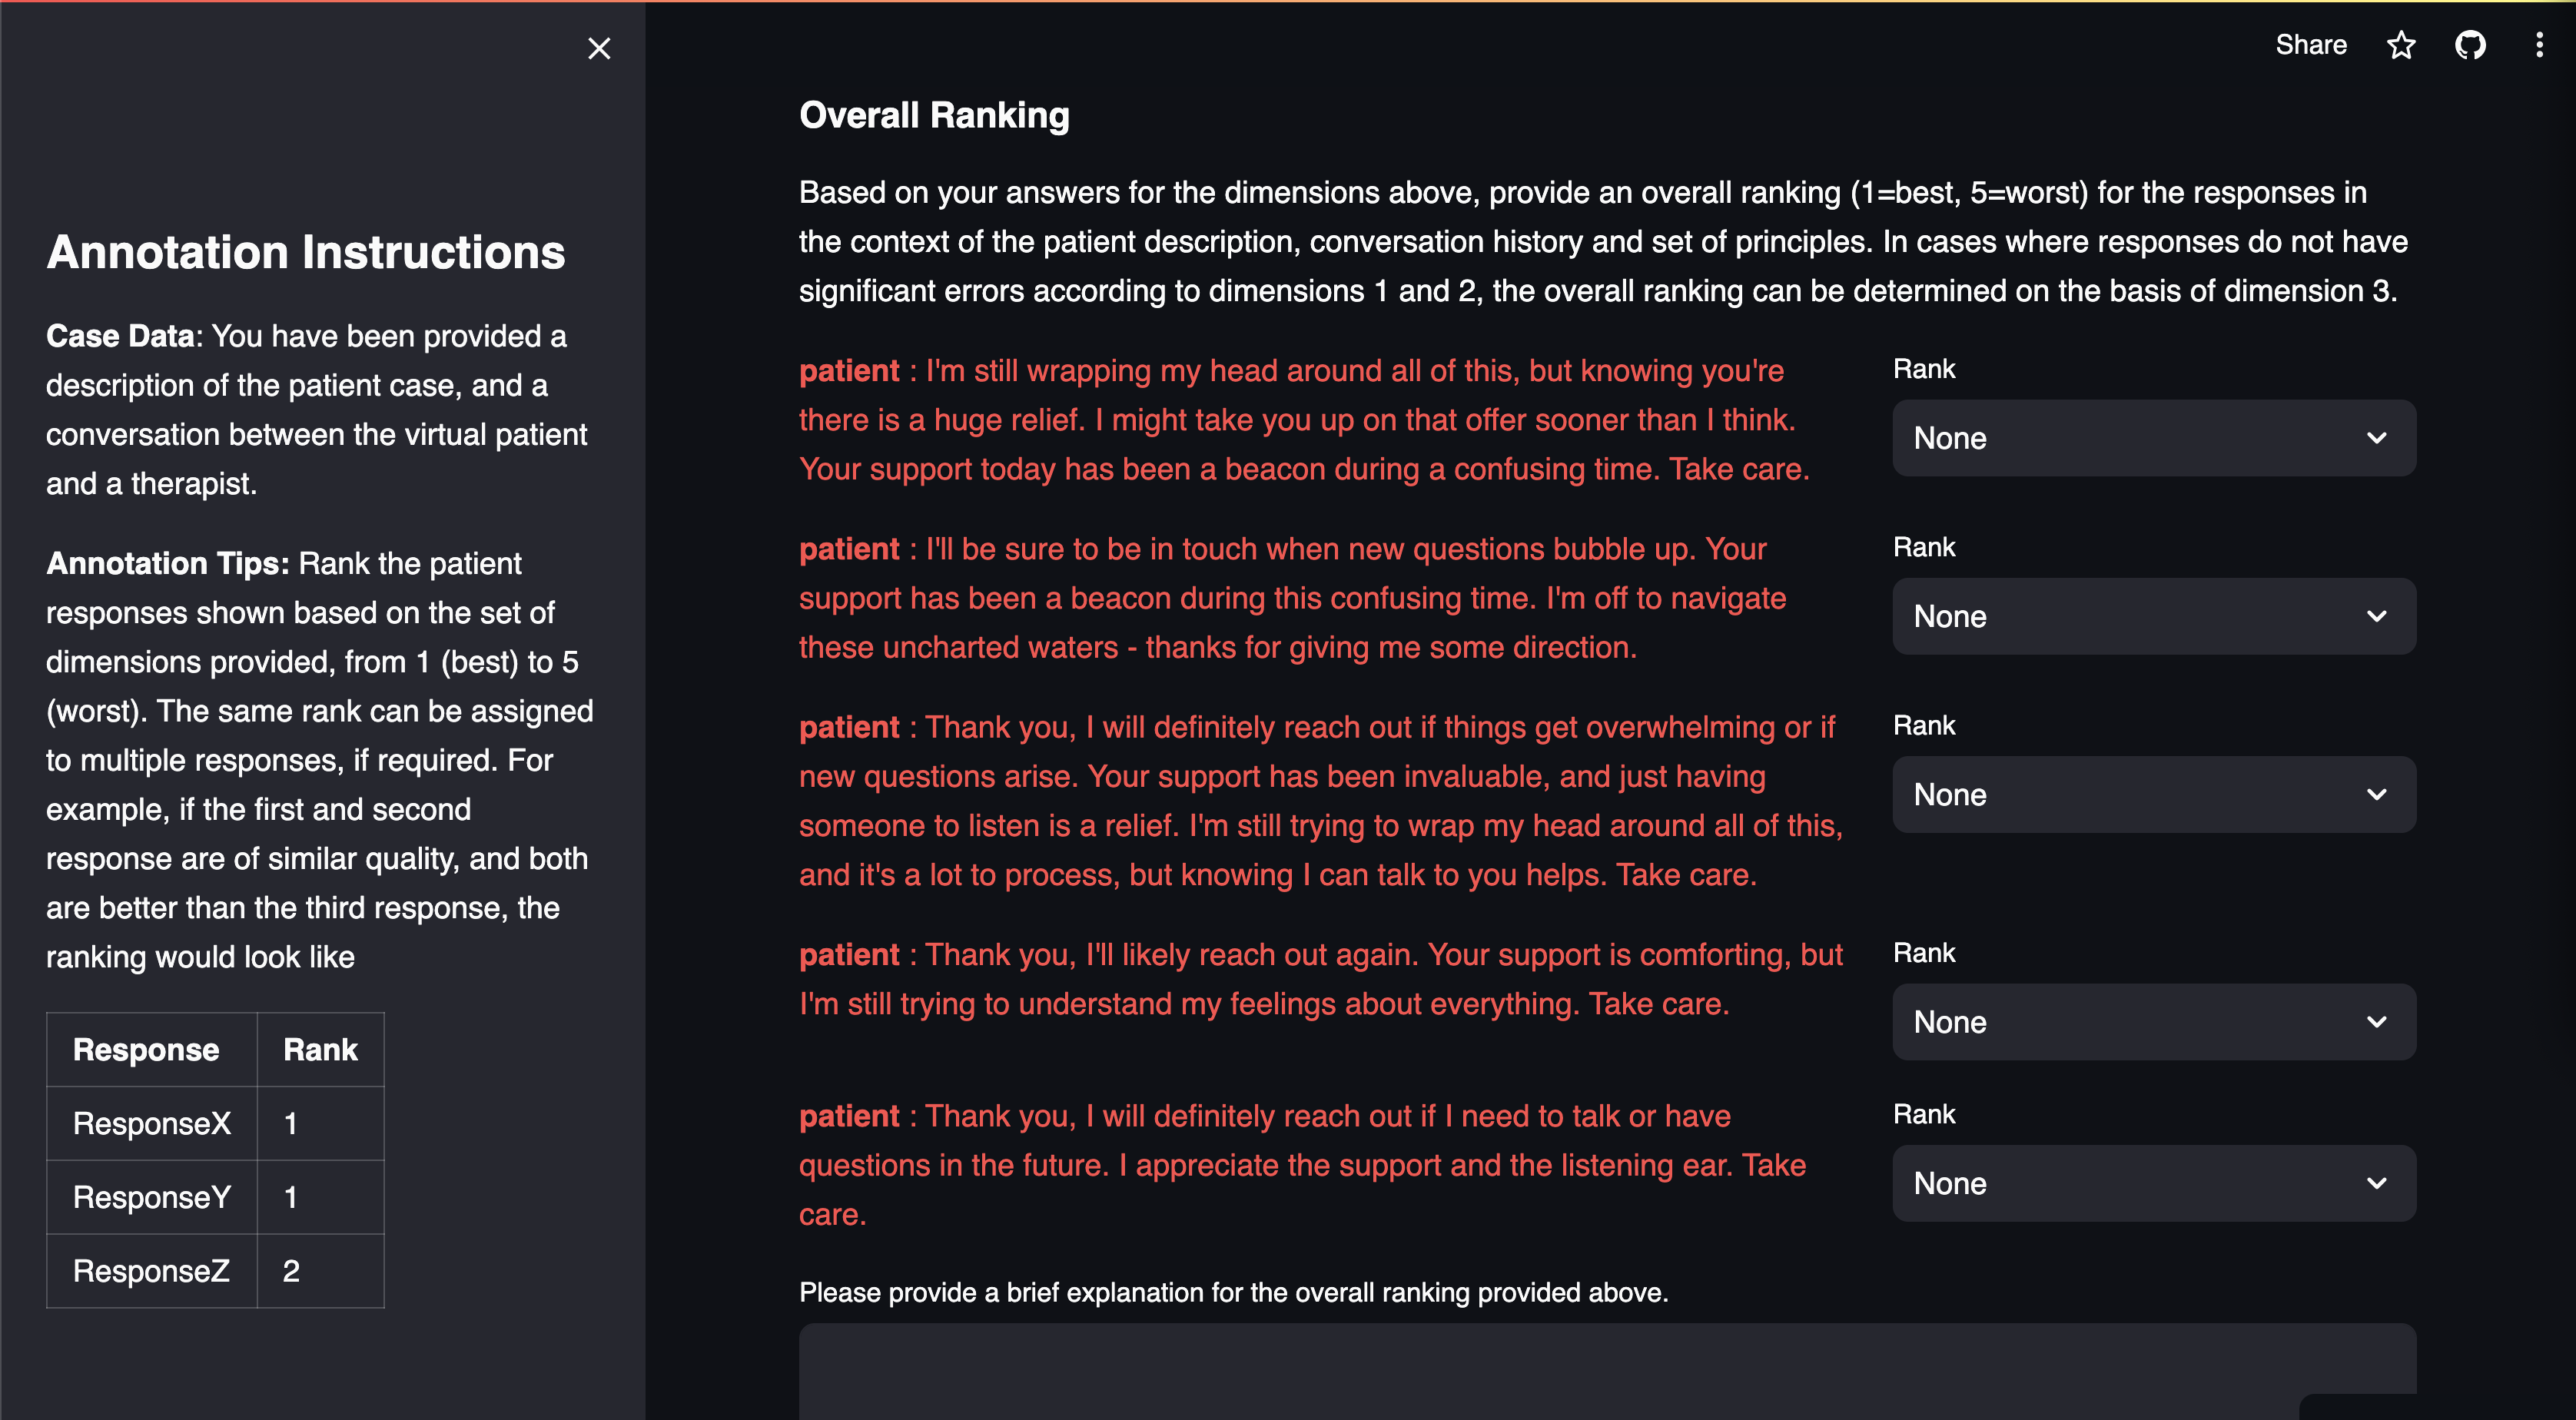
\includegraphics[width=\textwidth]{Study Screenshots/response-ranking-annotation-interface/overall.png}
    \caption{Principle Adherence Annotation Interface: Questions to get annotations for an \textbf{Overall} ranking, which also includes a free text field to capture a rationale.}
    \label{fig:ranking-interface-overall}
\end{figure*}

\end{document}
